% Options for packages loaded elsewhere
\PassOptionsToPackage{unicode}{hyperref}
\PassOptionsToPackage{hyphens}{url}
%
\documentclass[
]{article}
\usepackage{lmodern}
\usepackage{amssymb,amsmath}
\usepackage{ifxetex,ifluatex}
\ifnum 0\ifxetex 1\fi\ifluatex 1\fi=0 % if pdftex
  \usepackage[T1]{fontenc}
  \usepackage[utf8]{inputenc}
  \usepackage{textcomp} % provide euro and other symbols
\else % if luatex or xetex
  \usepackage{unicode-math}
  \defaultfontfeatures{Scale=MatchLowercase}
  \defaultfontfeatures[\rmfamily]{Ligatures=TeX,Scale=1}
\fi
% Use upquote if available, for straight quotes in verbatim environments
\IfFileExists{upquote.sty}{\usepackage{upquote}}{}
\IfFileExists{microtype.sty}{% use microtype if available
  \usepackage[]{microtype}
  \UseMicrotypeSet[protrusion]{basicmath} % disable protrusion for tt fonts
}{}
\makeatletter
\@ifundefined{KOMAClassName}{% if non-KOMA class
  \IfFileExists{parskip.sty}{%
    \usepackage{parskip}
  }{% else
    \setlength{\parindent}{0pt}
    \setlength{\parskip}{6pt plus 2pt minus 1pt}}
}{% if KOMA class
  \KOMAoptions{parskip=half}}
\makeatother
\usepackage{xcolor}
\IfFileExists{xurl.sty}{\usepackage{xurl}}{} % add URL line breaks if available
\IfFileExists{bookmark.sty}{\usepackage{bookmark}}{\usepackage{hyperref}}
\hypersetup{
  pdftitle={MOFA exploration},
  hidelinks,
  pdfcreator={LaTeX via pandoc}}
\urlstyle{same} % disable monospaced font for URLs
\usepackage[margin=1in]{geometry}
\usepackage{color}
\usepackage{fancyvrb}
\newcommand{\VerbBar}{|}
\newcommand{\VERB}{\Verb[commandchars=\\\{\}]}
\DefineVerbatimEnvironment{Highlighting}{Verbatim}{commandchars=\\\{\}}
% Add ',fontsize=\small' for more characters per line
\usepackage{framed}
\definecolor{shadecolor}{RGB}{248,248,248}
\newenvironment{Shaded}{\begin{snugshade}}{\end{snugshade}}
\newcommand{\AlertTok}[1]{\textcolor[rgb]{0.94,0.16,0.16}{#1}}
\newcommand{\AnnotationTok}[1]{\textcolor[rgb]{0.56,0.35,0.01}{\textbf{\textit{#1}}}}
\newcommand{\AttributeTok}[1]{\textcolor[rgb]{0.77,0.63,0.00}{#1}}
\newcommand{\BaseNTok}[1]{\textcolor[rgb]{0.00,0.00,0.81}{#1}}
\newcommand{\BuiltInTok}[1]{#1}
\newcommand{\CharTok}[1]{\textcolor[rgb]{0.31,0.60,0.02}{#1}}
\newcommand{\CommentTok}[1]{\textcolor[rgb]{0.56,0.35,0.01}{\textit{#1}}}
\newcommand{\CommentVarTok}[1]{\textcolor[rgb]{0.56,0.35,0.01}{\textbf{\textit{#1}}}}
\newcommand{\ConstantTok}[1]{\textcolor[rgb]{0.00,0.00,0.00}{#1}}
\newcommand{\ControlFlowTok}[1]{\textcolor[rgb]{0.13,0.29,0.53}{\textbf{#1}}}
\newcommand{\DataTypeTok}[1]{\textcolor[rgb]{0.13,0.29,0.53}{#1}}
\newcommand{\DecValTok}[1]{\textcolor[rgb]{0.00,0.00,0.81}{#1}}
\newcommand{\DocumentationTok}[1]{\textcolor[rgb]{0.56,0.35,0.01}{\textbf{\textit{#1}}}}
\newcommand{\ErrorTok}[1]{\textcolor[rgb]{0.64,0.00,0.00}{\textbf{#1}}}
\newcommand{\ExtensionTok}[1]{#1}
\newcommand{\FloatTok}[1]{\textcolor[rgb]{0.00,0.00,0.81}{#1}}
\newcommand{\FunctionTok}[1]{\textcolor[rgb]{0.00,0.00,0.00}{#1}}
\newcommand{\ImportTok}[1]{#1}
\newcommand{\InformationTok}[1]{\textcolor[rgb]{0.56,0.35,0.01}{\textbf{\textit{#1}}}}
\newcommand{\KeywordTok}[1]{\textcolor[rgb]{0.13,0.29,0.53}{\textbf{#1}}}
\newcommand{\NormalTok}[1]{#1}
\newcommand{\OperatorTok}[1]{\textcolor[rgb]{0.81,0.36,0.00}{\textbf{#1}}}
\newcommand{\OtherTok}[1]{\textcolor[rgb]{0.56,0.35,0.01}{#1}}
\newcommand{\PreprocessorTok}[1]{\textcolor[rgb]{0.56,0.35,0.01}{\textit{#1}}}
\newcommand{\RegionMarkerTok}[1]{#1}
\newcommand{\SpecialCharTok}[1]{\textcolor[rgb]{0.00,0.00,0.00}{#1}}
\newcommand{\SpecialStringTok}[1]{\textcolor[rgb]{0.31,0.60,0.02}{#1}}
\newcommand{\StringTok}[1]{\textcolor[rgb]{0.31,0.60,0.02}{#1}}
\newcommand{\VariableTok}[1]{\textcolor[rgb]{0.00,0.00,0.00}{#1}}
\newcommand{\VerbatimStringTok}[1]{\textcolor[rgb]{0.31,0.60,0.02}{#1}}
\newcommand{\WarningTok}[1]{\textcolor[rgb]{0.56,0.35,0.01}{\textbf{\textit{#1}}}}
\usepackage{graphicx,grffile}
\makeatletter
\def\maxwidth{\ifdim\Gin@nat@width>\linewidth\linewidth\else\Gin@nat@width\fi}
\def\maxheight{\ifdim\Gin@nat@height>\textheight\textheight\else\Gin@nat@height\fi}
\makeatother
% Scale images if necessary, so that they will not overflow the page
% margins by default, and it is still possible to overwrite the defaults
% using explicit options in \includegraphics[width, height, ...]{}
\setkeys{Gin}{width=\maxwidth,height=\maxheight,keepaspectratio}
% Set default figure placement to htbp
\makeatletter
\def\fps@figure{htbp}
\makeatother
\setlength{\emergencystretch}{3em} % prevent overfull lines
\providecommand{\tightlist}{%
  \setlength{\itemsep}{0pt}\setlength{\parskip}{0pt}}
\setcounter{secnumdepth}{-\maxdimen} % remove section numbering

\title{MOFA exploration}
\author{}
\date{\vspace{-2.5em}}

\begin{document}
\maketitle

\begin{Shaded}
\begin{Highlighting}[]
\KeywordTok{library}\NormalTok{(tidyverse)}
\end{Highlighting}
\end{Shaded}

\begin{verbatim}
## Warning: package 'tidyverse' was built under R version 4.0.3
\end{verbatim}

\begin{verbatim}
## -- Attaching packages --------------------------------------- tidyverse 1.3.0 --
\end{verbatim}

\begin{verbatim}
## v ggplot2 3.3.1     v purrr   0.3.4
## v tibble  3.0.1     v dplyr   1.0.0
## v tidyr   1.1.0     v stringr 1.4.0
## v readr   1.3.1     v forcats 0.5.0
\end{verbatim}

\begin{verbatim}
## Warning: package 'purrr' was built under R version 4.0.3
\end{verbatim}

\begin{verbatim}
## Warning: package 'stringr' was built under R version 4.0.3
\end{verbatim}

\begin{verbatim}
## -- Conflicts ------------------------------------------ tidyverse_conflicts() --
## x dplyr::filter() masks stats::filter()
## x dplyr::lag()    masks stats::lag()
\end{verbatim}

\begin{Shaded}
\begin{Highlighting}[]
\KeywordTok{library}\NormalTok{(MOFA2)}
\end{Highlighting}
\end{Shaded}

\begin{verbatim}
## 
## Attaching package: 'MOFA2'
\end{verbatim}

\begin{verbatim}
## The following object is masked from 'package:stats':
## 
##     predict
\end{verbatim}

\begin{Shaded}
\begin{Highlighting}[]
\KeywordTok{library}\NormalTok{(here)}
\end{Highlighting}
\end{Shaded}

\begin{verbatim}
## here() starts at /home/rstudio/promise
\end{verbatim}

\begin{Shaded}
\begin{Highlighting}[]
\CommentTok{#library(MOFAdata)}
\KeywordTok{library}\NormalTok{(ReactomePA)}
\end{Highlighting}
\end{Shaded}

\begin{verbatim}
## 
\end{verbatim}

\begin{verbatim}
## ReactomePA v1.34.0  For help: https://guangchuangyu.github.io/ReactomePA
## 
## If you use ReactomePA in published research, please cite:
## Guangchuang Yu, Qing-Yu He. ReactomePA: an R/Bioconductor package for reactome pathway analysis and visualization. Molecular BioSystems 2016, 12(2):477-479
\end{verbatim}

\begin{Shaded}
\begin{Highlighting}[]
\KeywordTok{library}\NormalTok{(biomaRt)}
\KeywordTok{library}\NormalTok{(cowplot)}
\end{Highlighting}
\end{Shaded}

\begin{verbatim}
## 
## ********************************************************
\end{verbatim}

\begin{verbatim}
## Note: As of version 1.0.0, cowplot does not change the
\end{verbatim}

\begin{verbatim}
##   default ggplot2 theme anymore. To recover the previous
\end{verbatim}

\begin{verbatim}
##   behavior, execute:
##   theme_set(theme_cowplot())
\end{verbatim}

\begin{verbatim}
## ********************************************************
\end{verbatim}

\begin{Shaded}
\begin{Highlighting}[]
\KeywordTok{library}\NormalTok{(enrichplot)}
\KeywordTok{library}\NormalTok{(dplyr)}
\KeywordTok{library}\NormalTok{(clusterProfiler)}
\end{Highlighting}
\end{Shaded}

\begin{verbatim}
## clusterProfiler v3.18.1  For help: https://guangchuangyu.github.io/software/clusterProfiler
## 
## If you use clusterProfiler in published research, please cite:
## Guangchuang Yu, Li-Gen Wang, Yanyan Han, Qing-Yu He. clusterProfiler: an R package for comparing biological themes among gene clusters. OMICS: A Journal of Integrative Biology. 2012, 16(5):284-287.
\end{verbatim}

\begin{verbatim}
## 
## Attaching package: 'clusterProfiler'
\end{verbatim}

\begin{verbatim}
## The following object is masked from 'package:biomaRt':
## 
##     select
\end{verbatim}

\begin{verbatim}
## The following object is masked from 'package:purrr':
## 
##     simplify
\end{verbatim}

\begin{verbatim}
## The following object is masked from 'package:stats':
## 
##     filter
\end{verbatim}

\begin{Shaded}
\begin{Highlighting}[]
\KeywordTok{library}\NormalTok{(utils)}
\KeywordTok{library}\NormalTok{(stats)}
\end{Highlighting}
\end{Shaded}

\begin{Shaded}
\begin{Highlighting}[]
\CommentTok{# input}
\NormalTok{model <-}\StringTok{ }\KeywordTok{load_model}\NormalTok{(}\KeywordTok{here}\NormalTok{(}\StringTok{"models/mofa/model.hdf5"}\NormalTok{))}

\CommentTok{# gene expression data}
\NormalTok{promise_long_filtered_top <-}\StringTok{ }\KeywordTok{readRDS}\NormalTok{(here}\OperatorTok{::}\KeywordTok{here}\NormalTok{(}\StringTok{'data/processed/expression/promise_expr_filtered_tidy_top.rds'}\NormalTok{))}

\CommentTok{# organoid morphology}
\NormalTok{umap_df <-}\StringTok{ }\KeywordTok{readRDS}\NormalTok{(here}\OperatorTok{::}\KeywordTok{here}\NormalTok{(}\StringTok{"data/processed/PhenotypeSpectrum/umap_absolute_all_drugs_sampled.Rds"}\NormalTok{))}

\CommentTok{# organoid size}
\NormalTok{organoid_size_fit <-}\StringTok{ }\KeywordTok{readRDS}\NormalTok{(here}\OperatorTok{::}\KeywordTok{here}\NormalTok{(}\StringTok{"data/processed/morphology/organoid_size.Rds"}\NormalTok{)) }\OperatorTok\StringTok{ }
\StringTok{  }\KeywordTok{filter}\NormalTok{(}\OperatorTok{!}\NormalTok{line }\OperatorTok\StringTok{ }\KeywordTok{c}\NormalTok{(}\StringTok{'D055T01'}\NormalTok{, }\StringTok{'D020T02'}\NormalTok{, }\StringTok{'D021T01'}\NormalTok{)) }\OperatorTok\StringTok{ }
\StringTok{  }\CommentTok{#filter(!line %in% c('D055T01','D020T02')) %>% }
\StringTok{  }\KeywordTok{mutate}\NormalTok{(}\DataTypeTok{line =} \KeywordTok{as.character}\NormalTok{(line)) }\OperatorTok\StringTok{ }
\StringTok{  }\NormalTok{dplyr}\OperatorTok{::}\KeywordTok{select}\NormalTok{(line, }\DataTypeTok{size =}\NormalTok{ x, }\DataTypeTok{rep =}\NormalTok{ replicate) }\OperatorTok\StringTok{ }
\StringTok{  }\KeywordTok{distinct}\NormalTok{() }\OperatorTok\StringTok{ }\KeywordTok{arrange}\NormalTok{(line) }\OperatorTok
\StringTok{  }\KeywordTok{mutate}\NormalTok{(}\DataTypeTok{line =} \KeywordTok{substr}\NormalTok{(line, }\DecValTok{1}\NormalTok{, }\DecValTok{4}\NormalTok{)) }\OperatorTok\StringTok{ }
\StringTok{  }\KeywordTok{mutate}\NormalTok{(}\DataTypeTok{rep =} \KeywordTok{paste0}\NormalTok{(}\StringTok{"r"}\NormalTok{, rep))}

\CommentTok{# morphology classification}
\NormalTok{organoid_morphology <-}\StringTok{ }\KeywordTok{read_delim}\NormalTok{(here}\OperatorTok{::}\KeywordTok{here}\NormalTok{(}\StringTok{"references/imaging/visual_classification_organoids.csv"}\NormalTok{), }\StringTok{";"}\NormalTok{, }\DataTypeTok{escape_double =} \OtherTok{FALSE}\NormalTok{, }\DataTypeTok{trim_ws =} \OtherTok{TRUE}\NormalTok{) }\OperatorTok\StringTok{ }
\StringTok{  }\NormalTok{dplyr}\OperatorTok{::}\KeywordTok{select}\NormalTok{(}\DataTypeTok{line =}\NormalTok{ organoid, }\DataTypeTok{morphology =}\NormalTok{ visual_inspection_v2) }\OperatorTok
\StringTok{  }\KeywordTok{mutate}\NormalTok{(}\DataTypeTok{line =} \KeywordTok{substr}\NormalTok{(line, }\DecValTok{1}\NormalTok{, }\DecValTok{4}\NormalTok{)) }\OperatorTok\StringTok{ }
\StringTok{  }\KeywordTok{mutate}\NormalTok{(}\DataTypeTok{morphology =} \KeywordTok{if_else}\NormalTok{(}\KeywordTok{is.na}\NormalTok{(morphology), }\StringTok{"other"}\NormalTok{, morphology))}
\end{Highlighting}
\end{Shaded}

\begin{verbatim}
## Parsed with column specification:
## cols(
##   organoid = col_character(),
##   visual_inspection_morphology_2017 = col_character(),
##   visual_class_2_2017 = col_double(),
##   visual_inspection_v2 = col_character(),
##   visual_inspection_size_2017 = col_character(),
##   visual_class_1_2017 = col_double(),
##   visual_size_ranking_2018 = col_double(),
##   visual_cystic_ranking_2018 = col_double(),
##   clustering_jan = col_character()
## )
\end{verbatim}

\begin{Shaded}
\begin{Highlighting}[]
\CommentTok{# drug activity data}
\NormalTok{utils}\OperatorTok{::}\KeywordTok{data}\NormalTok{(}\StringTok{'aucroc'}\NormalTok{, }\DataTypeTok{package =} \StringTok{'SCOPEAnalysis'}\NormalTok{)}
\NormalTok{drug_activity <-}\StringTok{ }\NormalTok{aucroc }\OperatorTok\StringTok{ }\KeywordTok{filter}\NormalTok{(}\OperatorTok{!}\NormalTok{line }\OperatorTok\StringTok{ }\KeywordTok{c}\NormalTok{(}\StringTok{'D055T01'}\NormalTok{, }\StringTok{'D021T01'}\NormalTok{, }\StringTok{'D054T01'}\NormalTok{))}

\CommentTok{# gene expression annotation }
\NormalTok{intestinal_sig <-}\StringTok{ }\NormalTok{readxl}\OperatorTok{::}\KeywordTok{read_excel}\NormalTok{(}\KeywordTok{here}\NormalTok{(}\StringTok{'data/external/expression/merloz-suarez_sigantures.xls'}\NormalTok{), }
                                     \DataTypeTok{sheet =} \DecValTok{1}\NormalTok{, }\DataTypeTok{skip =} \DecValTok{4}\NormalTok{) }\OperatorTok\StringTok{ }\NormalTok{.[,}\DecValTok{1}\OperatorTok{:}\DecValTok{4}\NormalTok{] }\OperatorTok
\StringTok{  }\KeywordTok{gather}\NormalTok{(signature, symbol) }\OperatorTok\StringTok{ }\KeywordTok{drop_na}\NormalTok{() }\OperatorTok\StringTok{ }
\StringTok{  }\KeywordTok{mutate}\NormalTok{(}\DataTypeTok{symbol =} \KeywordTok{gsub}\NormalTok{(}\StringTok{'}\CharTok{\textbackslash{}\textbackslash{}}\StringTok{*'}\NormalTok{, }\StringTok{''}\NormalTok{, symbol))}
\end{Highlighting}
\end{Shaded}

\begin{verbatim}
## New names:
## * `` -> ...5
\end{verbatim}

\begin{Shaded}
\begin{Highlighting}[]
\NormalTok{cris_sig <-}\StringTok{ }\NormalTok{readxl}\OperatorTok{::}\KeywordTok{read_excel}\NormalTok{(}\KeywordTok{here}\NormalTok{(}\StringTok{'data/external/expression/cris/41467_2017_BFncomms15107_MOESM422_ESM.xlsx'}\NormalTok{), }\DataTypeTok{sheet =} \DecValTok{1}\NormalTok{, }\DataTypeTok{skip =} \DecValTok{2}\NormalTok{) }\OperatorTok\StringTok{ }
\StringTok{  }\NormalTok{dplyr}\OperatorTok{::}\KeywordTok{rename}\NormalTok{(}\DataTypeTok{symbol =} \StringTok{`}\DataTypeTok{Gene ID}\StringTok{`}\NormalTok{, }\DataTypeTok{signature =} \StringTok{`}\DataTypeTok{CRIS Class}\StringTok{`}\NormalTok{)}

\CommentTok{# organoid mutation}
\NormalTok{mofa_genetics <-}\StringTok{ }\KeywordTok{read_delim}\NormalTok{(here}\OperatorTok{::}\KeywordTok{here}\NormalTok{(}\StringTok{"data/processed/mutation/Table-S2_Mutations_PDOs_RevisionV4.csv"}\NormalTok{), }\DataTypeTok{delim =} \StringTok{";"}\NormalTok{) }\OperatorTok\StringTok{ }
\StringTok{    }\NormalTok{janitor}\OperatorTok{::}\KeywordTok{clean_names}\NormalTok{() }\OperatorTok\StringTok{ }
\StringTok{    }\KeywordTok{mutate}\NormalTok{(}\DataTypeTok{sample =} \KeywordTok{substr}\NormalTok{(sample, }\DecValTok{2}\NormalTok{,}\KeywordTok{nchar}\NormalTok{(sample)}\OperatorTok{-}\DecValTok{1}\NormalTok{)) }\OperatorTok\StringTok{ }
\StringTok{    }\KeywordTok{mutate}\NormalTok{(}\DataTypeTok{sample =} \KeywordTok{paste0}\NormalTok{(}\StringTok{"D"}\NormalTok{, sample)) }\OperatorTok\StringTok{ }
\StringTok{    }\NormalTok{dplyr}\OperatorTok{::}\KeywordTok{filter}\NormalTok{(}\OperatorTok{!}\NormalTok{sample }\OperatorTok\StringTok{ }\KeywordTok{c}\NormalTok{(}\StringTok{"D021"}\NormalTok{, }\StringTok{"D015"}\NormalTok{)) }\OperatorTok
\StringTok{    }\KeywordTok{expand_grid}\NormalTok{(}\DataTypeTok{replicate =} \KeywordTok{c}\NormalTok{(}\StringTok{"r1"}\NormalTok{, }\StringTok{"r2"}\NormalTok{)) }\OperatorTok\StringTok{ }
\StringTok{    }\KeywordTok{mutate}\NormalTok{(}\DataTypeTok{sample =} \KeywordTok{paste0}\NormalTok{(sample, }\StringTok{"_"}\NormalTok{, replicate)) }\OperatorTok\StringTok{ }
\StringTok{    }\NormalTok{dplyr}\OperatorTok{::}\KeywordTok{select}\NormalTok{(sample, }\DataTypeTok{feature =}\NormalTok{ symbol, }\KeywordTok{everything}\NormalTok{()) }\OperatorTok\StringTok{ }\NormalTok{dplyr}\OperatorTok{::}\KeywordTok{select}\NormalTok{(sample, feature) }\OperatorTok\StringTok{ }
\StringTok{    }\KeywordTok{mutate}\NormalTok{(}\DataTypeTok{value =} \DecValTok{1}\NormalTok{) }\OperatorTok
\StringTok{    }\KeywordTok{complete}\NormalTok{(sample, feature, }\DataTypeTok{fill =} \KeywordTok{list}\NormalTok{(}\DataTypeTok{value =} \DecValTok{0}\NormalTok{)) }\OperatorTok\StringTok{ }
\StringTok{    }\KeywordTok{distinct}\NormalTok{(sample, feature, value) }\OperatorTok
\StringTok{    }\KeywordTok{mutate}\NormalTok{(}\DataTypeTok{view =} \StringTok{"mutation"}\NormalTok{)}
\end{Highlighting}
\end{Shaded}

\begin{verbatim}
## Parsed with column specification:
## cols(
##   SAMPLE = col_character(),
##   SYMBOL = col_character(),
##   Protein_position = col_character(),
##   Amino_acids = col_character(),
##   Consequence = col_character()
## )
\end{verbatim}

\begin{Shaded}
\begin{Highlighting}[]
\NormalTok{weights <-}\StringTok{ }\NormalTok{model}\OperatorTok{@}\NormalTok{expectations}\OperatorTok{$}\NormalTok{Z}\OperatorTok{$}\NormalTok{single_group }\OperatorTok\StringTok{ }\KeywordTok{as.data.frame}\NormalTok{() }\OperatorTok\StringTok{ }\KeywordTok{rownames_to_column}\NormalTok{(}\StringTok{"id"}\NormalTok{) }\OperatorTok\StringTok{ }\KeywordTok{as_tibble}\NormalTok{() }\OperatorTok\StringTok{ }\NormalTok{janitor}\OperatorTok{::}\KeywordTok{clean_names}\NormalTok{()}
\NormalTok{loadings_size <-}\StringTok{ }\NormalTok{model}\OperatorTok{@}\NormalTok{expectations}\OperatorTok{$}\NormalTok{W}\OperatorTok{$}\NormalTok{size_view }\OperatorTok\StringTok{ }\KeywordTok{as.data.frame}\NormalTok{() }\OperatorTok\StringTok{ }\KeywordTok{rownames_to_column}\NormalTok{(}\StringTok{"id"}\NormalTok{) }\OperatorTok\StringTok{ }\KeywordTok{as_tibble}\NormalTok{() }\OperatorTok\StringTok{ }\NormalTok{janitor}\OperatorTok{::}\KeywordTok{clean_names}\NormalTok{()}
\NormalTok{loadings_expression <-}\StringTok{ }\NormalTok{model}\OperatorTok{@}\NormalTok{expectations}\OperatorTok{$}\NormalTok{W}\OperatorTok{$}\NormalTok{expression }\OperatorTok\StringTok{ }\KeywordTok{as.data.frame}\NormalTok{() }\OperatorTok\StringTok{ }\KeywordTok{rownames_to_column}\NormalTok{(}\StringTok{"id"}\NormalTok{) }\OperatorTok\StringTok{ }\KeywordTok{as_tibble}\NormalTok{() }\OperatorTok\StringTok{ }\NormalTok{janitor}\OperatorTok{::}\KeywordTok{clean_names}\NormalTok{()}
\NormalTok{loadings_morphology <-}\StringTok{ }\NormalTok{model}\OperatorTok{@}\NormalTok{expectations}\OperatorTok{$}\NormalTok{W}\OperatorTok{$}\NormalTok{morphology }\OperatorTok\StringTok{ }\KeywordTok{as.data.frame}\NormalTok{() }\OperatorTok\StringTok{ }\KeywordTok{rownames_to_column}\NormalTok{(}\StringTok{"id"}\NormalTok{) }\OperatorTok\StringTok{ }\KeywordTok{as_tibble}\NormalTok{() }\OperatorTok\StringTok{ }\NormalTok{janitor}\OperatorTok{::}\KeywordTok{clean_names}\NormalTok{()}
\NormalTok{loadings_drug_activity <-}\StringTok{ }\NormalTok{model}\OperatorTok{@}\NormalTok{expectations}\OperatorTok{$}\NormalTok{W}\OperatorTok{$}\NormalTok{drug_activity }\OperatorTok\StringTok{ }\KeywordTok{as.data.frame}\NormalTok{() }\OperatorTok\StringTok{ }\KeywordTok{rownames_to_column}\NormalTok{(}\StringTok{"id"}\NormalTok{) }\OperatorTok\StringTok{ }\KeywordTok{as_tibble}\NormalTok{() }\OperatorTok\StringTok{ }\NormalTok{janitor}\OperatorTok{::}\KeywordTok{clean_names}\NormalTok{()}
\NormalTok{loadings_mutation <-}\StringTok{ }\NormalTok{model}\OperatorTok{@}\NormalTok{expectations}\OperatorTok{$}\NormalTok{W}\OperatorTok{$}\NormalTok{mutation }\OperatorTok\StringTok{ }\KeywordTok{as.data.frame}\NormalTok{() }\OperatorTok\StringTok{ }\KeywordTok{rownames_to_column}\NormalTok{(}\StringTok{"id"}\NormalTok{) }\OperatorTok\StringTok{ }\KeywordTok{as_tibble}\NormalTok{() }\OperatorTok\StringTok{ }\NormalTok{janitor}\OperatorTok{::}\KeywordTok{clean_names}\NormalTok{()}
\end{Highlighting}
\end{Shaded}

\hypertarget{qc}{%
\section{QC}\label{qc}}

\begin{Shaded}
\begin{Highlighting}[]
\KeywordTok{plot_data_overview}\NormalTok{(model) }\OperatorTok{+}\StringTok{ }
\StringTok{  }\KeywordTok{ggsave}\NormalTok{(here}\OperatorTok{::}\KeywordTok{here}\NormalTok{(}\StringTok{"reports/figures/mofa/data_overview.pdf"}\NormalTok{))}
\end{Highlighting}
\end{Shaded}

\begin{verbatim}
## Saving 6.5 x 4.5 in image
\end{verbatim}

\includegraphics{mofa_exploration_files/figure-latex/unnamed-chunk-3-1.pdf}

\begin{Shaded}
\begin{Highlighting}[]
\NormalTok{df <-}\StringTok{ }\KeywordTok{head}\NormalTok{(model}\OperatorTok{@}\NormalTok{cache}\OperatorTok{$}\NormalTok{variance_explained}\OperatorTok{$}\NormalTok{r2_total[[}\DecValTok{1}\NormalTok{]]) }\OperatorTok
\StringTok{  }\KeywordTok{as.data.frame}\NormalTok{() }\OperatorTok
\StringTok{  }\KeywordTok{rownames_to_column}\NormalTok{(}\StringTok{"feature"}\NormalTok{) }\OperatorTok
\StringTok{  }\NormalTok{magrittr}\OperatorTok{::}\KeywordTok{set_colnames}\NormalTok{(}\KeywordTok{c}\NormalTok{(}\StringTok{"feature"}\NormalTok{, }\StringTok{"var"}\NormalTok{)) }\OperatorTok
\StringTok{  }\KeywordTok{mutate}\NormalTok{(}\DataTypeTok{var =}\NormalTok{ var}\OperatorTok{/}\DecValTok{100}\NormalTok{)}

\NormalTok{gg_ve_feature <-}\StringTok{ }\NormalTok{df }\OperatorTok
\StringTok{  }\KeywordTok{ggplot}\NormalTok{(}\KeywordTok{aes}\NormalTok{(feature, var)) }\OperatorTok{+}\StringTok{ }
\StringTok{  }\KeywordTok{geom_bar}\NormalTok{(}\DataTypeTok{stat =} \StringTok{"identity"}\NormalTok{) }\OperatorTok{+}\StringTok{ }
\StringTok{  }\KeywordTok{coord_flip}\NormalTok{() }\OperatorTok{+}\StringTok{ }
\StringTok{  }\KeywordTok{theme_cowplot}\NormalTok{() }\OperatorTok{+}\StringTok{ }
\StringTok{  }\KeywordTok{labs}\NormalTok{(}\DataTypeTok{y =} \StringTok{"R2"}\NormalTok{)}

\NormalTok{gg_ve_feature }\OperatorTok{+}\StringTok{ }
\StringTok{  }\KeywordTok{ggsave}\NormalTok{(here}\OperatorTok{::}\KeywordTok{here}\NormalTok{(}\StringTok{"reports/figures/mofa/var_explained_feature.pdf"}\NormalTok{))}
\end{Highlighting}
\end{Shaded}

\begin{verbatim}
## Saving 6.5 x 4.5 in image
\end{verbatim}

\includegraphics{mofa_exploration_files/figure-latex/unnamed-chunk-4-1.pdf}

Breakdown by factors

\begin{Shaded}
\begin{Highlighting}[]
\NormalTok{model}\OperatorTok{@}\NormalTok{cache}\OperatorTok{$}\NormalTok{variance_explained}\OperatorTok{$}\NormalTok{r2_per_factor}\OperatorTok{$}\NormalTok{single_group}
\end{Highlighting}
\end{Shaded}

\begin{verbatim}
##         drug_activity expression morphology_view  mutation    size_view
## Factor1      16.34025   14.65149        1.294912 13.992686 3.928743e+01
## Factor2      12.26939   13.05253       15.517353  8.569222 6.883715e-02
## Factor3      12.81709   10.37798        7.372122  3.408771 3.153277e-05
\end{verbatim}

\begin{Shaded}
\begin{Highlighting}[]
\NormalTok{model}\OperatorTok{@}\NormalTok{cache}\OperatorTok{$}\NormalTok{variance_explained}\OperatorTok{$}\NormalTok{r2_per_factor}\OperatorTok{$}\NormalTok{single_group }\OperatorTok\StringTok{ }\KeywordTok{as.data.frame}\NormalTok{() }\OperatorTok\StringTok{ }
\StringTok{  }\KeywordTok{rownames_to_column}\NormalTok{(}\StringTok{"factor"}\NormalTok{) }\OperatorTok\StringTok{ }
\StringTok{  }\KeywordTok{mutate}\NormalTok{(}\DataTypeTok{overall_variance =}\NormalTok{ expression }\OperatorTok{+}\StringTok{ }\NormalTok{morphology_view }\OperatorTok{+}\StringTok{ }\NormalTok{size_view }\OperatorTok{+}\StringTok{ }\NormalTok{drug_activity) }\OperatorTok
\StringTok{  }\KeywordTok{mutate}\NormalTok{(}\DataTypeTok{overall_variance =}\NormalTok{ overall_variance}\OperatorTok{/}\DecValTok{4}\NormalTok{) }\OperatorTok
\StringTok{  }\KeywordTok{ggplot}\NormalTok{(}\KeywordTok{aes}\NormalTok{(factor, overall_variance)) }\OperatorTok{+}\StringTok{ }
\StringTok{  }\KeywordTok{geom_point}\NormalTok{(}\DataTypeTok{size =} \DecValTok{2}\NormalTok{) }\OperatorTok{+}\StringTok{ }
\StringTok{  }\KeywordTok{theme_cowplot}\NormalTok{()}
\end{Highlighting}
\end{Shaded}

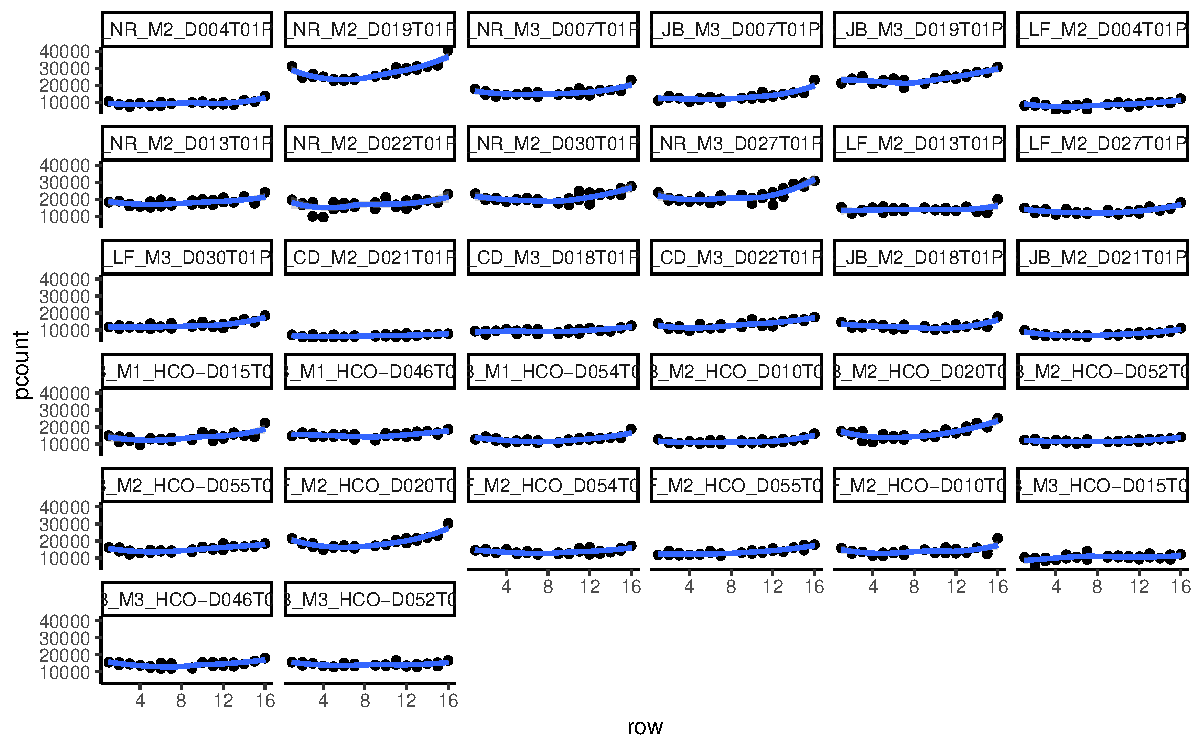
\includegraphics{mofa_exploration_files/figure-latex/unnamed-chunk-6-1.pdf}

\begin{Shaded}
\begin{Highlighting}[]
\NormalTok{gg_ve <-}\StringTok{ }\KeywordTok{plot_variance_explained}\NormalTok{(model, }\DataTypeTok{x=}\StringTok{"view"}\NormalTok{, }\DataTypeTok{y=}\StringTok{"factor"}\NormalTok{) }\OperatorTok{+}\StringTok{ }\KeywordTok{coord_flip}\NormalTok{() }\OperatorTok{+}
\StringTok{  }\KeywordTok{theme_cowplot}\NormalTok{() }
\NormalTok{gg_ve  }\OperatorTok{+}\StringTok{ }
\StringTok{  }\CommentTok{#coord_equal() +}
\StringTok{  }\KeywordTok{ggsave}\NormalTok{(here}\OperatorTok{::}\KeywordTok{here}\NormalTok{(}\StringTok{"reports/figures/mofa/var_explained.pdf"}\NormalTok{))}
\end{Highlighting}
\end{Shaded}

\begin{verbatim}
## Saving 6.5 x 4.5 in image
\end{verbatim}

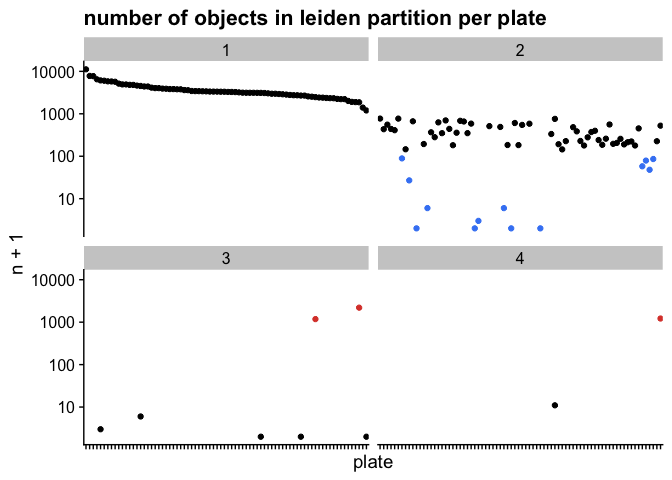
\includegraphics{mofa_exploration_files/figure-latex/unnamed-chunk-7-1.pdf}

\begin{Shaded}
\begin{Highlighting}[]
\NormalTok{ph_cor <-}\StringTok{ }\NormalTok{weights }\OperatorTok\StringTok{ }
\StringTok{  }\KeywordTok{as.data.frame}\NormalTok{() }\OperatorTok\StringTok{ }
\StringTok{  }\KeywordTok{column_to_rownames}\NormalTok{(}\StringTok{"id"}\NormalTok{) }\OperatorTok\StringTok{ }
\StringTok{  }\KeywordTok{cor}\NormalTok{() }\OperatorTok\StringTok{ }
\StringTok{  }\NormalTok{pheatmap}\OperatorTok{::}\KeywordTok{pheatmap}\NormalTok{()}
\end{Highlighting}
\end{Shaded}

\includegraphics{mofa_exploration_files/figure-latex/unnamed-chunk-8-1.pdf}

\begin{Shaded}
\begin{Highlighting}[]
\NormalTok{weights }\OperatorTok\StringTok{ }
\StringTok{  }\KeywordTok{as.data.frame}\NormalTok{() }\OperatorTok\StringTok{ }
\StringTok{  }\KeywordTok{column_to_rownames}\NormalTok{(}\StringTok{"id"}\NormalTok{) }\OperatorTok\StringTok{ }
\StringTok{  }\KeywordTok{cor}\NormalTok{() }\OperatorTok\StringTok{ }\KeywordTok{as.vector}\NormalTok{() }\OperatorTok\StringTok{ }
\StringTok{  }\NormalTok{.[. }\OperatorTok{!=}\StringTok{ }\DecValTok{1}\NormalTok{] }\OperatorTok\StringTok{ }
\StringTok{  }\KeywordTok{summary}\NormalTok{()}
\end{Highlighting}
\end{Shaded}

\begin{verbatim}
##      Min.   1st Qu.    Median      Mean   3rd Qu.      Max. 
## -0.115158 -0.085003  0.005465 -0.029503  0.017255  0.021185
\end{verbatim}

\begin{Shaded}
\begin{Highlighting}[]
\KeywordTok{plot_factor}\NormalTok{(model, }
  \DataTypeTok{factor =} \DecValTok{1}\OperatorTok{:}\DecValTok{3}
\NormalTok{)}
\end{Highlighting}
\end{Shaded}

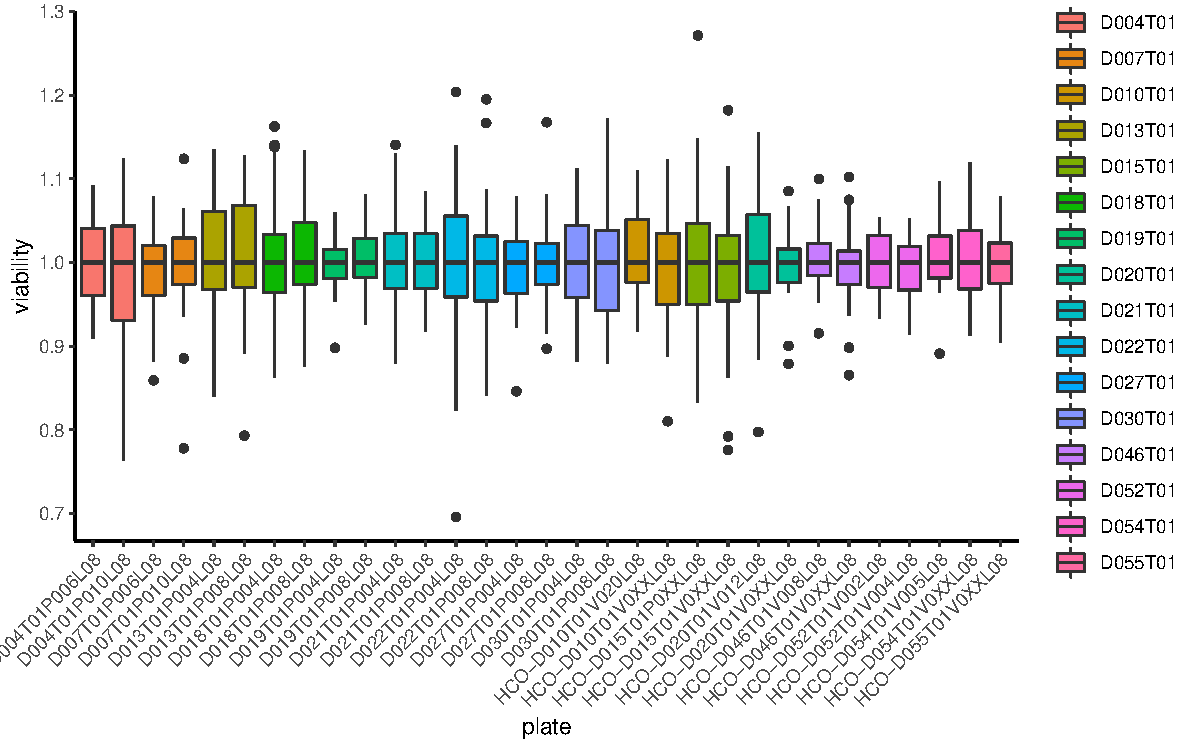
\includegraphics{mofa_exploration_files/figure-latex/unnamed-chunk-10-1.pdf}

\hypertarget{factor-overview}{%
\section{factor overview}\label{factor-overview}}

\begin{Shaded}
\begin{Highlighting}[]
\NormalTok{umap_factor <-}\StringTok{ }\NormalTok{weights }\OperatorTok\StringTok{ }
\StringTok{  }\KeywordTok{separate}\NormalTok{(id, }\KeywordTok{c}\NormalTok{(}\StringTok{"line"}\NormalTok{, }\StringTok{"replicate"}\NormalTok{), }\DataTypeTok{sep =} \StringTok{"_"}\NormalTok{) }\OperatorTok\StringTok{ }
\StringTok{  }\KeywordTok{mutate}\NormalTok{(}\DataTypeTok{line =} \KeywordTok{paste0}\NormalTok{(line, }\StringTok{"T01"}\NormalTok{),}
         \DataTypeTok{replicate =} \KeywordTok{substr}\NormalTok{(replicate, }\DecValTok{2}\NormalTok{,}\DecValTok{2}\NormalTok{)) }\OperatorTok\StringTok{ }
\StringTok{  }\KeywordTok{left_join}\NormalTok{(umap_df }\OperatorTok\StringTok{ }
\StringTok{  }\KeywordTok{filter}\NormalTok{(drug }\OperatorTok{==}\StringTok{ "DMSO"}\NormalTok{), .) }\OperatorTok\StringTok{ }
\StringTok{  }\KeywordTok{filter}\NormalTok{(line }\OperatorTok{!=}\StringTok{ "D020T02"}\NormalTok{) }
\end{Highlighting}
\end{Shaded}

\begin{verbatim}
## Joining, by = c("line", "replicate")
\end{verbatim}

\begin{Shaded}
\begin{Highlighting}[]
\NormalTok{gg_factor_umap <-}\StringTok{ }\NormalTok{umap_factor }\OperatorTok\StringTok{ }
\StringTok{  }\NormalTok{dplyr}\OperatorTok{::}\KeywordTok{select}\NormalTok{(}\OperatorTok{-}\NormalTok{size_factor) }\OperatorTok
\StringTok{  }\KeywordTok{pivot_longer}\NormalTok{(}\DataTypeTok{cols =} \KeywordTok{contains}\NormalTok{(}\StringTok{"factor"}\NormalTok{), }\DataTypeTok{names_to =} \StringTok{"number"}\NormalTok{, }\DataTypeTok{values_to =} \StringTok{"value"}\NormalTok{) }\OperatorTok
\StringTok{  }\KeywordTok{ggplot}\NormalTok{(}\KeywordTok{aes}\NormalTok{(v1, v2, }\DataTypeTok{color =}\NormalTok{ value)) }\OperatorTok{+}\StringTok{ }
\StringTok{  }\NormalTok{ggrastr}\OperatorTok{::}\KeywordTok{geom_point_rast}\NormalTok{(}\DataTypeTok{alpha =} \FloatTok{0.1}\NormalTok{, }\DataTypeTok{size =} \FloatTok{0.35}\NormalTok{) }\OperatorTok{+}\StringTok{ }
\StringTok{  }\KeywordTok{scale_color_viridis_c}\NormalTok{() }\OperatorTok{+}
\StringTok{  }\NormalTok{cowplot}\OperatorTok{::}\KeywordTok{theme_cowplot}\NormalTok{() }\OperatorTok{+}
\StringTok{  }\KeywordTok{labs}\NormalTok{(}\DataTypeTok{x =} \StringTok{"UMAP 1"}\NormalTok{,}
       \DataTypeTok{y =} \StringTok{"UMAP 2"}\NormalTok{,}
       \DataTypeTok{color =} \StringTok{"factor value"}\NormalTok{) }\OperatorTok{+}\StringTok{ }
\StringTok{  }\KeywordTok{facet_wrap}\NormalTok{(}\OperatorTok{~}\StringTok{ }\NormalTok{number) }\OperatorTok{+}
\StringTok{  }\KeywordTok{theme}\NormalTok{(}\DataTypeTok{legend.position =} \StringTok{"bottom"}\NormalTok{) }\OperatorTok{+}\StringTok{ }
\StringTok{    }\KeywordTok{coord_fixed}\NormalTok{()}

\NormalTok{gg_factor_umap }\OperatorTok{+}\StringTok{ }\KeywordTok{ggsave}\NormalTok{(}\KeywordTok{here}\NormalTok{(}\StringTok{"reports/figures/mofa/factor_overview.pdf"}\NormalTok{), }\DataTypeTok{height =} \DecValTok{6}\NormalTok{ , }\DataTypeTok{width =} \DecValTok{6}\NormalTok{)}
\end{Highlighting}
\end{Shaded}

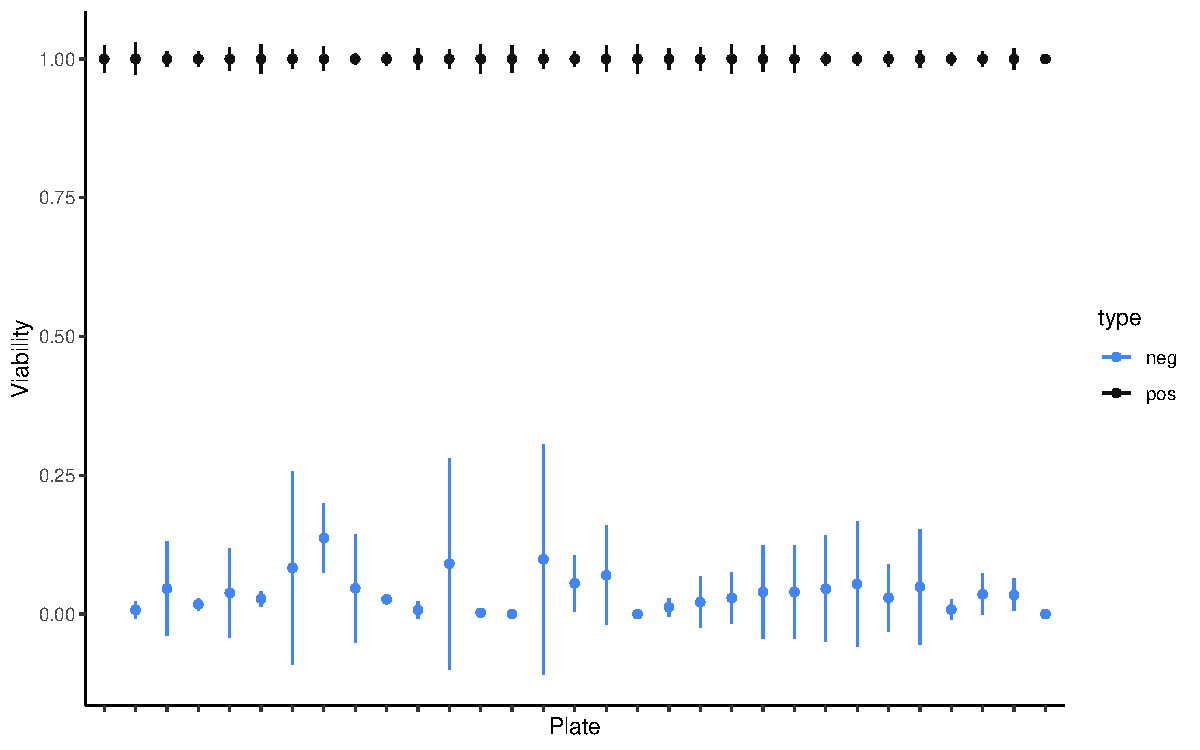
\includegraphics{mofa_exploration_files/figure-latex/unnamed-chunk-11-1.pdf}

\begin{Shaded}
\begin{Highlighting}[]
\NormalTok{gg_f12 <-}\StringTok{ }\NormalTok{weights }\OperatorTok\StringTok{ }
\StringTok{  }\NormalTok{dplyr}\OperatorTok{::}\KeywordTok{rename}\NormalTok{(}\DataTypeTok{line =}\NormalTok{ id) }\OperatorTok
\StringTok{  }\KeywordTok{left_join}\NormalTok{(organoid_size_fit }\OperatorTok\StringTok{ }\KeywordTok{mutate}\NormalTok{(}\DataTypeTok{line =} \KeywordTok{paste0}\NormalTok{(line, }\StringTok{"_"}\NormalTok{, rep))) }\OperatorTok
\StringTok{  }\KeywordTok{left_join}\NormalTok{(organoid_morphology }\OperatorTok\StringTok{ }
\StringTok{            }\KeywordTok{mutate}\NormalTok{(}\DataTypeTok{line =} \KeywordTok{substr}\NormalTok{(line, }\DecValTok{1}\NormalTok{, }\DecValTok{4}\NormalTok{)) }\OperatorTok\StringTok{ }
\StringTok{  }\KeywordTok{expand_grid}\NormalTok{(., }\DataTypeTok{rep =} \KeywordTok{c}\NormalTok{(}\StringTok{"r1"}\NormalTok{, }\StringTok{"r2"}\NormalTok{)) }\OperatorTok\StringTok{ }
\StringTok{  }\KeywordTok{mutate}\NormalTok{(}\DataTypeTok{sample =} \KeywordTok{paste0}\NormalTok{(line, }\StringTok{"_"}\NormalTok{, rep)) }\OperatorTok\StringTok{ }\NormalTok{dplyr}\OperatorTok{::}\KeywordTok{select}\NormalTok{(}\OperatorTok{-}\NormalTok{line, }\DataTypeTok{line =}\NormalTok{ sample)) }\OperatorTok
\StringTok{  }\KeywordTok{distinct}\NormalTok{() }\OperatorTok
\StringTok{  }\KeywordTok{ggplot}\NormalTok{(}\KeywordTok{aes}\NormalTok{(factor1, factor2, }\DataTypeTok{label =}\NormalTok{ line, }\DataTypeTok{color =}\NormalTok{ size, }\DataTypeTok{shape =}\NormalTok{ morphology)) }\OperatorTok{+}\StringTok{ }
\StringTok{  }\KeywordTok{geom_point}\NormalTok{(}\DataTypeTok{size =} \DecValTok{4}\NormalTok{) }\OperatorTok{+}\StringTok{ }
\StringTok{  }\NormalTok{ggrepel}\OperatorTok{::}\KeywordTok{geom_text_repel}\NormalTok{(}\DataTypeTok{color =} \StringTok{"black"}\NormalTok{) }\OperatorTok{+}\StringTok{ }
\StringTok{  }\KeywordTok{scale_color_viridis_c}\NormalTok{() }\OperatorTok{+}\StringTok{ }
\StringTok{  }\KeywordTok{theme_cowplot}\NormalTok{() }\OperatorTok{+}\StringTok{ }
\StringTok{  }\KeywordTok{coord_fixed}\NormalTok{()}
\end{Highlighting}
\end{Shaded}

\begin{verbatim}
## Joining, by = "line"
\end{verbatim}

\begin{verbatim}
## Joining, by = c("line", "rep")
\end{verbatim}

\begin{Shaded}
\begin{Highlighting}[]
\NormalTok{gg_f12 }\OperatorTok{+}\StringTok{ }\KeywordTok{ggsave}\NormalTok{(}\KeywordTok{here}\NormalTok{(}\StringTok{"reports/figures/mofa/factor_12_plot.pdf"}\NormalTok{), }\DataTypeTok{height =} \DecValTok{6}\NormalTok{ , }\DataTypeTok{width =} \DecValTok{6}\NormalTok{)}
\end{Highlighting}
\end{Shaded}

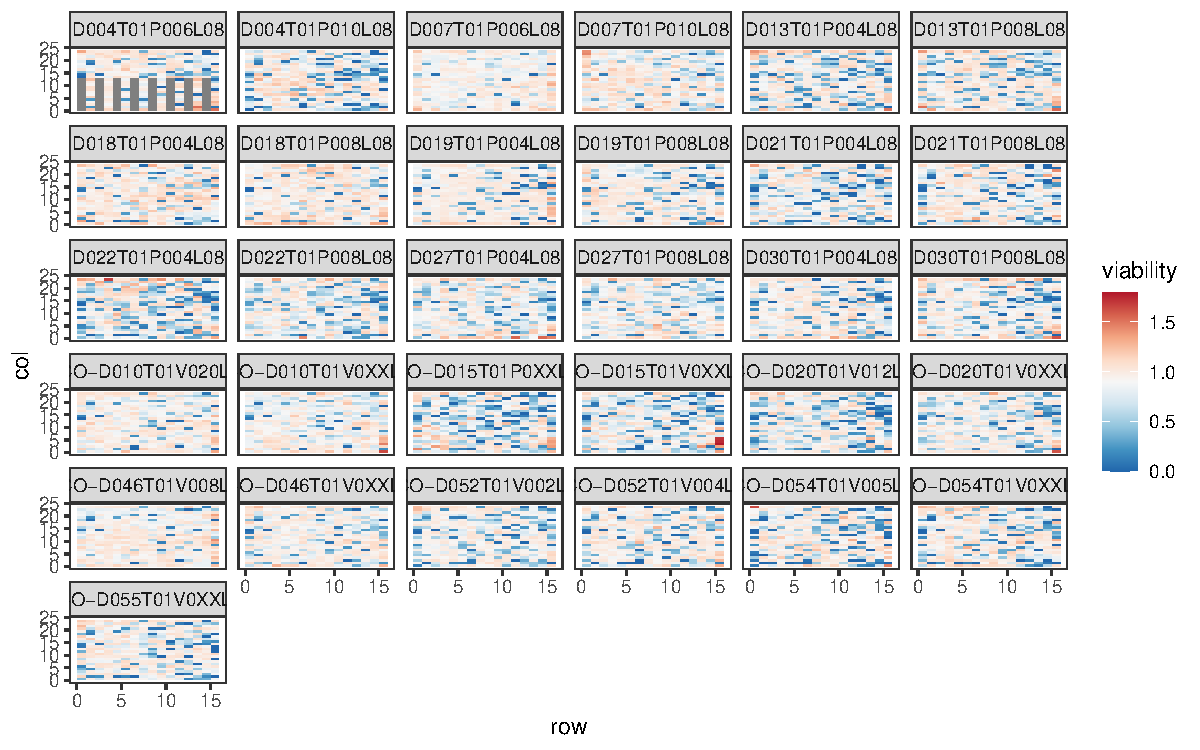
\includegraphics{mofa_exploration_files/figure-latex/unnamed-chunk-12-1.pdf}

\begin{Shaded}
\begin{Highlighting}[]
\NormalTok{gg_f23 <-}\StringTok{ }\NormalTok{weights }\OperatorTok\StringTok{ }
\StringTok{  }\NormalTok{dplyr}\OperatorTok{::}\KeywordTok{rename}\NormalTok{(}\DataTypeTok{line =}\NormalTok{ id) }\OperatorTok
\StringTok{  }\KeywordTok{left_join}\NormalTok{(organoid_size_fit }\OperatorTok\StringTok{ }\KeywordTok{mutate}\NormalTok{(}\DataTypeTok{line =} \KeywordTok{paste0}\NormalTok{(line, }\StringTok{"_"}\NormalTok{, rep))) }\OperatorTok
\StringTok{  }\KeywordTok{ggplot}\NormalTok{(}\KeywordTok{aes}\NormalTok{(factor1, factor3, }\DataTypeTok{label =}\NormalTok{ line)) }\OperatorTok{+}\StringTok{ }
\StringTok{  }\KeywordTok{geom_point}\NormalTok{(}\DataTypeTok{size =} \DecValTok{2}\NormalTok{) }\OperatorTok{+}\StringTok{ }
\StringTok{  }\NormalTok{ggrepel}\OperatorTok{::}\KeywordTok{geom_text_repel}\NormalTok{(}\DataTypeTok{color =} \StringTok{"black"}\NormalTok{) }\OperatorTok{+}\StringTok{ }
\StringTok{  }\KeywordTok{scale_color_viridis_c}\NormalTok{() }\OperatorTok{+}\StringTok{ }
\StringTok{  }\KeywordTok{theme_cowplot}\NormalTok{() }\OperatorTok{+}\StringTok{ }
\StringTok{    }\KeywordTok{theme_cowplot}\NormalTok{() }\OperatorTok{+}\StringTok{ }
\StringTok{  }\KeywordTok{coord_fixed}\NormalTok{() }
\end{Highlighting}
\end{Shaded}

\begin{verbatim}
## Joining, by = "line"
\end{verbatim}

\begin{Shaded}
\begin{Highlighting}[]
\NormalTok{gg_f23 }\OperatorTok{+}\StringTok{ }\KeywordTok{ggsave}\NormalTok{(}\KeywordTok{here}\NormalTok{(}\StringTok{"reports/figures/mofa/factor_23_plot.pdf"}\NormalTok{), }\DataTypeTok{height =} \DecValTok{5}\NormalTok{ , }\DataTypeTok{width =} \DecValTok{5}\NormalTok{)}
\end{Highlighting}
\end{Shaded}

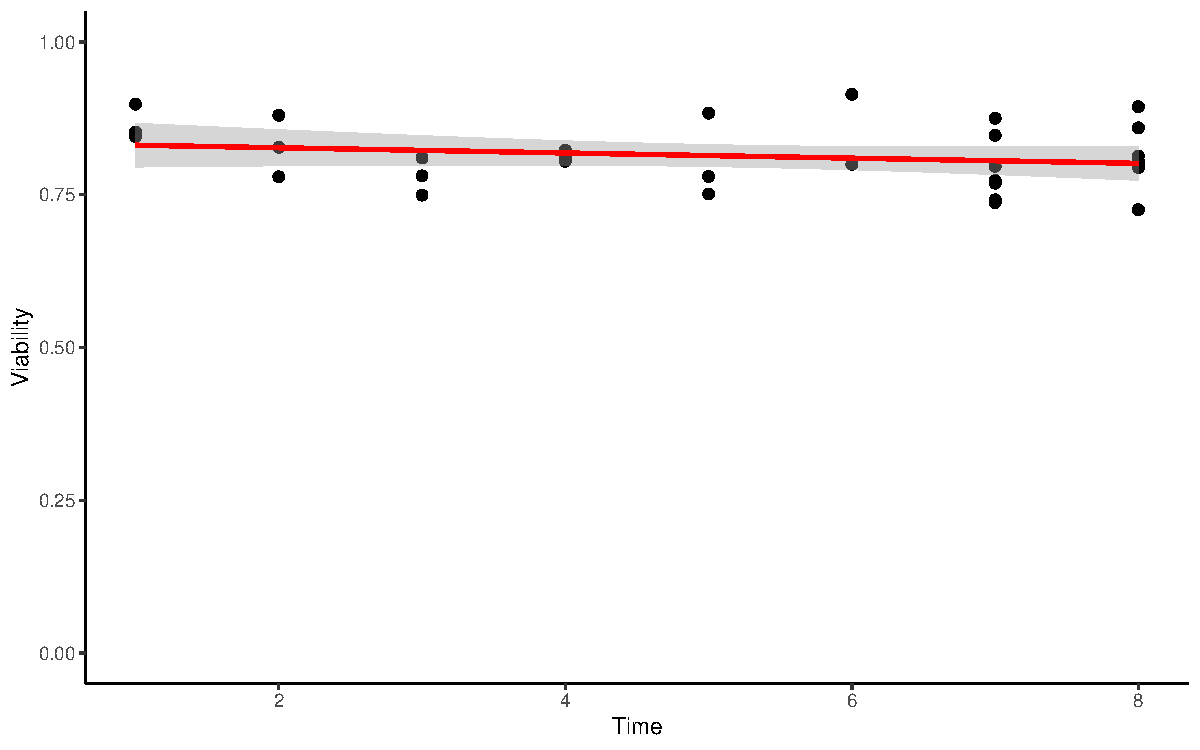
\includegraphics{mofa_exploration_files/figure-latex/unnamed-chunk-13-1.pdf}

\begin{Shaded}
\begin{Highlighting}[]
\NormalTok{cowplot}\OperatorTok{::}\KeywordTok{plot_grid}\NormalTok{(}\KeywordTok{plot_grid}\NormalTok{(gg_ve, gg_ve_feature, gg_f12, }\DataTypeTok{ncol =} \DecValTok{3}\NormalTok{),}
\NormalTok{                   gg_factor_umap,}
                   \DataTypeTok{ncol =} \DecValTok{1}
\NormalTok{                   ) }\OperatorTok{+}\StringTok{ }
\StringTok{  }\KeywordTok{ggsave}\NormalTok{(}\KeywordTok{here}\NormalTok{(}\StringTok{"reports/figures/mofa/mofa_overview.pdf"}\NormalTok{), }\DataTypeTok{height =} \DecValTok{10}\NormalTok{ , }\DataTypeTok{width =} \DecValTok{15}\NormalTok{)}
\end{Highlighting}
\end{Shaded}

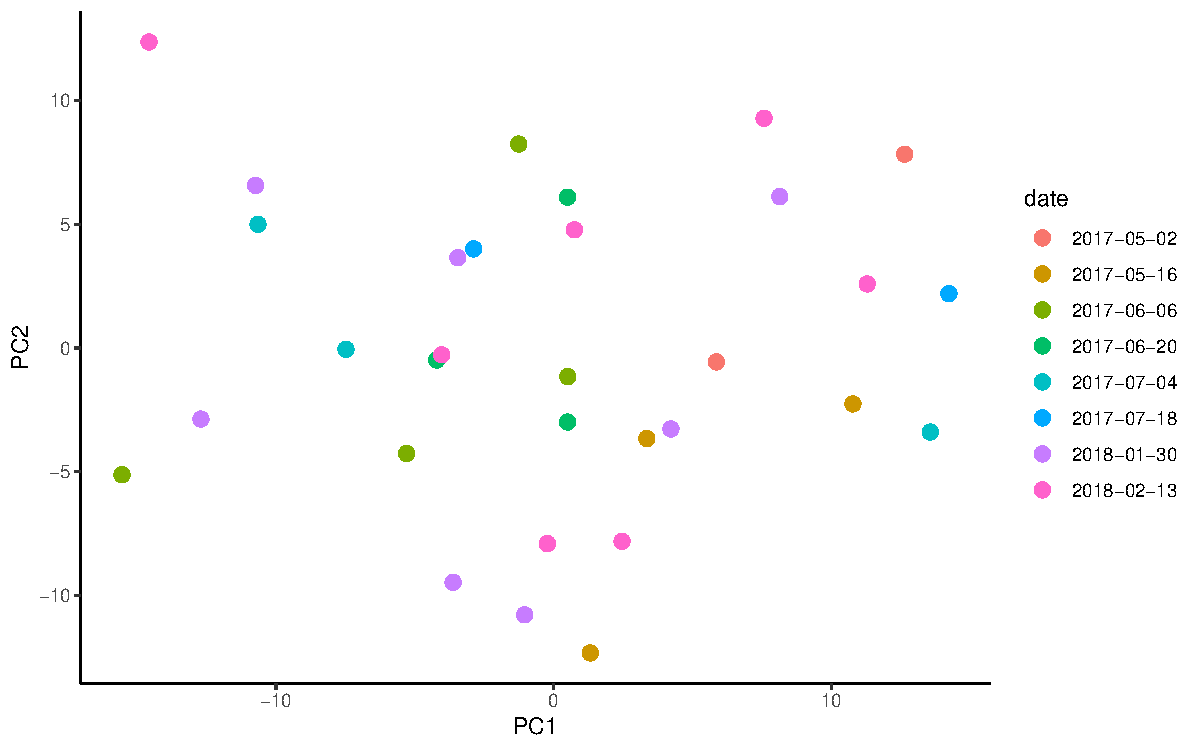
\includegraphics{mofa_exploration_files/figure-latex/unnamed-chunk-14-1.pdf}

\hypertarget{mutations}{%
\subsection{mutations}\label{mutations}}

\begin{Shaded}
\begin{Highlighting}[]
\NormalTok{loadings_mutation }\OperatorTok
\StringTok{  }\KeywordTok{column_to_rownames}\NormalTok{(}\StringTok{"id"}\NormalTok{) }\OperatorTok\StringTok{ }
\StringTok{  }\NormalTok{pheatmap}\OperatorTok{::}\KeywordTok{pheatmap}\NormalTok{()}
\end{Highlighting}
\end{Shaded}

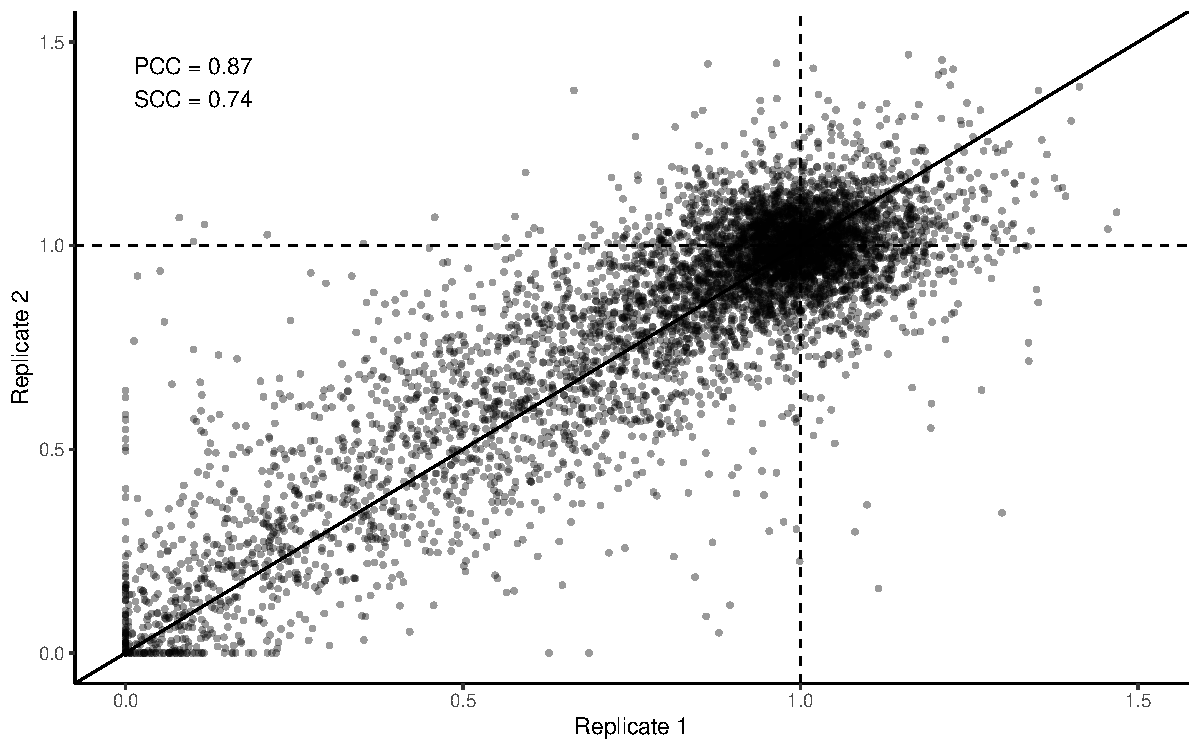
\includegraphics{mofa_exploration_files/figure-latex/unnamed-chunk-15-1.pdf}

\begin{Shaded}
\begin{Highlighting}[]
\NormalTok{df <-}\StringTok{ }\NormalTok{loadings_mutation }\OperatorTok\StringTok{ }
\StringTok{  }\KeywordTok{gather}\NormalTok{(}\DataTypeTok{key =} \StringTok{"factor"}\NormalTok{, }\DataTypeTok{value =} \StringTok{"weight"}\NormalTok{, }\OperatorTok{-}\NormalTok{id) }

\NormalTok{df }\OperatorTok
\StringTok{  }\KeywordTok{ggplot}\NormalTok{(}\KeywordTok{aes}\NormalTok{(factor, weight, }\DataTypeTok{label =}\NormalTok{ id)) }\OperatorTok{+}
\StringTok{  }\KeywordTok{geom_point}\NormalTok{() }\OperatorTok{+}\StringTok{ }
\StringTok{  }\KeywordTok{theme_cowplot}\NormalTok{() }\OperatorTok{+}\StringTok{ }
\StringTok{  }\NormalTok{ggrepel}\OperatorTok{::}\KeywordTok{geom_text_repel}\NormalTok{(}\DataTypeTok{data =}\NormalTok{ df }\OperatorTok\StringTok{ }\KeywordTok{filter}\NormalTok{(id }\OperatorTok\StringTok{ }\KeywordTok{c}\NormalTok{(}\StringTok{"NRAS"}\NormalTok{, }\StringTok{"ERBB2"}\NormalTok{, }\StringTok{"PTEN"}\NormalTok{, }\StringTok{"KRAS"}\NormalTok{, }\StringTok{"PIK3CA"}\NormalTok{)))}
\end{Highlighting}
\end{Shaded}

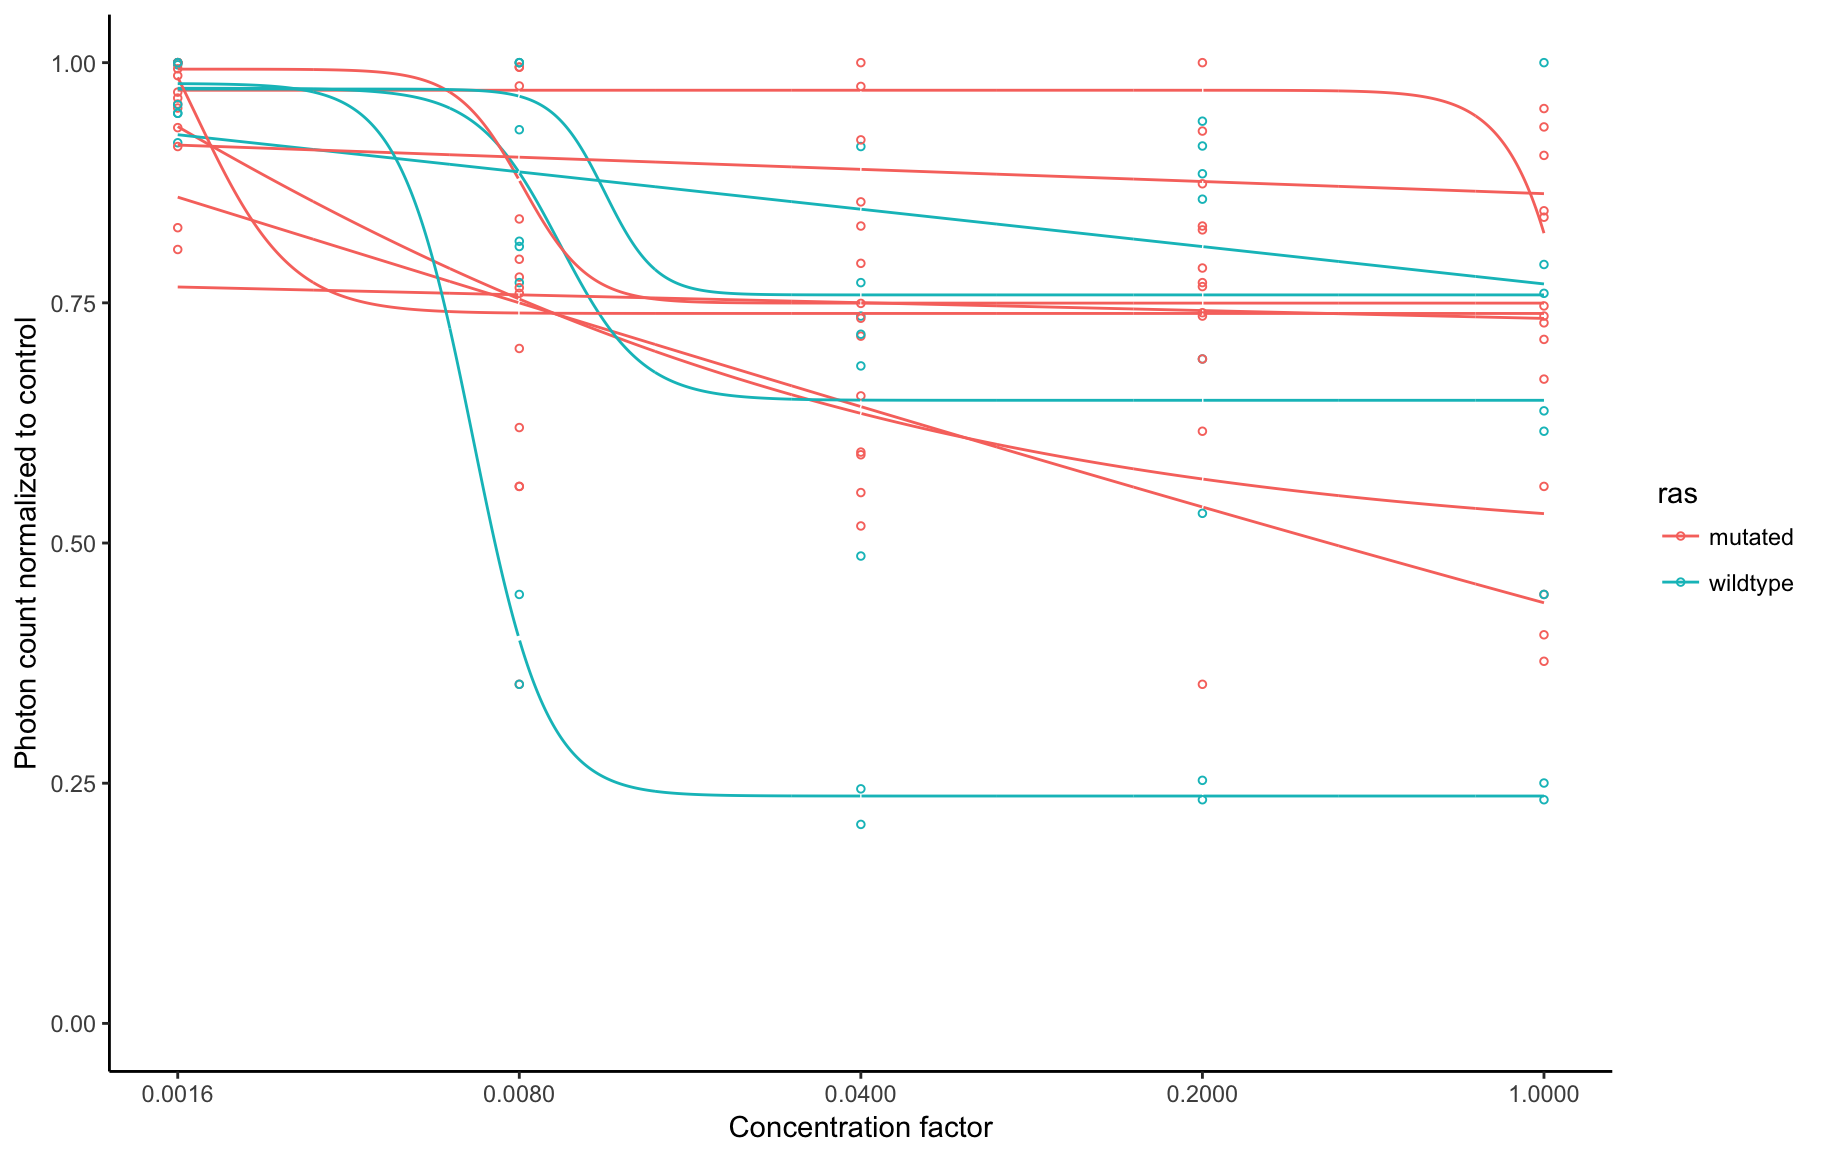
\includegraphics{mofa_exploration_files/figure-latex/unnamed-chunk-16-1.pdf}

\hypertarget{drug-response}{%
\subsection{drug response}\label{drug-response}}

\begin{Shaded}
\begin{Highlighting}[]
\CommentTok{## load drug annotation}
\NormalTok{drug_anno <-}\StringTok{ }\NormalTok{readxl}\OperatorTok{::}\KeywordTok{read_excel}\NormalTok{(here}\OperatorTok{::}\KeywordTok{here}\NormalTok{(}\StringTok{'references/layouts/Compound_Annotation_Libraries_New.xlsx'}\NormalTok{)) }\OperatorTok\StringTok{ }\KeywordTok{distinct}\NormalTok{(}\DataTypeTok{drug =} \StringTok{`}\DataTypeTok{Compound name}\StringTok{`}\NormalTok{, }\DataTypeTok{target =} \StringTok{`}\DataTypeTok{Primary Target}\StringTok{`}\NormalTok{)}

\NormalTok{loadings_drug_activity_tidy <-}\StringTok{ }\NormalTok{loadings_drug_activity }\OperatorTok\StringTok{ }
\StringTok{  }\KeywordTok{mutate}\NormalTok{(}\DataTypeTok{drug =} \KeywordTok{substr}\NormalTok{(id, }\DecValTok{7}\NormalTok{, }\KeywordTok{nchar}\NormalTok{(.))) }\OperatorTok\StringTok{ }
\StringTok{  }\NormalTok{dplyr}\OperatorTok{::}\KeywordTok{select}\NormalTok{(}\OperatorTok{-}\NormalTok{id) }\OperatorTok\StringTok{ }
\StringTok{  }\KeywordTok{arrange}\NormalTok{(}\KeywordTok{desc}\NormalTok{(factor1)) }\OperatorTok\StringTok{ }
\StringTok{  }\KeywordTok{left_join}\NormalTok{(drug_anno)}
\end{Highlighting}
\end{Shaded}

\begin{verbatim}
## Joining, by = "drug"
\end{verbatim}

\begin{Shaded}
\begin{Highlighting}[]
\CommentTok{# }
\CommentTok{# top_n <- 20}
\CommentTok{# }
\CommentTok{# top_drugs <- rbind(}
\CommentTok{#   loadings_drug_activity_tidy %>% arrange(factor1) %>% head(top_n),}
\CommentTok{#   loadings_drug_activity_tidy %>% arrange(factor1) %>% tail(top_n),}
\CommentTok{#   loadings_drug_activity_tidy %>% arrange(factor2) %>% head(top_n),}
\CommentTok{#   loadings_drug_activity_tidy %>% arrange(factor2) %>% tail(top_n),}
\CommentTok{#   loadings_drug_activity_tidy %>% arrange(factor3) %>% head(top_n),}
\CommentTok{#   loadings_drug_activity_tidy %>% arrange(factor3) %>% tail(top_n)}
\CommentTok{# ) %>% distinct()}
\CommentTok{# }
\CommentTok{# top_drugs %>% }
\CommentTok{#   column_to_rownames("drug") %>% }
\CommentTok{#   pheatmap::pheatmap()}
\end{Highlighting}
\end{Shaded}

\begin{Shaded}
\begin{Highlighting}[]
\NormalTok{df <-}\StringTok{ }\NormalTok{loadings_drug_activity_tidy }\OperatorTok\StringTok{ }\NormalTok{dplyr}\OperatorTok{::}\KeywordTok{select}\NormalTok{(}\OperatorTok{-}\NormalTok{target) }\OperatorTok\StringTok{ }
\StringTok{  }\KeywordTok{gather}\NormalTok{(factor_name, value, }\OperatorTok{-}\NormalTok{drug) }\OperatorTok\StringTok{ }
\StringTok{  }\KeywordTok{distinct}\NormalTok{() }

\NormalTok{row_anno <-}\StringTok{  }\NormalTok{df }\OperatorTok\StringTok{ }\KeywordTok{left_join}\NormalTok{(loadings_drug_activity_tidy) }\OperatorTok\StringTok{ }\NormalTok{dplyr}\OperatorTok{::}\KeywordTok{select}\NormalTok{(drug, target) }\OperatorTok
\StringTok{  }\KeywordTok{mutate}\NormalTok{(}\DataTypeTok{id =} \KeywordTok{paste0}\NormalTok{(drug, }\StringTok{"_"}\NormalTok{, target)) }\OperatorTok\StringTok{ }\KeywordTok{distinct}\NormalTok{() }\OperatorTok\StringTok{ }\KeywordTok{as.data.frame}\NormalTok{() }\OperatorTok\StringTok{ }\KeywordTok{column_to_rownames}\NormalTok{(}\StringTok{"id"}\NormalTok{) }
\end{Highlighting}
\end{Shaded}

\begin{verbatim}
## Joining, by = "drug"
\end{verbatim}

\begin{Shaded}
\begin{Highlighting}[]
\NormalTok{df }\OperatorTok
\StringTok{  }\KeywordTok{spread}\NormalTok{(drug, value) }\OperatorTok\StringTok{ }
\StringTok{  }\NormalTok{dplyr}\OperatorTok{::}\KeywordTok{select}\NormalTok{(}\OperatorTok{-}\NormalTok{factor_name) }\OperatorTok
\StringTok{  }\KeywordTok{cor}\NormalTok{() }\OperatorTok\StringTok{ }
\StringTok{  }\KeywordTok{as.matrix}\NormalTok{() }\OperatorTok\StringTok{ }
\StringTok{  }\NormalTok{pheatmap}\OperatorTok{::}\KeywordTok{pheatmap}\NormalTok{(}\DataTypeTok{show_rownames =} \OtherTok{FALSE}\NormalTok{, }
                     \DataTypeTok{show_colnames =} \OtherTok{FALSE}\NormalTok{)}
\end{Highlighting}
\end{Shaded}

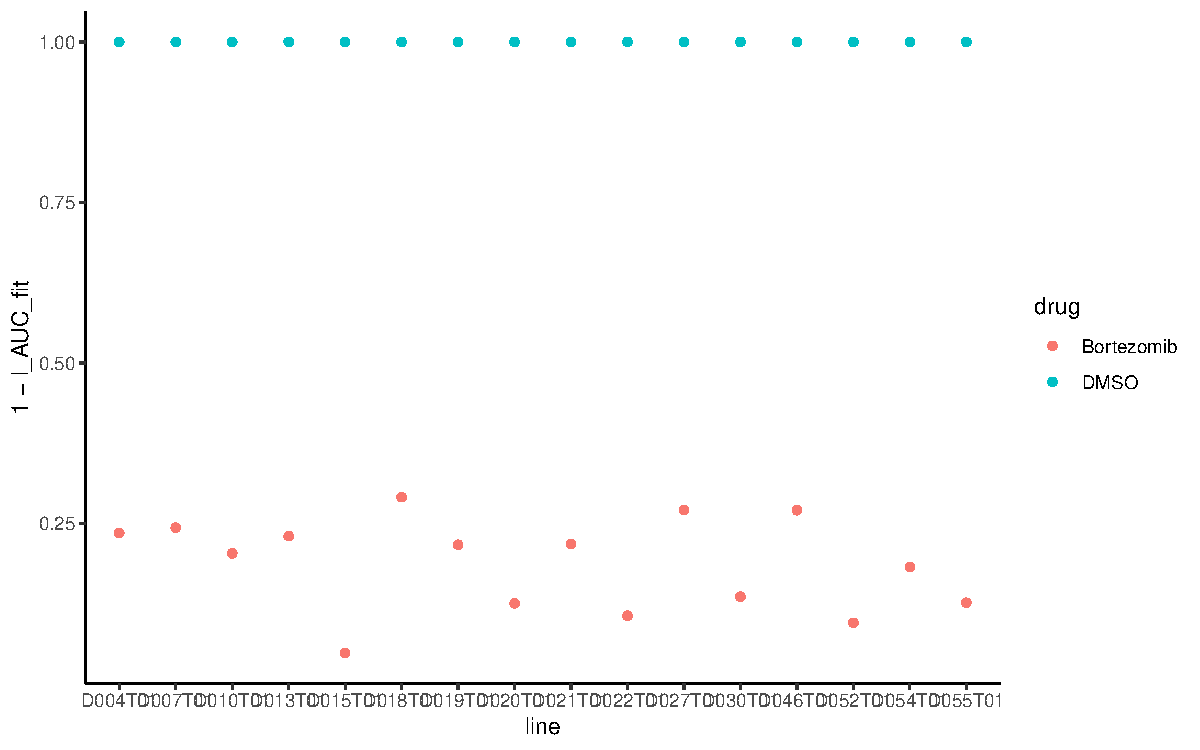
\includegraphics{mofa_exploration_files/figure-latex/unnamed-chunk-18-1.pdf}

\begin{Shaded}
\begin{Highlighting}[]
\NormalTok{drug_activity_test <-}\StringTok{ }\NormalTok{loadings_drug_activity_tidy }\OperatorTok\StringTok{ }\KeywordTok{semi_join}\NormalTok{(loadings_drug_activity_tidy }\OperatorTok\StringTok{ }
\StringTok{                                            }\NormalTok{dplyr}\OperatorTok{::}\KeywordTok{count}\NormalTok{(target) }\OperatorTok\StringTok{ }
\StringTok{                                            }\KeywordTok{filter}\NormalTok{(n }\OperatorTok{>=}\DecValTok{5}\NormalTok{)) }
\end{Highlighting}
\end{Shaded}

\begin{verbatim}
## Joining, by = "target"
\end{verbatim}

\begin{Shaded}
\begin{Highlighting}[]
\NormalTok{drug_activity_test_result <-}\StringTok{ }\KeywordTok{rbind}\NormalTok{(}
  \KeywordTok{lm}\NormalTok{(factor1 }\OperatorTok{~}\StringTok{ }\NormalTok{target, }\DataTypeTok{data =}\NormalTok{ drug_activity_test) }\OperatorTok\StringTok{ }\KeywordTok{summary}\NormalTok{() }\OperatorTok\StringTok{ }\NormalTok{broom}\OperatorTok{::}\KeywordTok{tidy}\NormalTok{() }\OperatorTok\StringTok{ }\KeywordTok{mutate}\NormalTok{(}\DataTypeTok{factor =} \StringTok{"factor1"}\NormalTok{),}
  \KeywordTok{lm}\NormalTok{(factor2 }\OperatorTok{~}\StringTok{ }\NormalTok{target, }\DataTypeTok{data =}\NormalTok{ drug_activity_test) }\OperatorTok\StringTok{ }\KeywordTok{summary}\NormalTok{() }\OperatorTok\StringTok{ }\NormalTok{broom}\OperatorTok{::}\KeywordTok{tidy}\NormalTok{() }\OperatorTok\StringTok{ }\KeywordTok{mutate}\NormalTok{(}\DataTypeTok{factor =} \StringTok{"factor2"}\NormalTok{),}
  \KeywordTok{lm}\NormalTok{(factor3 }\OperatorTok{~}\StringTok{ }\NormalTok{target, }\DataTypeTok{data =}\NormalTok{ drug_activity_test) }\OperatorTok\StringTok{ }\KeywordTok{summary}\NormalTok{() }\OperatorTok\StringTok{ }\NormalTok{broom}\OperatorTok{::}\KeywordTok{tidy}\NormalTok{() }\OperatorTok\StringTok{ }\KeywordTok{mutate}\NormalTok{(}\DataTypeTok{factor =} \StringTok{"factor3"}\NormalTok{)) }

\NormalTok{df <-}\StringTok{ }\NormalTok{drug_activity_test_result }\OperatorTok\StringTok{ }
\StringTok{  }\KeywordTok{filter}\NormalTok{(term }\OperatorTok{!=}\StringTok{ "(Intercept)"}\NormalTok{) }\OperatorTok\StringTok{ }
\StringTok{  }\NormalTok{dplyr}\OperatorTok{::}\KeywordTok{select}\NormalTok{(term, statistic, factor) }\OperatorTok\StringTok{ }
\StringTok{  }\KeywordTok{mutate}\NormalTok{(}\DataTypeTok{term =} \KeywordTok{substr}\NormalTok{(term, }\DecValTok{7}\NormalTok{, }\KeywordTok{nchar}\NormalTok{(term)))}

\NormalTok{df }\OperatorTok\StringTok{ }
\StringTok{  }\KeywordTok{spread}\NormalTok{(factor, statistic) }\OperatorTok\StringTok{ }
\StringTok{  }\KeywordTok{column_to_rownames}\NormalTok{(}\StringTok{"term"}\NormalTok{) }\OperatorTok\StringTok{ }
\StringTok{  }\NormalTok{pheatmap}\OperatorTok{::}\KeywordTok{pheatmap}\NormalTok{()}
\end{Highlighting}
\end{Shaded}

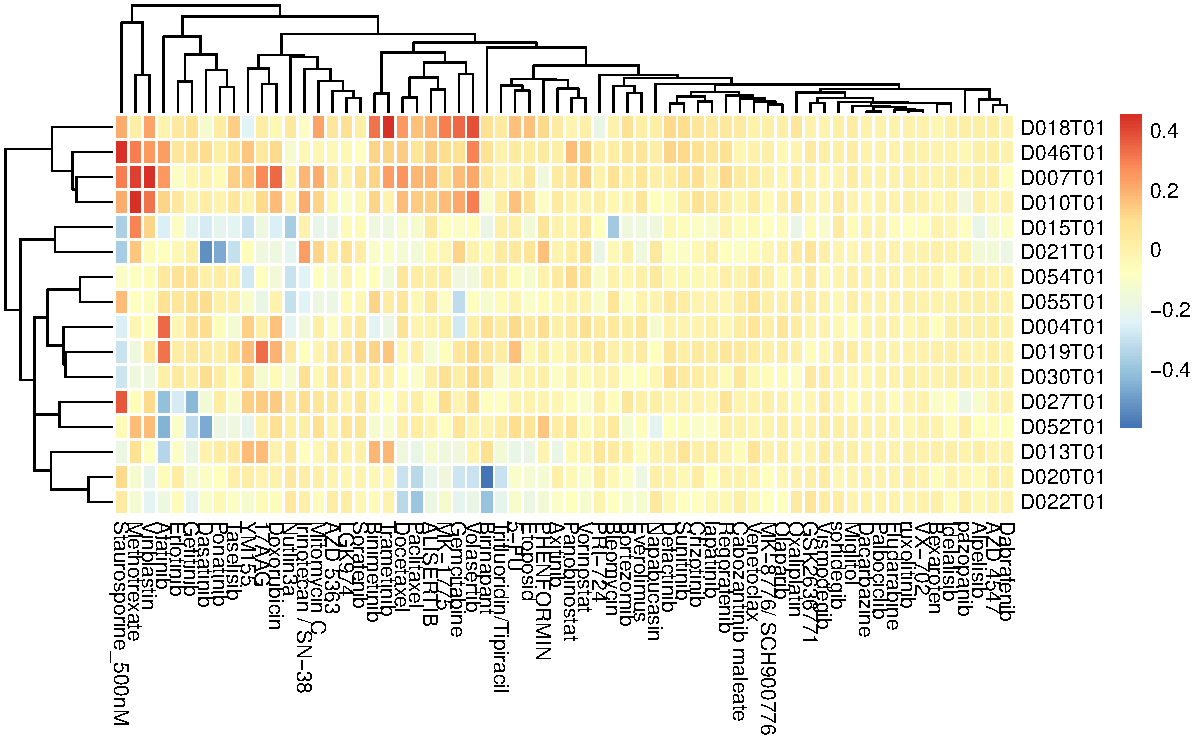
\includegraphics{mofa_exploration_files/figure-latex/unnamed-chunk-20-1.pdf}

\begin{Shaded}
\begin{Highlighting}[]
\NormalTok{drug_activity_test_result }\OperatorTok\StringTok{ }
\StringTok{  }\KeywordTok{mutate}\NormalTok{(}\DataTypeTok{fdr =} \KeywordTok{p.adjust}\NormalTok{(p.value, }\DataTypeTok{method =} \StringTok{"BH"}\NormalTok{)) }\OperatorTok\StringTok{ }
\StringTok{  }\KeywordTok{filter}\NormalTok{(fdr }\OperatorTok{<=}\StringTok{ }\FloatTok{0.2}\NormalTok{) }\OperatorTok\StringTok{ }
\StringTok{  }\KeywordTok{filter}\NormalTok{(term }\OperatorTok{!=}\StringTok{ "(Intercept)"}\NormalTok{) }\OperatorTok\StringTok{ }
\StringTok{  }\KeywordTok{arrange}\NormalTok{(factor, statistic)}
\end{Highlighting}
\end{Shaded}

\begin{verbatim}
## # A tibble: 6 x 7
##   term               estimate std.error statistic      p.value factor        fdr
##   <chr>                 <dbl>     <dbl>     <dbl>        <dbl> <chr>       <dbl>
## 1 targetEGFR           -0.522    0.102      -5.12      8.15e-7 facto~    2.57e-5
## 2 targetMEK            -0.269    0.0956     -2.81      5.46e-3 facto~    6.89e-2
## 3 targetSrc             0.250    0.103       2.42      1.66e-2 facto~    1.68e-1
## 4 targetWnt/beta-ca~    0.353    0.117       3.02      2.95e-3 facto~    4.64e-2
## 5 targetEGFR            0.276    0.0894      3.08      2.40e-3 facto~    4.64e-2
## 6 targetAurora Kina~    0.574    0.0894      6.42      1.25e-9 facto~    7.90e-8
\end{verbatim}

\hypertarget{exporting-factors-loadings-for-enrichment}{%
\subsection{exporting factors loadings for
enrichment}\label{exporting-factors-loadings-for-enrichment}}

\begin{Shaded}
\begin{Highlighting}[]
\CommentTok{# top 100 genes}
\NormalTok{loadings_expression }\OperatorTok\StringTok{ }\KeywordTok{arrange}\NormalTok{(}\KeywordTok{desc}\NormalTok{(factor1)) }\OperatorTok\StringTok{ }\KeywordTok{head}\NormalTok{(}\DecValTok{100}\NormalTok{) }\OperatorTok\StringTok{ }
\StringTok{  }\NormalTok{dplyr}\OperatorTok{::}\KeywordTok{mutate}\NormalTok{(}\DataTypeTok{id =} \KeywordTok{substr}\NormalTok{(id, }\DecValTok{1}\NormalTok{, }\KeywordTok{nchar}\NormalTok{(id)}\OperatorTok{-}\DecValTok{11}\NormalTok{)) }\OperatorTok\StringTok{ }
\StringTok{  }\KeywordTok{arrange}\NormalTok{(}\KeywordTok{desc}\NormalTok{(id)) }\OperatorTok
\StringTok{  }\NormalTok{dplyr}\OperatorTok{::}\KeywordTok{select}\NormalTok{(id) }\OperatorTok\StringTok{ }\KeywordTok{write_csv}\NormalTok{(here}\OperatorTok{::}\KeywordTok{here}\NormalTok{(}\StringTok{"reports/tables/factor1_top.csv"}\NormalTok{))}

\NormalTok{loadings_expression }\OperatorTok\StringTok{ }\KeywordTok{arrange}\NormalTok{(}\KeywordTok{desc}\NormalTok{(factor2)) }\OperatorTok\StringTok{ }\KeywordTok{head}\NormalTok{(}\DecValTok{100}\NormalTok{) }\OperatorTok\StringTok{ }
\StringTok{  }\NormalTok{dplyr}\OperatorTok{::}\KeywordTok{mutate}\NormalTok{(}\DataTypeTok{id =} \KeywordTok{substr}\NormalTok{(id, }\DecValTok{1}\NormalTok{, }\KeywordTok{nchar}\NormalTok{(id)}\OperatorTok{-}\DecValTok{11}\NormalTok{)) }\OperatorTok\StringTok{ }
\StringTok{  }\NormalTok{dplyr}\OperatorTok{::}\KeywordTok{select}\NormalTok{(id) }\OperatorTok\StringTok{ }\KeywordTok{write_csv}\NormalTok{(here}\OperatorTok{::}\KeywordTok{here}\NormalTok{(}\StringTok{"reports/tables/factor2_top.csv"}\NormalTok{))}

\NormalTok{loadings_expression }\OperatorTok\StringTok{ }\KeywordTok{arrange}\NormalTok{(}\KeywordTok{desc}\NormalTok{(factor3)) }\OperatorTok\StringTok{ }\KeywordTok{head}\NormalTok{(}\DecValTok{100}\NormalTok{) }\OperatorTok\StringTok{ }
\StringTok{  }\NormalTok{dplyr}\OperatorTok{::}\KeywordTok{mutate}\NormalTok{(}\DataTypeTok{id =} \KeywordTok{substr}\NormalTok{(id, }\DecValTok{1}\NormalTok{, }\KeywordTok{nchar}\NormalTok{(id)}\OperatorTok{-}\DecValTok{11}\NormalTok{)) }\OperatorTok\StringTok{ }
\StringTok{  }\NormalTok{dplyr}\OperatorTok{::}\KeywordTok{select}\NormalTok{(id) }\OperatorTok\StringTok{ }\KeywordTok{write_csv}\NormalTok{(here}\OperatorTok{::}\KeywordTok{here}\NormalTok{(}\StringTok{"reports/tables/factor3_top.csv"}\NormalTok{))}

\CommentTok{# all genes}
\NormalTok{loadings_expression }\OperatorTok\StringTok{ }\KeywordTok{arrange}\NormalTok{(}\KeywordTok{desc}\NormalTok{(factor1)) }\OperatorTok\StringTok{ }
\StringTok{  }\NormalTok{dplyr}\OperatorTok{::}\KeywordTok{mutate}\NormalTok{(}\DataTypeTok{id =} \KeywordTok{substr}\NormalTok{(id, }\DecValTok{1}\NormalTok{, }\KeywordTok{nchar}\NormalTok{(id)}\OperatorTok{-}\DecValTok{11}\NormalTok{)) }\OperatorTok\StringTok{ }
\StringTok{  }\KeywordTok{arrange}\NormalTok{(}\KeywordTok{desc}\NormalTok{(id)) }\OperatorTok
\StringTok{  }\NormalTok{dplyr}\OperatorTok{::}\KeywordTok{select}\NormalTok{(id, factor1) }\OperatorTok\StringTok{ }\KeywordTok{write_csv}\NormalTok{(here}\OperatorTok{::}\KeywordTok{here}\NormalTok{(}\StringTok{"reports/tables/factor1_all.csv"}\NormalTok{))}

\NormalTok{loadings_expression }\OperatorTok\StringTok{ }\KeywordTok{arrange}\NormalTok{(}\KeywordTok{desc}\NormalTok{(factor2)) }\OperatorTok\StringTok{ }
\StringTok{  }\NormalTok{dplyr}\OperatorTok{::}\KeywordTok{mutate}\NormalTok{(}\DataTypeTok{id =} \KeywordTok{substr}\NormalTok{(id, }\DecValTok{1}\NormalTok{, }\KeywordTok{nchar}\NormalTok{(id)}\OperatorTok{-}\DecValTok{11}\NormalTok{)) }\OperatorTok\StringTok{ }
\StringTok{  }\NormalTok{dplyr}\OperatorTok{::}\KeywordTok{select}\NormalTok{(id, factor2) }\OperatorTok\StringTok{ }\KeywordTok{write_csv}\NormalTok{(here}\OperatorTok{::}\KeywordTok{here}\NormalTok{(}\StringTok{"reports/tables/factor2_all.csv"}\NormalTok{))}

\NormalTok{loadings_expression }\OperatorTok\StringTok{ }\KeywordTok{arrange}\NormalTok{(}\KeywordTok{desc}\NormalTok{(factor3)) }\OperatorTok\StringTok{ }
\StringTok{  }\NormalTok{dplyr}\OperatorTok{::}\KeywordTok{mutate}\NormalTok{(}\DataTypeTok{id =} \KeywordTok{substr}\NormalTok{(id, }\DecValTok{1}\NormalTok{, }\KeywordTok{nchar}\NormalTok{(id)}\OperatorTok{-}\DecValTok{11}\NormalTok{)) }\OperatorTok\StringTok{ }
\StringTok{  }\NormalTok{dplyr}\OperatorTok{::}\KeywordTok{select}\NormalTok{(id, factor3) }\OperatorTok\StringTok{ }\KeywordTok{write_csv}\NormalTok{(here}\OperatorTok{::}\KeywordTok{here}\NormalTok{(}\StringTok{"reports/tables/factor3_all.csv"}\NormalTok{))}
\end{Highlighting}
\end{Shaded}

\hypertarget{factor-1}{%
\section{factor 1}\label{factor-1}}

\hypertarget{size}{%
\subsection{size}\label{size}}

\begin{Shaded}
\begin{Highlighting}[]
\NormalTok{gg_sizef1 <-}\StringTok{ }\NormalTok{weights }\OperatorTok\StringTok{ }
\StringTok{  }\NormalTok{dplyr}\OperatorTok{::}\KeywordTok{rename}\NormalTok{(}\DataTypeTok{line =}\NormalTok{ id) }\OperatorTok
\StringTok{  }\KeywordTok{left_join}\NormalTok{(organoid_size_fit }\OperatorTok\StringTok{ }\KeywordTok{mutate}\NormalTok{(}\DataTypeTok{line =} \KeywordTok{paste0}\NormalTok{(line, }\StringTok{"_"}\NormalTok{, rep))) }\OperatorTok
\StringTok{  }\KeywordTok{left_join}\NormalTok{(organoid_morphology }\OperatorTok\StringTok{ }
\StringTok{            }\KeywordTok{mutate}\NormalTok{(}\DataTypeTok{line =} \KeywordTok{substr}\NormalTok{(line, }\DecValTok{1}\NormalTok{, }\DecValTok{4}\NormalTok{)) }\OperatorTok\StringTok{ }
\StringTok{  }\KeywordTok{expand_grid}\NormalTok{(., }\DataTypeTok{rep =} \KeywordTok{c}\NormalTok{(}\StringTok{"r1"}\NormalTok{, }\StringTok{"r2"}\NormalTok{)) }\OperatorTok\StringTok{ }
\StringTok{  }\KeywordTok{mutate}\NormalTok{(}\DataTypeTok{sample =} \KeywordTok{paste0}\NormalTok{(line, }\StringTok{"_"}\NormalTok{, rep)) }\OperatorTok\StringTok{ }\NormalTok{dplyr}\OperatorTok{::}\KeywordTok{select}\NormalTok{(}\OperatorTok{-}\NormalTok{line, }\DataTypeTok{line =}\NormalTok{ sample)) }\OperatorTok
\StringTok{  }\KeywordTok{distinct}\NormalTok{() }\OperatorTok
\StringTok{  }\KeywordTok{ggplot}\NormalTok{(}\KeywordTok{aes}\NormalTok{(factor1, size, }\DataTypeTok{label =}\NormalTok{ line)) }\OperatorTok{+}\StringTok{ }
\StringTok{  }\KeywordTok{geom_smooth}\NormalTok{(}\DataTypeTok{method =} \StringTok{"lm"}\NormalTok{, }\DataTypeTok{se =} \OtherTok{FALSE}\NormalTok{, }\DataTypeTok{color =} \StringTok{"grey"}\NormalTok{) }\OperatorTok{+}
\StringTok{  }\KeywordTok{geom_point}\NormalTok{(}\DataTypeTok{size =} \DecValTok{2}\NormalTok{) }\OperatorTok{+}\StringTok{ }
\StringTok{  }\NormalTok{ggrepel}\OperatorTok{::}\KeywordTok{geom_text_repel}\NormalTok{(}\DataTypeTok{color =} \StringTok{"black"}\NormalTok{) }\OperatorTok{+}\StringTok{ }
\StringTok{  }\KeywordTok{scale_color_viridis_c}\NormalTok{() }\OperatorTok{+}\StringTok{ }
\StringTok{  }\KeywordTok{labs}\NormalTok{(}\DataTypeTok{y =} \StringTok{"expected size"}\NormalTok{) }\OperatorTok{+}
\StringTok{  }\KeywordTok{theme_cowplot}\NormalTok{() }\OperatorTok{+}\StringTok{ }
\StringTok{  }\KeywordTok{coord_fixed}\NormalTok{(}\DataTypeTok{ratio =} \DecValTok{2}\NormalTok{)}
\end{Highlighting}
\end{Shaded}

\begin{verbatim}
## Joining, by = "line"
\end{verbatim}

\begin{verbatim}
## Joining, by = c("line", "rep")
\end{verbatim}

\begin{Shaded}
\begin{Highlighting}[]
\NormalTok{gg_sizef1 }\OperatorTok{+}\StringTok{ }\KeywordTok{ggsave}\NormalTok{(here}\OperatorTok{::}\KeywordTok{here}\NormalTok{(}\StringTok{"reports/figures/mofa/f1_size.pdf"}\NormalTok{), }\DataTypeTok{width =} \DecValTok{5}\NormalTok{, }\DataTypeTok{height =} \DecValTok{5}\NormalTok{)}
\end{Highlighting}
\end{Shaded}

\begin{verbatim}
## `geom_smooth()` using formula 'y ~ x'
\end{verbatim}

\begin{verbatim}
## `geom_smooth()` using formula 'y ~ x'
\end{verbatim}

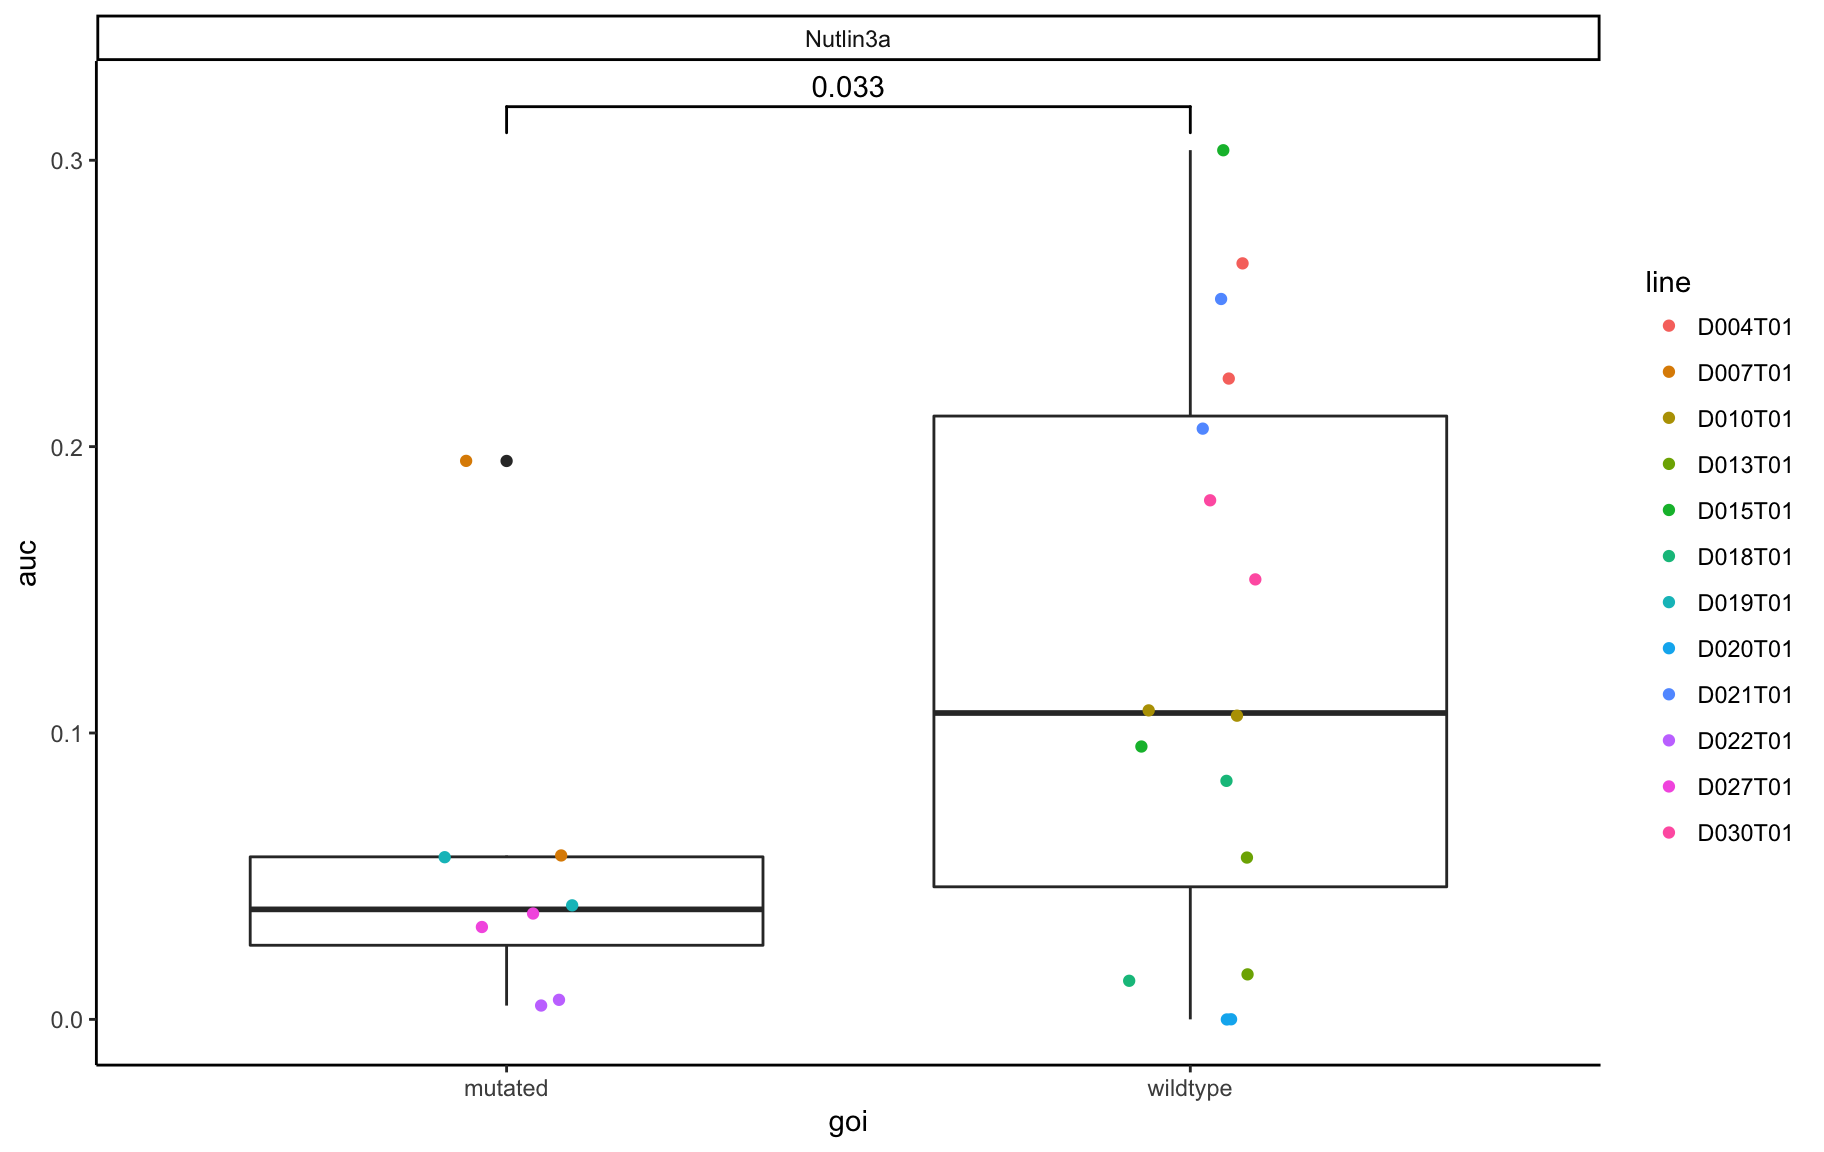
\includegraphics{mofa_exploration_files/figure-latex/unnamed-chunk-23-1.pdf}

\hypertarget{gene-expression}{%
\subsection{gene expression}\label{gene-expression}}

\begin{Shaded}
\begin{Highlighting}[]
\NormalTok{gg_f1_geneexp <-}\StringTok{ }\KeywordTok{plot_weights}\NormalTok{(model,}
  \DataTypeTok{view =} \StringTok{"expression"}\NormalTok{,}
  \DataTypeTok{factor =} \DecValTok{1}\NormalTok{,}
  \DataTypeTok{nfeatures =} \DecValTok{10}\NormalTok{,     }\CommentTok{# Number of features to highlight}
  \DataTypeTok{scale =}\NormalTok{ T,          }\CommentTok{# Scale weights from -1 to 1}
  \DataTypeTok{abs =}\NormalTok{ F             }\CommentTok{# Take the absolute value?}
\NormalTok{) }\OperatorTok{+}\StringTok{ }
\StringTok{  }\KeywordTok{theme_cowplot}\NormalTok{() }\OperatorTok{+}\StringTok{ }
\StringTok{  }\KeywordTok{theme}\NormalTok{(}\DataTypeTok{axis.text.y =} \KeywordTok{element_blank}\NormalTok{(),}
        \DataTypeTok{axis.ticks.y =}\KeywordTok{element_blank}\NormalTok{()) }
\end{Highlighting}
\end{Shaded}

\begin{verbatim}
## Warning: Ignoring unknown parameters: max.overlaps
\end{verbatim}

\begin{Shaded}
\begin{Highlighting}[]
\NormalTok{gg_f1_geneexp }\OperatorTok{+}\StringTok{ }
\StringTok{  }\KeywordTok{ggsave}\NormalTok{(here}\OperatorTok{::}\KeywordTok{here}\NormalTok{(}\StringTok{"reports/figures/mofa/f1_genexp.pdf"}\NormalTok{), }\DataTypeTok{width =} \DecValTok{4}\NormalTok{, }\DataTypeTok{height =} \DecValTok{4}\NormalTok{)}
\end{Highlighting}
\end{Shaded}

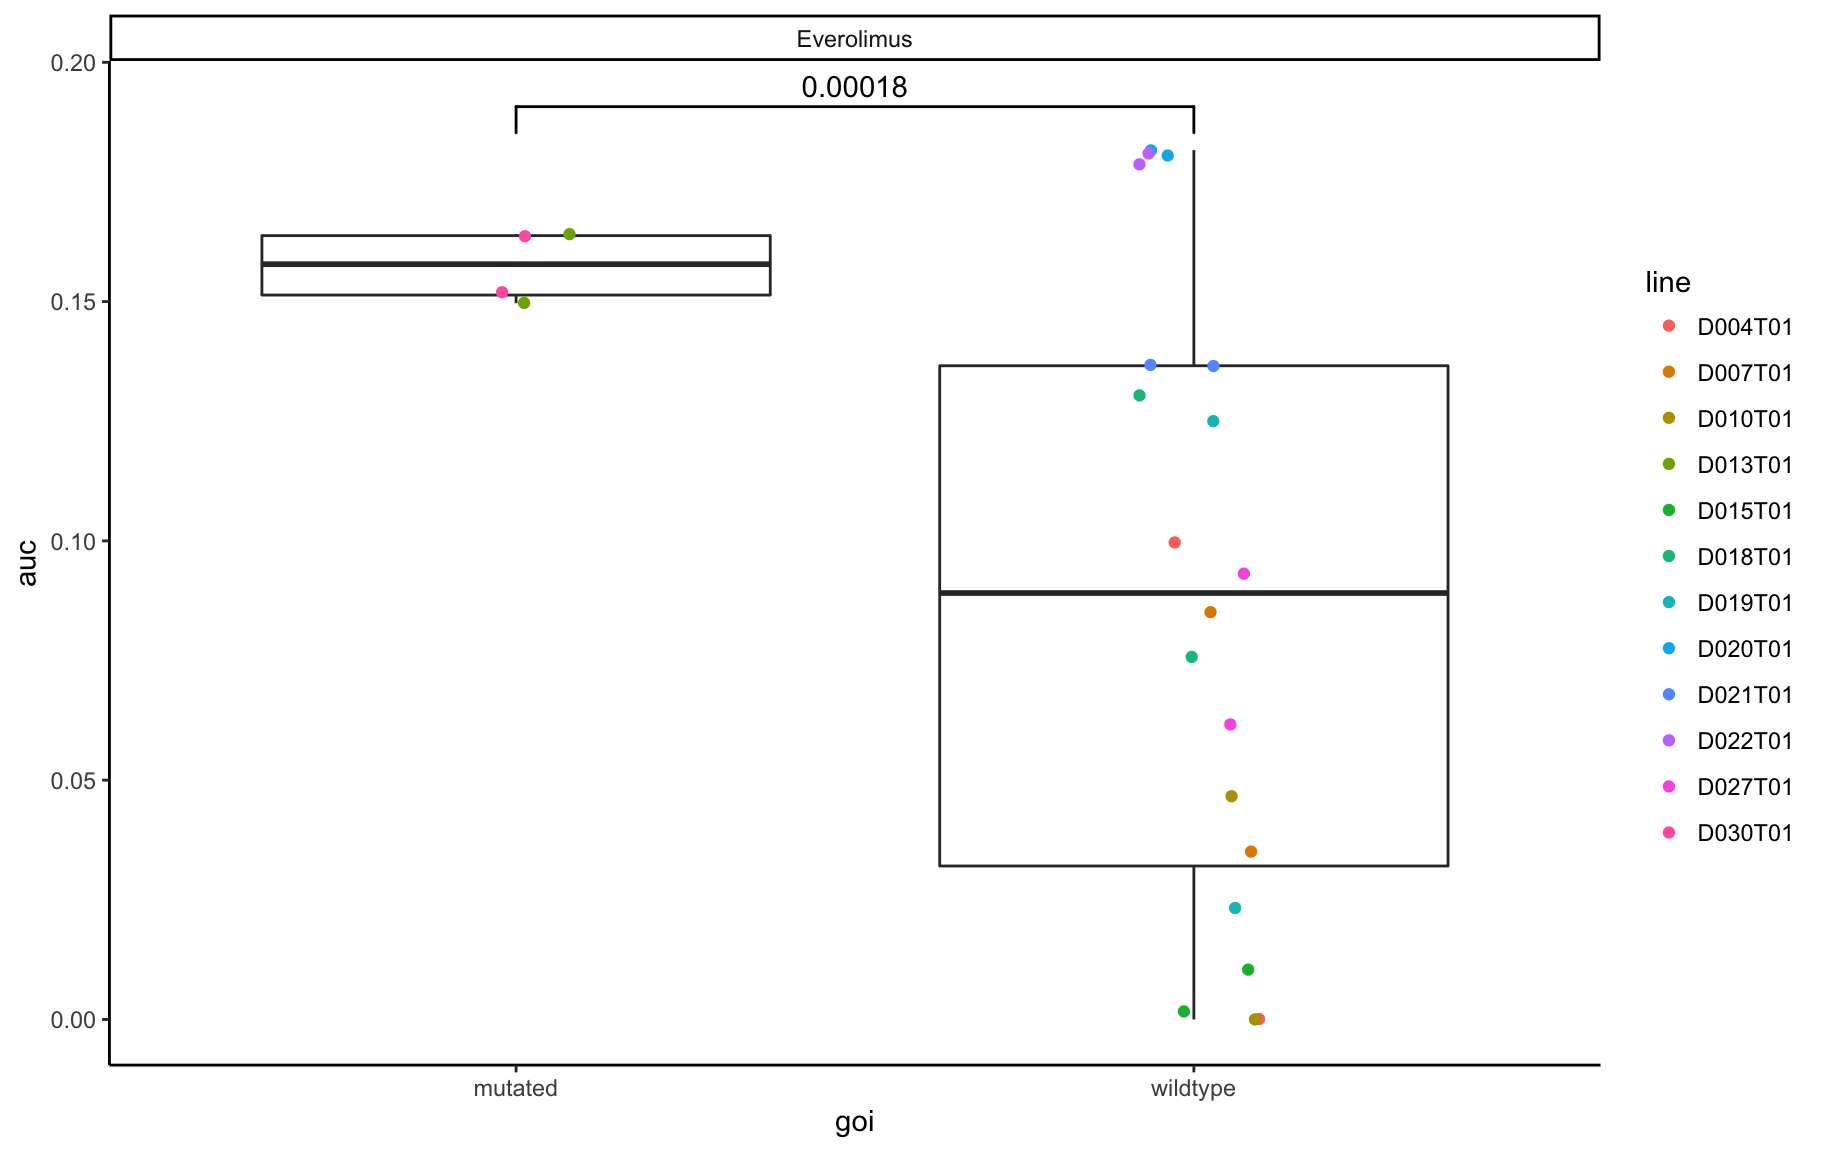
\includegraphics{mofa_exploration_files/figure-latex/unnamed-chunk-24-1.pdf}
growth control via IGF signaling cell adhesion via FYN signaling, high
fibronectin expression DLX- TGFb and BMP inhibiting transcription factor

\begin{Shaded}
\begin{Highlighting}[]
\NormalTok{df <-}\StringTok{ }\NormalTok{loadings_expression }\OperatorTok\StringTok{ }
\StringTok{  }\KeywordTok{separate}\NormalTok{(id, }\KeywordTok{c}\NormalTok{(}\StringTok{"symbol"}\NormalTok{), }\DataTypeTok{sep =} \StringTok{"_exp"}\NormalTok{) }\OperatorTok\StringTok{ }
\StringTok{  }\KeywordTok{filter}\NormalTok{(symbol }\OperatorTok{!=}\StringTok{ ""}\NormalTok{) }\OperatorTok
\StringTok{  }\KeywordTok{left_join}\NormalTok{(promise_long_filtered_top }\OperatorTok\StringTok{ }\NormalTok{dplyr}\OperatorTok{::}\KeywordTok{select}\NormalTok{(symbol, entrez) }\OperatorTok\StringTok{ }\KeywordTok{distinct}\NormalTok{()) }\OperatorTok
\StringTok{  }\KeywordTok{arrange}\NormalTok{(}\KeywordTok{desc}\NormalTok{(factor1)) }\OperatorTok
\StringTok{  }\KeywordTok{mutate}\NormalTok{(}\DataTypeTok{order =} \KeywordTok{nrow}\NormalTok{(.)}\OperatorTok{:}\DecValTok{1}\NormalTok{)}
\end{Highlighting}
\end{Shaded}

\begin{verbatim}
## Warning: Expected 1 pieces. Additional pieces discarded in 3222 rows [1, 2, 3,
## 4, 5, 6, 7, 8, 9, 10, 11, 12, 13, 14, 15, 16, 17, 18, 19, 20, ...].
\end{verbatim}

\begin{verbatim}
## Joining, by = "symbol"
\end{verbatim}

\begin{Shaded}
\begin{Highlighting}[]
\NormalTok{df }\OperatorTok\StringTok{ }
\StringTok{  }\KeywordTok{ggplot}\NormalTok{(}\KeywordTok{aes}\NormalTok{(order, factor1)) }\OperatorTok{+}\StringTok{ }
\StringTok{  }\KeywordTok{geom_point}\NormalTok{()}\OperatorTok{+}\StringTok{ }
\StringTok{  }\KeywordTok{geom_point}\NormalTok{(}\DataTypeTok{data =}\NormalTok{ df }\OperatorTok\StringTok{ }\KeywordTok{filter}\NormalTok{(symbol }\OperatorTok\StringTok{ }\KeywordTok{c}\NormalTok{(}\StringTok{"H19"}\NormalTok{, }\StringTok{"IGF2"}\NormalTok{)), }
             \DataTypeTok{color =} \StringTok{"blue"}\NormalTok{) }\OperatorTok{+}\StringTok{ }
\StringTok{  }\KeywordTok{theme_cowplot}\NormalTok{()}
\end{Highlighting}
\end{Shaded}

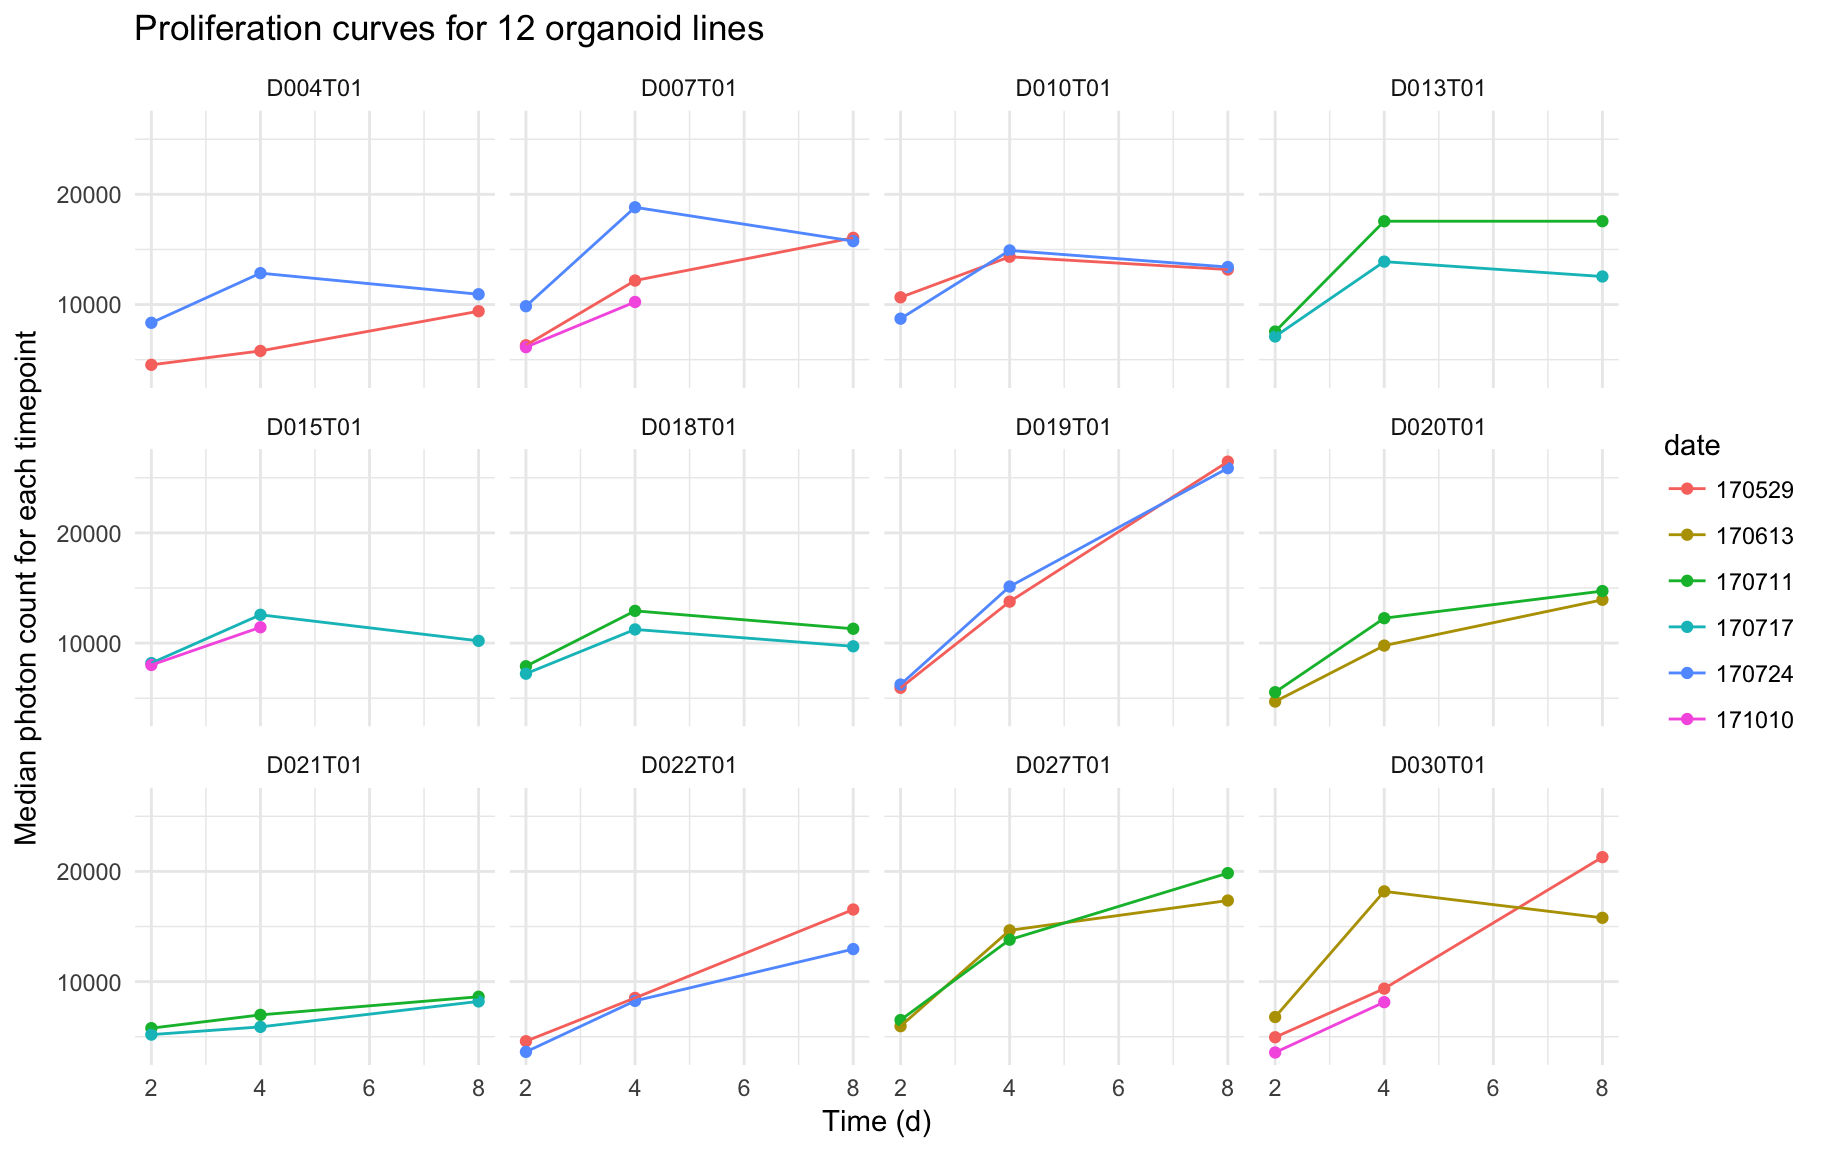
\includegraphics{mofa_exploration_files/figure-latex/unnamed-chunk-25-1.pdf}

\begin{Shaded}
\begin{Highlighting}[]
\NormalTok{df <-}\StringTok{ }\NormalTok{loadings_expression }\OperatorTok\StringTok{ }
\StringTok{  }\KeywordTok{separate}\NormalTok{(id, }\KeywordTok{c}\NormalTok{(}\StringTok{"symbol"}\NormalTok{), }\DataTypeTok{sep =} \StringTok{"_exp"}\NormalTok{) }\OperatorTok\StringTok{ }
\StringTok{  }\KeywordTok{filter}\NormalTok{(symbol }\OperatorTok{!=}\StringTok{ ""}\NormalTok{) }\OperatorTok
\StringTok{  }\KeywordTok{left_join}\NormalTok{(promise_long_filtered_top }\OperatorTok\StringTok{ }\NormalTok{dplyr}\OperatorTok{::}\KeywordTok{select}\NormalTok{(symbol, entrez) }\OperatorTok\StringTok{ }\KeywordTok{distinct}\NormalTok{()) }\OperatorTok
\StringTok{  }\KeywordTok{arrange}\NormalTok{(}\KeywordTok{desc}\NormalTok{(factor1))}
\end{Highlighting}
\end{Shaded}

\begin{verbatim}
## Warning: Expected 1 pieces. Additional pieces discarded in 3222 rows [1, 2, 3,
## 4, 5, 6, 7, 8, 9, 10, 11, 12, 13, 14, 15, 16, 17, 18, 19, 20, ...].
\end{verbatim}

\begin{verbatim}
## Joining, by = "symbol"
\end{verbatim}

\begin{Shaded}
\begin{Highlighting}[]
\NormalTok{ranks_}\DecValTok{1}\NormalTok{ <-}\StringTok{ }\KeywordTok{setNames}\NormalTok{(df}\OperatorTok{$}\NormalTok{factor1, }\KeywordTok{as.character}\NormalTok{(df}\OperatorTok{$}\NormalTok{entrez))}
\NormalTok{ranks_}\DecValTok{1}\NormalTok{ <-}\StringTok{ }\KeywordTok{sort}\NormalTok{(ranks_}\DecValTok{1}\NormalTok{, }\DataTypeTok{decreasing =}\NormalTok{ T)}

\CommentTok{## Reactome enrichment analysis}
\NormalTok{gse_reactome_}\DecValTok{1}\NormalTok{ <-}\StringTok{ }\KeywordTok{gsePathway}\NormalTok{(}
  \DataTypeTok{geneList =}\NormalTok{ ranks_}\DecValTok{1}\NormalTok{,}
  \DataTypeTok{organism =} \StringTok{'human'}\NormalTok{,}
  \CommentTok{#nPerm = 1e5,}
  \CommentTok{#minGSSize = 100,}
  \CommentTok{#maxGSSize = 500,}
  \DataTypeTok{pvalueCutoff =} \FloatTok{0.2}
\NormalTok{)}
\end{Highlighting}
\end{Shaded}

\begin{verbatim}
## Loading required package: org.Hs.eg.db
\end{verbatim}

\begin{verbatim}
## Loading required package: AnnotationDbi
\end{verbatim}

\begin{verbatim}
## Loading required package: stats4
\end{verbatim}

\begin{verbatim}
## Loading required package: BiocGenerics
\end{verbatim}

\begin{verbatim}
## Loading required package: parallel
\end{verbatim}

\begin{verbatim}
## 
## Attaching package: 'BiocGenerics'
\end{verbatim}

\begin{verbatim}
## The following objects are masked from 'package:parallel':
## 
##     clusterApply, clusterApplyLB, clusterCall, clusterEvalQ,
##     clusterExport, clusterMap, parApply, parCapply, parLapply,
##     parLapplyLB, parRapply, parSapply, parSapplyLB
\end{verbatim}

\begin{verbatim}
## The following objects are masked from 'package:dplyr':
## 
##     combine, intersect, setdiff, union
\end{verbatim}

\begin{verbatim}
## The following objects are masked from 'package:stats':
## 
##     IQR, mad, sd, var, xtabs
\end{verbatim}

\begin{verbatim}
## The following objects are masked from 'package:base':
## 
##     anyDuplicated, append, as.data.frame, basename, cbind, colnames,
##     dirname, do.call, duplicated, eval, evalq, Filter, Find, get, grep,
##     grepl, intersect, is.unsorted, lapply, Map, mapply, match, mget,
##     order, paste, pmax, pmax.int, pmin, pmin.int, Position, rank,
##     rbind, Reduce, rownames, sapply, setdiff, sort, table, tapply,
##     union, unique, unsplit, which.max, which.min
\end{verbatim}

\begin{verbatim}
## Loading required package: Biobase
\end{verbatim}

\begin{verbatim}
## Welcome to Bioconductor
## 
##     Vignettes contain introductory material; view with
##     'browseVignettes()'. To cite Bioconductor, see
##     'citation("Biobase")', and for packages 'citation("pkgname")'.
\end{verbatim}

\begin{verbatim}
## Loading required package: IRanges
\end{verbatim}

\begin{verbatim}
## Loading required package: S4Vectors
\end{verbatim}

\begin{verbatim}
## 
## Attaching package: 'S4Vectors'
\end{verbatim}

\begin{verbatim}
## The following object is masked from 'package:clusterProfiler':
## 
##     rename
\end{verbatim}

\begin{verbatim}
## The following objects are masked from 'package:dplyr':
## 
##     first, rename
\end{verbatim}

\begin{verbatim}
## The following object is masked from 'package:tidyr':
## 
##     expand
\end{verbatim}

\begin{verbatim}
## The following object is masked from 'package:base':
## 
##     expand.grid
\end{verbatim}

\begin{verbatim}
## 
## Attaching package: 'IRanges'
\end{verbatim}

\begin{verbatim}
## The following object is masked from 'package:clusterProfiler':
## 
##     slice
\end{verbatim}

\begin{verbatim}
## The following objects are masked from 'package:dplyr':
## 
##     collapse, desc, slice
\end{verbatim}

\begin{verbatim}
## The following object is masked from 'package:purrr':
## 
##     reduce
\end{verbatim}

\begin{verbatim}
## 
## Attaching package: 'AnnotationDbi'
\end{verbatim}

\begin{verbatim}
## The following object is masked from 'package:clusterProfiler':
## 
##     select
\end{verbatim}

\begin{verbatim}
## The following object is masked from 'package:dplyr':
## 
##     select
\end{verbatim}

\begin{verbatim}
## 
\end{verbatim}

\begin{verbatim}
## preparing geneSet collections...
\end{verbatim}

\begin{verbatim}
## GSEA analysis...
\end{verbatim}

\begin{verbatim}
## Warning in preparePathwaysAndStats(pathways, stats, minSize, maxSize,
## gseaParam, : There are duplicate gene names, fgsea may produce unexpected
## results.
\end{verbatim}

\begin{verbatim}
## leading edge analysis...
\end{verbatim}

\begin{verbatim}
## done...
\end{verbatim}

\begin{Shaded}
\begin{Highlighting}[]
\NormalTok{reactome <-}\StringTok{ }\KeywordTok{pairwise_termsim}\NormalTok{(gse_reactome_}\DecValTok{1}\NormalTok{) }
\NormalTok{gg_f1_emap <-}\StringTok{ }\KeywordTok{emapplot}\NormalTok{(reactome, }\DataTypeTok{color =} \StringTok{"NES"}\NormalTok{,}
         \DataTypeTok{cex_label_category =} \FloatTok{.8}\NormalTok{,}
         \DataTypeTok{cex_line =} \DecValTok{1}\NormalTok{) }\OperatorTok{+}\StringTok{ }
\StringTok{  }\KeywordTok{scale_color_viridis_c}\NormalTok{() }\OperatorTok{+}\StringTok{ }
\StringTok{  }\KeywordTok{labs}\NormalTok{(}\DataTypeTok{color =} \StringTok{"NES"}\NormalTok{)}
\end{Highlighting}
\end{Shaded}

\begin{verbatim}
## Scale for 'colour' is already present. Adding another scale for 'colour',
## which will replace the existing scale.
\end{verbatim}

\begin{Shaded}
\begin{Highlighting}[]
\NormalTok{gg_f1_emap }\OperatorTok{+}\StringTok{ }
\StringTok{  }\KeywordTok{ggsave}\NormalTok{(here}\OperatorTok{::}\KeywordTok{here}\NormalTok{(}\StringTok{"reports/figures/mofa/f1_emap.pdf"}\NormalTok{), }\DataTypeTok{width =} \DecValTok{4}\NormalTok{, }\DataTypeTok{height =} \DecValTok{4}\NormalTok{)}
\end{Highlighting}
\end{Shaded}

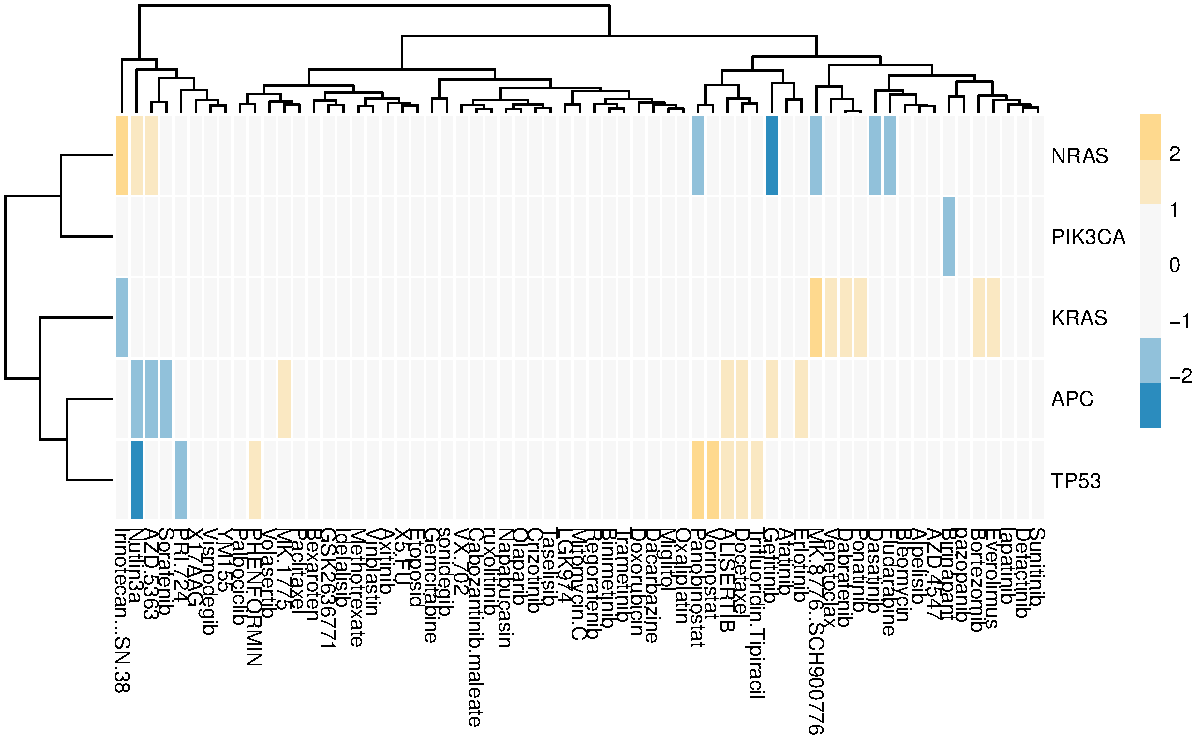
\includegraphics{mofa_exploration_files/figure-latex/unnamed-chunk-26-1.pdf}

\begin{Shaded}
\begin{Highlighting}[]
\NormalTok{gse_go <-}\StringTok{ }\KeywordTok{gseGO}\NormalTok{(}
  \DataTypeTok{geneList =}\NormalTok{ ranks_}\DecValTok{1}\NormalTok{,}
  \DataTypeTok{OrgDb =}\NormalTok{ org.Hs.eg.db,}
  \DataTypeTok{ont =} \StringTok{'BP'}\NormalTok{,}
  \CommentTok{# nPerm = 1e5,}
  \CommentTok{# minGSSize = 10,}
  \CommentTok{# maxGSSize = 500,}
  \DataTypeTok{pvalueCutoff =} \FloatTok{0.2}
\NormalTok{)}

\NormalTok{go <-}\StringTok{ }\KeywordTok{pairwise_termsim}\NormalTok{(gse_go) }
\KeywordTok{emapplot}\NormalTok{(go, }\DataTypeTok{color =} \StringTok{"NES"}\NormalTok{)}
\end{Highlighting}
\end{Shaded}

\hypertarget{suarez-signature}{%
\subsubsection{suarez signature}\label{suarez-signature}}

\begin{Shaded}
\begin{Highlighting}[]
\CommentTok{# run gsea with clusterprofiler}
\NormalTok{df =}\StringTok{ }\NormalTok{loadings_expression }\OperatorTok\StringTok{ }\KeywordTok{drop_na}\NormalTok{() }\OperatorTok
\StringTok{  }\KeywordTok{mutate}\NormalTok{(}\DataTypeTok{symbol =} \KeywordTok{substr}\NormalTok{(id, }\DecValTok{1}\NormalTok{, }\KeywordTok{nchar}\NormalTok{(id)}\OperatorTok{-}\DecValTok{11}\NormalTok{)) }\OperatorTok
\StringTok{  }\NormalTok{dplyr}\OperatorTok{::}\KeywordTok{select}\NormalTok{(}\OperatorTok{-}\NormalTok{id) }\OperatorTok
\StringTok{  }\KeywordTok{left_join}\NormalTok{(promise_long_filtered_top) }\OperatorTok
\StringTok{  }\NormalTok{dplyr}\OperatorTok{::}\KeywordTok{select}\NormalTok{(factor1, symbol) }\OperatorTok\StringTok{ }\KeywordTok{distinct}\NormalTok{() }\OperatorTok
\StringTok{  }\KeywordTok{arrange}\NormalTok{(}\KeywordTok{desc}\NormalTok{(factor1))}
\end{Highlighting}
\end{Shaded}

\begin{verbatim}
## Joining, by = "symbol"
\end{verbatim}

\begin{Shaded}
\begin{Highlighting}[]
\NormalTok{ranks_symbol =}\StringTok{ }\KeywordTok{setNames}\NormalTok{(df}\OperatorTok{$}\NormalTok{factor1, }\KeywordTok{as.character}\NormalTok{(df}\OperatorTok{$}\NormalTok{symbol))}

\NormalTok{gse_sig <-}\StringTok{ }\KeywordTok{GSEA}\NormalTok{(}
  \DataTypeTok{geneList =}\NormalTok{ ranks_symbol,}
  \DataTypeTok{TERM2GENE =}\NormalTok{ intestinal_sig,}
  \DataTypeTok{nPerm =} \FloatTok{1e5}\NormalTok{,}
  \DataTypeTok{minGSSize =} \DecValTok{1}\NormalTok{,}
  \DataTypeTok{maxGSSize =} \DecValTok{1000}\NormalTok{,}
  \DataTypeTok{pvalueCutoff =} \DecValTok{1}
\NormalTok{)}
\end{Highlighting}
\end{Shaded}

\begin{verbatim}
## preparing geneSet collections...
\end{verbatim}

\begin{verbatim}
## GSEA analysis...
\end{verbatim}

\begin{verbatim}
## Warning in .GSEA(geneList = geneList, exponent = exponent, minGSSize =
## minGSSize, : We do not recommend using nPerm parameter incurrent and future
## releases
\end{verbatim}

\begin{verbatim}
## Warning in fgsea(pathways = geneSets, stats = geneList, nperm = nPerm, minSize
## = minGSSize, : You are trying to run fgseaSimple. It is recommended to use
## fgseaMultilevel. To run fgseaMultilevel, you need to remove the nperm argument
## in the fgsea function call.
\end{verbatim}

\begin{verbatim}
## leading edge analysis...
\end{verbatim}

\begin{verbatim}
## done...
\end{verbatim}

\begin{Shaded}
\begin{Highlighting}[]
\CommentTok{## output as tibble}
\NormalTok{gse_sig_tbl <-}\StringTok{ }\KeywordTok{as_tibble}\NormalTok{(gse_sig)}
\end{Highlighting}
\end{Shaded}

\begin{Shaded}
\begin{Highlighting}[]
\CommentTok{## proliferation}
\NormalTok{gg_f1prolif <-}\StringTok{ }\KeywordTok{gseaplot2}\NormalTok{(}
\NormalTok{  gse_sig, }\DataTypeTok{geneSetID =}\NormalTok{ gse_sig}\OperatorTok{$}\NormalTok{ID[}\DecValTok{1}\NormalTok{],}
  \DataTypeTok{title =} \KeywordTok{paste0}\NormalTok{(gse_sig}\OperatorTok{$}\NormalTok{ID[}\DecValTok{1}\NormalTok{], }
                \StringTok{' (p = '}\NormalTok{, }\KeywordTok{round}\NormalTok{(gse_sig_tbl}\OperatorTok{$}\NormalTok{pvalue[}\DecValTok{1}\NormalTok{], }\DecValTok{3}\NormalTok{), }
                \StringTok{'; NES = '}\NormalTok{, }\KeywordTok{round}\NormalTok{(gse_sig_tbl}\OperatorTok{$}\NormalTok{NES[}\DecValTok{1}\NormalTok{], }\DecValTok{2}\NormalTok{), }\StringTok{')'}\NormalTok{)}
\NormalTok{)}

\NormalTok{gg_f1prolif }\OperatorTok{+}\StringTok{ }
\StringTok{  }\KeywordTok{ggsave}\NormalTok{(here}\OperatorTok{::}\KeywordTok{here}\NormalTok{(}\StringTok{"reports/figures/mofa/f1_prolif.pdf"}\NormalTok{), }\DataTypeTok{width =} \DecValTok{4}\NormalTok{, }\DataTypeTok{height =} \DecValTok{3}\NormalTok{)}
\end{Highlighting}
\end{Shaded}

\includegraphics{mofa_exploration_files/figure-latex/unnamed-chunk-29-1.pdf}

\begin{Shaded}
\begin{Highlighting}[]
\CommentTok{## late TA signature}
\KeywordTok{gseaplot2}\NormalTok{(}
\NormalTok{  gse_sig, }\DataTypeTok{geneSetID =}\NormalTok{ gse_sig}\OperatorTok{$}\NormalTok{ID[}\DecValTok{2}\NormalTok{], }
  \DataTypeTok{title =} \KeywordTok{paste0}\NormalTok{(gse_sig}\OperatorTok{$}\NormalTok{ID[}\DecValTok{2}\NormalTok{], }
                \StringTok{' (p = '}\NormalTok{, }\KeywordTok{round}\NormalTok{(gse_sig_tbl}\OperatorTok{$}\NormalTok{pvalue[}\DecValTok{2}\NormalTok{], }\DecValTok{3}\NormalTok{), }
                \StringTok{'; NES = '}\NormalTok{, }\KeywordTok{round}\NormalTok{(gse_sig_tbl}\OperatorTok{$}\NormalTok{NES[}\DecValTok{2}\NormalTok{], }\DecValTok{2}\NormalTok{), }\StringTok{')'}\NormalTok{)}
\NormalTok{) }
\end{Highlighting}
\end{Shaded}

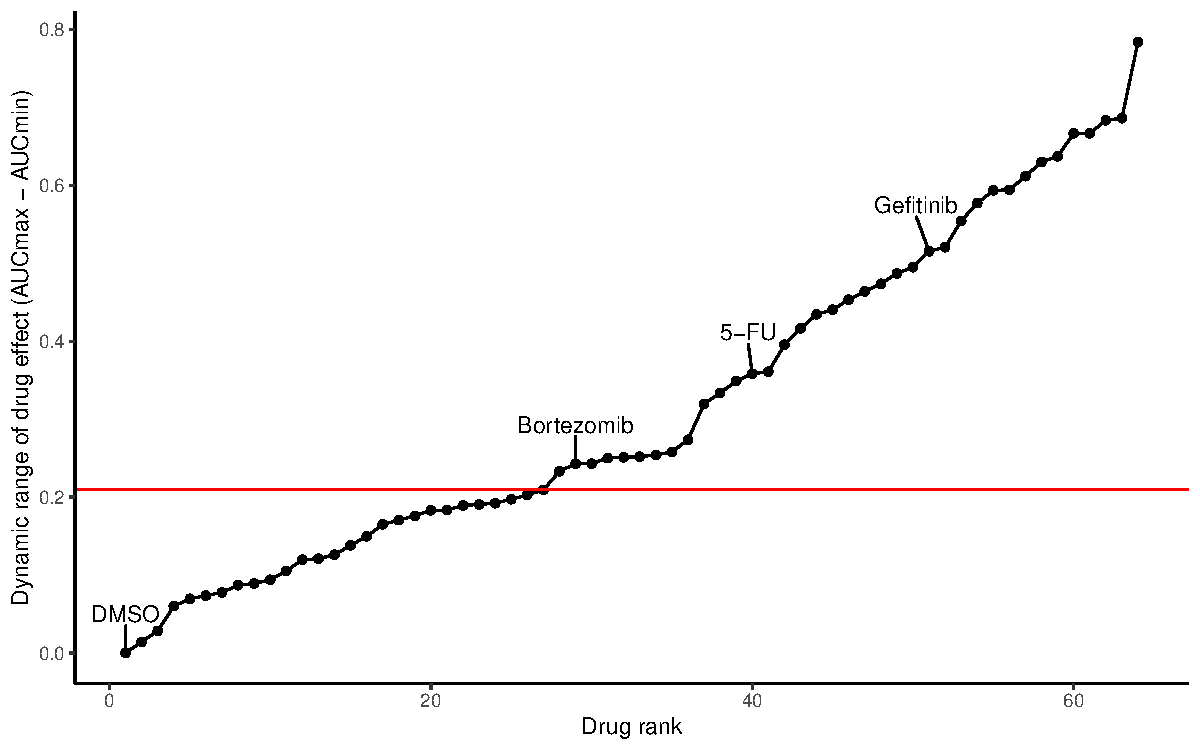
\includegraphics{mofa_exploration_files/figure-latex/unnamed-chunk-30-1.pdf}

\begin{Shaded}
\begin{Highlighting}[]
\CommentTok{## LGR5}
\KeywordTok{gseaplot2}\NormalTok{(}
\NormalTok{  gse_sig, }\DataTypeTok{geneSetID =}\NormalTok{ gse_sig}\OperatorTok{$}\NormalTok{ID[}\DecValTok{3}\NormalTok{],}
  \DataTypeTok{title =} \KeywordTok{paste0}\NormalTok{(gse_sig}\OperatorTok{$}\NormalTok{ID[}\DecValTok{3}\NormalTok{], }
                \StringTok{' (p = '}\NormalTok{, }\KeywordTok{round}\NormalTok{(gse_sig_tbl}\OperatorTok{$}\NormalTok{pvalue[}\DecValTok{3}\NormalTok{], }\DecValTok{3}\NormalTok{), }
                \StringTok{'; NES = '}\NormalTok{, }\KeywordTok{round}\NormalTok{(gse_sig_tbl}\OperatorTok{$}\NormalTok{NES[}\DecValTok{3}\NormalTok{], }\DecValTok{2}\NormalTok{), }\StringTok{')'}\NormalTok{)}
\NormalTok{)}
\end{Highlighting}
\end{Shaded}

\includegraphics{mofa_exploration_files/figure-latex/unnamed-chunk-31-1.pdf}

\begin{Shaded}
\begin{Highlighting}[]
\CommentTok{## EPH}
\KeywordTok{gseaplot2}\NormalTok{(}
\NormalTok{  gse_sig, }\DataTypeTok{geneSetID =}\NormalTok{ gse_sig}\OperatorTok{$}\NormalTok{ID[}\DecValTok{4}\NormalTok{],}
  \DataTypeTok{title =} \KeywordTok{paste0}\NormalTok{(gse_sig}\OperatorTok{$}\NormalTok{ID[}\DecValTok{4}\NormalTok{], }
                \StringTok{' (p = '}\NormalTok{, }\KeywordTok{round}\NormalTok{(gse_sig_tbl}\OperatorTok{$}\NormalTok{pvalue[}\DecValTok{1}\NormalTok{], }\DecValTok{3}\NormalTok{), }
                \StringTok{'; NES = '}\NormalTok{, }\KeywordTok{round}\NormalTok{(gse_sig_tbl}\OperatorTok{$}\NormalTok{NES[}\DecValTok{1}\NormalTok{], }\DecValTok{2}\NormalTok{), }\StringTok{')'}\NormalTok{)}
\NormalTok{)}
\end{Highlighting}
\end{Shaded}

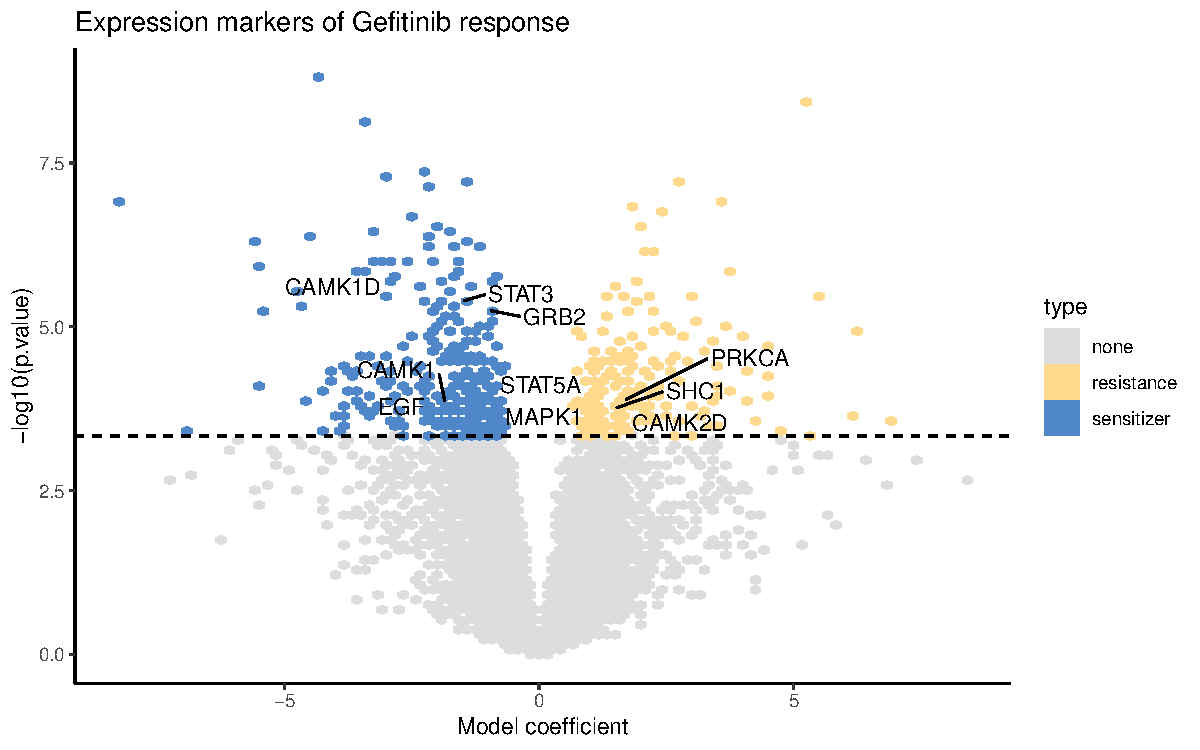
\includegraphics{mofa_exploration_files/figure-latex/unnamed-chunk-32-1.pdf}

\hypertarget{cris-signature}{%
\subsubsection{CRIS signature}\label{cris-signature}}

\begin{Shaded}
\begin{Highlighting}[]
\CommentTok{# run gsea with clusterprofiler}
\NormalTok{df =}\StringTok{ }\NormalTok{loadings_expression }\OperatorTok\StringTok{ }\KeywordTok{drop_na}\NormalTok{() }\OperatorTok
\StringTok{  }\KeywordTok{mutate}\NormalTok{(}\DataTypeTok{symbol =} \KeywordTok{substr}\NormalTok{(id, }\DecValTok{1}\NormalTok{, }\KeywordTok{nchar}\NormalTok{(id)}\OperatorTok{-}\DecValTok{11}\NormalTok{)) }\OperatorTok
\StringTok{  }\NormalTok{dplyr}\OperatorTok{::}\KeywordTok{select}\NormalTok{(}\OperatorTok{-}\NormalTok{id) }\OperatorTok
\StringTok{  }\KeywordTok{left_join}\NormalTok{(promise_long_filtered_top) }\OperatorTok
\StringTok{  }\NormalTok{dplyr}\OperatorTok{::}\KeywordTok{select}\NormalTok{(factor1, symbol) }\OperatorTok\StringTok{ }\KeywordTok{distinct}\NormalTok{() }\OperatorTok
\StringTok{  }\KeywordTok{arrange}\NormalTok{(}\KeywordTok{desc}\NormalTok{(factor1))}
\end{Highlighting}
\end{Shaded}

\begin{verbatim}
## Joining, by = "symbol"
\end{verbatim}

\begin{Shaded}
\begin{Highlighting}[]
\NormalTok{ranks_symbol =}\StringTok{ }\KeywordTok{setNames}\NormalTok{(df}\OperatorTok{$}\NormalTok{factor1, }\KeywordTok{as.character}\NormalTok{(df}\OperatorTok{$}\NormalTok{symbol))}

\NormalTok{gse_cris <-}\StringTok{ }\KeywordTok{GSEA}\NormalTok{(}
  \DataTypeTok{geneList =}\NormalTok{ ranks_symbol,}
  \DataTypeTok{TERM2GENE =}\NormalTok{ cris_sig }\OperatorTok\StringTok{ }\NormalTok{dplyr}\OperatorTok{::}\KeywordTok{select}\NormalTok{(signature, symbol),}
  \DataTypeTok{nPerm =} \FloatTok{1e5}\NormalTok{,}
  \DataTypeTok{minGSSize =} \DecValTok{1}\NormalTok{,}
  \DataTypeTok{maxGSSize =} \DecValTok{1000}\NormalTok{,}
  \DataTypeTok{pvalueCutoff =} \DecValTok{1}
\NormalTok{)}
\end{Highlighting}
\end{Shaded}

\begin{verbatim}
## preparing geneSet collections...
\end{verbatim}

\begin{verbatim}
## GSEA analysis...
\end{verbatim}

\begin{verbatim}
## Warning in .GSEA(geneList = geneList, exponent = exponent, minGSSize =
## minGSSize, : We do not recommend using nPerm parameter incurrent and future
## releases
\end{verbatim}

\begin{verbatim}
## Warning in fgsea(pathways = geneSets, stats = geneList, nperm = nPerm, minSize
## = minGSSize, : You are trying to run fgseaSimple. It is recommended to use
## fgseaMultilevel. To run fgseaMultilevel, you need to remove the nperm argument
## in the fgsea function call.
\end{verbatim}

\begin{verbatim}
## leading edge analysis...
\end{verbatim}

\begin{verbatim}
## done...
\end{verbatim}

\begin{Shaded}
\begin{Highlighting}[]
\CommentTok{## output as tibble}
\NormalTok{gse_cris_tbl <-}\StringTok{ }\KeywordTok{as_tibble}\NormalTok{(gse_cris)}

\NormalTok{gse_cris_tbl}
\end{Highlighting}
\end{Shaded}

\begin{verbatim}
## # A tibble: 5 x 11
##   ID    Description setSize enrichmentScore    NES  pvalue p.adjust qvalues
##   <chr> <chr>         <int>           <dbl>  <dbl>   <dbl>    <dbl> <lgl>  
## 1 CRIS~ CRIS-D           41           0.620  2.17  2.28e-5 0.000114 NA     
## 2 CRIS~ CRIS-C           75          -0.445 -1.69  1.30e-3 0.00326  NA     
## 3 CRIS~ CRIS-A           88          -0.400 -1.56  5.21e-3 0.00868  NA     
## 4 CRIS~ CRIS-E           48          -0.353 -1.23  1.45e-1 0.181    NA     
## 5 CRIS~ CRIS-B           40           0.246  0.856 7.23e-1 0.723    NA     
## # ... with 3 more variables: rank <dbl>, leading_edge <chr>,
## #   core_enrichment <chr>
\end{verbatim}

\begin{Shaded}
\begin{Highlighting}[]
\CommentTok{## proliferation}
\NormalTok{gg_f1_crisc <-}\StringTok{ }\KeywordTok{gseaplot2}\NormalTok{(}
\NormalTok{  gse_cris, }\DataTypeTok{geneSetID =}\NormalTok{ gse_cris}\OperatorTok{$}\NormalTok{ID[}\DecValTok{1}\NormalTok{],}
  \DataTypeTok{title =} \KeywordTok{paste0}\NormalTok{(gse_cris}\OperatorTok{$}\NormalTok{ID[}\DecValTok{1}\NormalTok{], }
                \StringTok{' (p = '}\NormalTok{, }\KeywordTok{round}\NormalTok{(gse_cris_tbl}\OperatorTok{$}\NormalTok{pvalue[}\DecValTok{1}\NormalTok{], }\DecValTok{3}\NormalTok{), }
                \StringTok{'; NES = '}\NormalTok{, }\KeywordTok{round}\NormalTok{(gse_cris_tbl}\OperatorTok{$}\NormalTok{NES[}\DecValTok{1}\NormalTok{], }\DecValTok{2}\NormalTok{), }\StringTok{')'}\NormalTok{)}
\NormalTok{)}

\NormalTok{gg_f1_crisc }\OperatorTok{+}\StringTok{ }
\StringTok{  }\KeywordTok{ggsave}\NormalTok{(here}\OperatorTok{::}\KeywordTok{here}\NormalTok{(}\StringTok{"reports/figures/mofa/f1_crisc.pdf"}\NormalTok{), }\DataTypeTok{width =} \DecValTok{4}\NormalTok{, }\DataTypeTok{height =} \DecValTok{3}\NormalTok{)}
\end{Highlighting}
\end{Shaded}

\includegraphics{mofa_exploration_files/figure-latex/unnamed-chunk-34-1.pdf}

\begin{Shaded}
\begin{Highlighting}[]
\NormalTok{gg_f1_crisd <-}\StringTok{ }\KeywordTok{gseaplot2}\NormalTok{(}
\NormalTok{  gse_cris, }\DataTypeTok{geneSetID =}\NormalTok{ gse_cris}\OperatorTok{$}\NormalTok{ID[}\DecValTok{2}\NormalTok{],}
  \DataTypeTok{title =} \KeywordTok{paste0}\NormalTok{(gse_cris}\OperatorTok{$}\NormalTok{ID[}\DecValTok{2}\NormalTok{], }
                \StringTok{' (p = '}\NormalTok{, }\KeywordTok{round}\NormalTok{(gse_cris_tbl}\OperatorTok{$}\NormalTok{pvalue[}\DecValTok{2}\NormalTok{], }\DecValTok{3}\NormalTok{), }
                \StringTok{'; NES = '}\NormalTok{, }\KeywordTok{round}\NormalTok{(gse_cris_tbl}\OperatorTok{$}\NormalTok{NES[}\DecValTok{2}\NormalTok{], }\DecValTok{2}\NormalTok{), }\StringTok{')'}\NormalTok{)}
\NormalTok{)}

\NormalTok{gg_f1_crisd }\OperatorTok{+}\StringTok{ }
\StringTok{  }\KeywordTok{ggsave}\NormalTok{(here}\OperatorTok{::}\KeywordTok{here}\NormalTok{(}\StringTok{"reports/figures/mofa/f1_crisd.pdf"}\NormalTok{), }\DataTypeTok{width =} \DecValTok{4}\NormalTok{, }\DataTypeTok{height =} \DecValTok{3}\NormalTok{)}
\end{Highlighting}
\end{Shaded}

\includegraphics{mofa_exploration_files/figure-latex/unnamed-chunk-35-1.pdf}

\hypertarget{drug-sensitivity}{%
\subsection{drug sensitivity}\label{drug-sensitivity}}

\begin{Shaded}
\begin{Highlighting}[]
\NormalTok{aggregate_drugs <-}\StringTok{ }\NormalTok{drug_activity_test }\OperatorTok\StringTok{ }\KeywordTok{group_by}\NormalTok{(target) }\OperatorTok\StringTok{ }\KeywordTok{summarise_at}\NormalTok{(}\KeywordTok{vars}\NormalTok{(}\KeywordTok{contains}\NormalTok{(}\StringTok{"factor"}\NormalTok{)), }\KeywordTok{funs}\NormalTok{(}\StringTok{"median"}\NormalTok{))}
\end{Highlighting}
\end{Shaded}

\begin{verbatim}
## Warning: `funs()` is deprecated as of dplyr 0.8.0.
## Please use a list of either functions or lambdas: 
## 
##   # Simple named list: 
##   list(mean = mean, median = median)
## 
##   # Auto named with `tibble::lst()`: 
##   tibble::lst(mean, median)
## 
##   # Using lambdas
##   list(~ mean(., trim = .2), ~ median(., na.rm = TRUE))
## This warning is displayed once every 8 hours.
## Call `lifecycle::last_warnings()` to see where this warning was generated.
\end{verbatim}

\begin{Shaded}
\begin{Highlighting}[]
\NormalTok{include_drugs <-}\StringTok{ }\NormalTok{aggregate_drugs }\OperatorTok\StringTok{ }\KeywordTok{arrange}\NormalTok{(}\KeywordTok{desc}\NormalTok{(factor1)) }\OperatorTok\StringTok{ }\NormalTok{.}\OperatorTok{$}\NormalTok{target}

\NormalTok{gg_f1_drug <-}\StringTok{ }\NormalTok{drug_activity_test }\OperatorTok
\StringTok{  }\KeywordTok{drop_na}\NormalTok{() }\OperatorTok
\StringTok{  }\KeywordTok{mutate}\NormalTok{(}\DataTypeTok{target =} \KeywordTok{factor}\NormalTok{(target, }\DataTypeTok{levels =}\NormalTok{ include_drugs)) }\OperatorTok
\StringTok{  }\KeywordTok{ggplot}\NormalTok{(}\KeywordTok{aes}\NormalTok{(}\DataTypeTok{y =}\NormalTok{ target, }\DataTypeTok{x =}\NormalTok{ factor1)) }\OperatorTok{+}\StringTok{ }
\StringTok{  }\CommentTok{#geom_point() + }
\StringTok{  }\KeywordTok{geom_vline}\NormalTok{(}\DataTypeTok{xintercept =} \DecValTok{0}\NormalTok{, }\DataTypeTok{color =} \StringTok{"grey"}\NormalTok{) }\OperatorTok{+}\StringTok{ }
\StringTok{  }\NormalTok{ggridges}\OperatorTok{::}\KeywordTok{geom_density_ridges}\NormalTok{() }\OperatorTok{+}
\StringTok{  }
\StringTok{  }\CommentTok{#coord_flip() + }
\StringTok{  }\NormalTok{cowplot}\OperatorTok{::}\KeywordTok{theme_cowplot}\NormalTok{()}

\NormalTok{gg_f1_drug }\OperatorTok{+}\StringTok{ }\KeywordTok{ggsave}\NormalTok{(here}\OperatorTok{::}\KeywordTok{here}\NormalTok{(}\StringTok{"reports/figures/mofa/f1_ridge_drug.pdf"}\NormalTok{), }\DataTypeTok{width =} \DecValTok{4}\NormalTok{, }\DataTypeTok{height =} \DecValTok{3}\NormalTok{)}
\end{Highlighting}
\end{Shaded}

\begin{verbatim}
## Picking joint bandwidth of 0.11
## Picking joint bandwidth of 0.11
\end{verbatim}

\includegraphics{mofa_exploration_files/figure-latex/unnamed-chunk-36-1.pdf}

median weighting within the factor was strongest for activity of MEK,
IGF1R inhibitors. mTOR inhibitors ranked among the strongest drugs as
well. In contrast, EGFR inhibitor activity had the most negative median
contribution to the factor. Put differently, organoid lines that had a
high score for factor 1 tended to be sensitive to MEK and IGF-1R
inhibitors and less responsive to EGFR and Syk inhibitors.

EGFR inhibitor activity has a significant negative contribution to the
factor. This means that lines with a high factor1 score, show little to
no activity when treated with EGFR inhibitors.

\begin{Shaded}
\begin{Highlighting}[]
\NormalTok{drug_activity_joined <-}\StringTok{ }\NormalTok{weights }\OperatorTok
\StringTok{  }\KeywordTok{mutate}\NormalTok{(}\DataTypeTok{id =} \KeywordTok{substr}\NormalTok{(id, }\DecValTok{1}\NormalTok{, }\DecValTok{4}\NormalTok{)) }\OperatorTok\StringTok{ }
\StringTok{  }\KeywordTok{group_by}\NormalTok{(id) }\OperatorTok\StringTok{ }
\StringTok{ }\KeywordTok{summarise_all}\NormalTok{(}\KeywordTok{funs}\NormalTok{(mean)) }\OperatorTok\StringTok{ }
\StringTok{  }\KeywordTok{mutate}\NormalTok{(}\DataTypeTok{line =} \KeywordTok{paste0}\NormalTok{(id, }\StringTok{"T01"}\NormalTok{)) }\OperatorTok
\StringTok{  }\KeywordTok{left_join}\NormalTok{(drug_activity)}
\end{Highlighting}
\end{Shaded}

\begin{verbatim}
## Joining, by = "line"
\end{verbatim}

\begin{Shaded}
\begin{Highlighting}[]
\NormalTok{no_egfr <-}\StringTok{ }\KeywordTok{c}\NormalTok{(}\StringTok{"Tyrphostin 9"} \CommentTok{# IC50 at >100uM, binds PDGFR}
\NormalTok{             )}

\NormalTok{doi <-}\StringTok{ }\NormalTok{drug_activity_test }\OperatorTok\StringTok{ }
\StringTok{  }\NormalTok{dplyr}\OperatorTok{::}\KeywordTok{filter}\NormalTok{(target }\OperatorTok{==}\StringTok{ "EGFR"}\NormalTok{) }\OperatorTok\StringTok{ }
\StringTok{  }\NormalTok{dplyr}\OperatorTok{::}\KeywordTok{filter}\NormalTok{(drug }\OperatorTok{!=}\StringTok{ }\NormalTok{no_egfr) }\OperatorTok
\StringTok{  }\NormalTok{.}\OperatorTok{$}\NormalTok{drug }


\NormalTok{gg_f1_egfr <-}\StringTok{ }\NormalTok{drug_activity_joined }\OperatorTok\StringTok{ }
\StringTok{  }\KeywordTok{filter}\NormalTok{(drug }\OperatorTok\StringTok{ }\NormalTok{doi) }\OperatorTok\StringTok{ }
\StringTok{  }\KeywordTok{ggplot}\NormalTok{(}\KeywordTok{aes}\NormalTok{(factor1, auroc)) }\OperatorTok{+}
\StringTok{  }\KeywordTok{geom_point}\NormalTok{() }\OperatorTok{+}\StringTok{ }
\StringTok{  }\NormalTok{cowplot}\OperatorTok{::}\KeywordTok{theme_cowplot}\NormalTok{() }\OperatorTok{+}\StringTok{ }
\StringTok{  }\KeywordTok{geom_smooth}\NormalTok{(}\DataTypeTok{method =} \StringTok{"lm"}\NormalTok{, }\DataTypeTok{se =} \OtherTok{FALSE}\NormalTok{, }\DataTypeTok{color =} \StringTok{"red"}\NormalTok{) }\OperatorTok{+}\StringTok{ }
\StringTok{  }\KeywordTok{facet_wrap}\NormalTok{(}\OperatorTok{~}\StringTok{ }\NormalTok{drug) }\OperatorTok{+}\StringTok{ }
\StringTok{  }\KeywordTok{coord_fixed}\NormalTok{(}\DataTypeTok{ratio =} \DecValTok{5}\NormalTok{)}


\NormalTok{gg_f1_egfr }\OperatorTok{+}\StringTok{ }\KeywordTok{ggsave}\NormalTok{(here}\OperatorTok{::}\KeywordTok{here}\NormalTok{(}\StringTok{"reports/figures/mofa/f1_egfr.pdf"}\NormalTok{), }\DataTypeTok{width =} \DecValTok{6}\NormalTok{, }\DataTypeTok{height =} \DecValTok{6}\NormalTok{)}
\end{Highlighting}
\end{Shaded}

\begin{verbatim}
## `geom_smooth()` using formula 'y ~ x'
\end{verbatim}

\begin{verbatim}
## `geom_smooth()` using formula 'y ~ x'
\end{verbatim}

\includegraphics{mofa_exploration_files/figure-latex/unnamed-chunk-38-1.pdf}

\begin{Shaded}
\begin{Highlighting}[]
\NormalTok{drug_activity_joined <-}\StringTok{ }\NormalTok{weights }\OperatorTok
\StringTok{  }\KeywordTok{mutate}\NormalTok{(}\DataTypeTok{id =} \KeywordTok{substr}\NormalTok{(id, }\DecValTok{1}\NormalTok{, }\DecValTok{4}\NormalTok{)) }\OperatorTok\StringTok{ }
\StringTok{  }\KeywordTok{group_by}\NormalTok{(id) }\OperatorTok\StringTok{ }
\StringTok{ }\KeywordTok{summarise_all}\NormalTok{(}\KeywordTok{funs}\NormalTok{(mean)) }\OperatorTok\StringTok{ }
\StringTok{  }\KeywordTok{mutate}\NormalTok{(}\DataTypeTok{line =} \KeywordTok{paste0}\NormalTok{(id, }\StringTok{"T01"}\NormalTok{)) }\OperatorTok
\StringTok{  }\KeywordTok{left_join}\NormalTok{(drug_activity)}
\end{Highlighting}
\end{Shaded}

\begin{verbatim}
## Joining, by = "line"
\end{verbatim}

\begin{Shaded}
\begin{Highlighting}[]
\NormalTok{doi <-}\StringTok{ }\NormalTok{drug_activity_test }\OperatorTok\StringTok{ }
\StringTok{  }\NormalTok{dplyr}\OperatorTok{::}\KeywordTok{filter}\NormalTok{(target }\OperatorTok{==}\StringTok{ "MEK"}\NormalTok{) }\OperatorTok\StringTok{ }
\StringTok{  }\NormalTok{.}\OperatorTok{$}\NormalTok{drug }


\NormalTok{gg_f1_mek <-}\StringTok{ }\NormalTok{drug_activity_joined }\OperatorTok\StringTok{ }
\StringTok{  }\KeywordTok{filter}\NormalTok{(drug }\OperatorTok\StringTok{ }\NormalTok{doi) }\OperatorTok\StringTok{ }
\StringTok{  }\KeywordTok{ggplot}\NormalTok{(}\KeywordTok{aes}\NormalTok{(factor1, auroc)) }\OperatorTok{+}
\StringTok{  }\KeywordTok{geom_point}\NormalTok{() }\OperatorTok{+}\StringTok{ }
\StringTok{  }\NormalTok{cowplot}\OperatorTok{::}\KeywordTok{theme_cowplot}\NormalTok{() }\OperatorTok{+}\StringTok{ }
\StringTok{  }\KeywordTok{geom_smooth}\NormalTok{(}\DataTypeTok{method =} \StringTok{"lm"}\NormalTok{, }\DataTypeTok{se =} \OtherTok{FALSE}\NormalTok{) }\OperatorTok{+}\StringTok{ }
\StringTok{  }\KeywordTok{facet_wrap}\NormalTok{(}\OperatorTok{~}\StringTok{ }\NormalTok{drug) }\OperatorTok{+}\StringTok{ }
\StringTok{  }\KeywordTok{coord_fixed}\NormalTok{(}\DataTypeTok{ratio =} \DecValTok{5}\NormalTok{)}

\NormalTok{gg_f1_mek }\OperatorTok{+}\StringTok{ }\KeywordTok{ggsave}\NormalTok{(here}\OperatorTok{::}\KeywordTok{here}\NormalTok{(}\StringTok{"reports/figures/mofa/f1_mek.pdf"}\NormalTok{), }\DataTypeTok{width =} \DecValTok{6}\NormalTok{, }\DataTypeTok{height =} \DecValTok{6}\NormalTok{)}
\end{Highlighting}
\end{Shaded}

\begin{verbatim}
## `geom_smooth()` using formula 'y ~ x'
\end{verbatim}

\begin{verbatim}
## Warning: Removed 1 rows containing non-finite values (stat_smooth).
\end{verbatim}

\begin{verbatim}
## Warning: Removed 1 rows containing missing values (geom_point).
\end{verbatim}

\begin{verbatim}
## `geom_smooth()` using formula 'y ~ x'
\end{verbatim}

\begin{verbatim}
## Warning: Removed 1 rows containing non-finite values (stat_smooth).

## Warning: Removed 1 rows containing missing values (geom_point).
\end{verbatim}

\includegraphics{mofa_exploration_files/figure-latex/unnamed-chunk-39-1.pdf}

\begin{Shaded}
\begin{Highlighting}[]
\NormalTok{drug_activity_joined <-}\StringTok{ }\NormalTok{weights }\OperatorTok
\StringTok{  }\KeywordTok{mutate}\NormalTok{(}\DataTypeTok{id =} \KeywordTok{substr}\NormalTok{(id, }\DecValTok{1}\NormalTok{, }\DecValTok{4}\NormalTok{)) }\OperatorTok\StringTok{ }
\StringTok{  }\KeywordTok{group_by}\NormalTok{(id) }\OperatorTok\StringTok{ }
\StringTok{ }\KeywordTok{summarise_all}\NormalTok{(}\KeywordTok{funs}\NormalTok{(mean)) }\OperatorTok\StringTok{ }
\StringTok{  }\KeywordTok{mutate}\NormalTok{(}\DataTypeTok{line =} \KeywordTok{paste0}\NormalTok{(id, }\StringTok{"T01"}\NormalTok{)) }\OperatorTok
\StringTok{  }\KeywordTok{left_join}\NormalTok{(drug_activity)}
\end{Highlighting}
\end{Shaded}

\begin{verbatim}
## Joining, by = "line"
\end{verbatim}

\begin{Shaded}
\begin{Highlighting}[]
\NormalTok{doi <-}\StringTok{ }\NormalTok{drug_activity_test }\OperatorTok\StringTok{ }
\StringTok{  }\NormalTok{dplyr}\OperatorTok{::}\KeywordTok{filter}\NormalTok{(target }\OperatorTok{==}\StringTok{ "IGF-1R"}\NormalTok{) }\OperatorTok\StringTok{ }
\StringTok{  }\NormalTok{.}\OperatorTok{$}\NormalTok{drug }


\NormalTok{gg_f1_igf <-}\StringTok{ }\NormalTok{drug_activity_joined }\OperatorTok\StringTok{ }
\StringTok{  }\KeywordTok{filter}\NormalTok{(drug }\OperatorTok\StringTok{ }\NormalTok{doi) }\OperatorTok\StringTok{ }
\StringTok{  }\KeywordTok{ggplot}\NormalTok{(}\KeywordTok{aes}\NormalTok{(factor1, auroc)) }\OperatorTok{+}
\StringTok{  }\KeywordTok{geom_point}\NormalTok{() }\OperatorTok{+}\StringTok{ }
\StringTok{  }\NormalTok{cowplot}\OperatorTok{::}\KeywordTok{theme_cowplot}\NormalTok{() }\OperatorTok{+}\StringTok{ }
\StringTok{  }\KeywordTok{geom_smooth}\NormalTok{(}\DataTypeTok{method =} \StringTok{"lm"}\NormalTok{, }\DataTypeTok{se =} \OtherTok{FALSE}\NormalTok{, }\DataTypeTok{color =} \StringTok{"black"}\NormalTok{) }\OperatorTok{+}\StringTok{ }
\StringTok{  }\KeywordTok{facet_wrap}\NormalTok{(}\OperatorTok{~}\StringTok{ }\NormalTok{drug)}

\NormalTok{gg_f1_igf }\OperatorTok{+}\StringTok{ }\KeywordTok{ggsave}\NormalTok{(here}\OperatorTok{::}\KeywordTok{here}\NormalTok{(}\StringTok{"reports/figures/mofa/f1_igf.pdf"}\NormalTok{), }\DataTypeTok{width =} \DecValTok{6}\NormalTok{, }\DataTypeTok{height =} \DecValTok{6}\NormalTok{)}
\end{Highlighting}
\end{Shaded}

\begin{verbatim}
## `geom_smooth()` using formula 'y ~ x'
\end{verbatim}

\begin{verbatim}
## `geom_smooth()` using formula 'y ~ x'
\end{verbatim}

\includegraphics{mofa_exploration_files/figure-latex/unnamed-chunk-40-1.pdf}

\begin{Shaded}
\begin{Highlighting}[]
\NormalTok{drug_activity_joined <-}\StringTok{ }\NormalTok{weights }\OperatorTok
\StringTok{  }\KeywordTok{mutate}\NormalTok{(}\DataTypeTok{id =} \KeywordTok{substr}\NormalTok{(id, }\DecValTok{1}\NormalTok{, }\DecValTok{4}\NormalTok{)) }\OperatorTok\StringTok{ }
\StringTok{  }\KeywordTok{group_by}\NormalTok{(id) }\OperatorTok\StringTok{ }
\StringTok{ }\KeywordTok{summarise_all}\NormalTok{(}\KeywordTok{funs}\NormalTok{(mean)) }\OperatorTok\StringTok{ }
\StringTok{  }\KeywordTok{mutate}\NormalTok{(}\DataTypeTok{line =} \KeywordTok{paste0}\NormalTok{(id, }\StringTok{"T01"}\NormalTok{)) }\OperatorTok
\StringTok{  }\KeywordTok{left_join}\NormalTok{(drug_activity)}
\end{Highlighting}
\end{Shaded}

\begin{verbatim}
## Joining, by = "line"
\end{verbatim}

\begin{Shaded}
\begin{Highlighting}[]
\NormalTok{doi <-}\StringTok{ }\NormalTok{drug_activity_test }\OperatorTok\StringTok{ }
\StringTok{  }\NormalTok{dplyr}\OperatorTok{::}\KeywordTok{filter}\NormalTok{(target }\OperatorTok{==}\StringTok{ "mTOR"}\NormalTok{) }\OperatorTok\StringTok{ }
\StringTok{  }\NormalTok{.}\OperatorTok{$}\NormalTok{drug }


\NormalTok{gg_f1_mtor <-}\StringTok{ }\NormalTok{drug_activity_joined }\OperatorTok\StringTok{ }
\StringTok{  }\KeywordTok{filter}\NormalTok{(drug }\OperatorTok\StringTok{ }\NormalTok{doi) }\OperatorTok\StringTok{ }
\StringTok{  }\KeywordTok{ggplot}\NormalTok{(}\KeywordTok{aes}\NormalTok{(factor1, auroc)) }\OperatorTok{+}
\StringTok{  }\KeywordTok{geom_point}\NormalTok{() }\OperatorTok{+}\StringTok{ }
\StringTok{  }\NormalTok{cowplot}\OperatorTok{::}\KeywordTok{theme_cowplot}\NormalTok{() }\OperatorTok{+}\StringTok{ }
\StringTok{  }\KeywordTok{geom_smooth}\NormalTok{(}\DataTypeTok{method =} \StringTok{"lm"}\NormalTok{, }\DataTypeTok{se =} \OtherTok{FALSE}\NormalTok{, }\DataTypeTok{color =} \StringTok{"green"}\NormalTok{) }\OperatorTok{+}\StringTok{ }
\StringTok{  }\KeywordTok{facet_wrap}\NormalTok{(}\OperatorTok{~}\StringTok{ }\NormalTok{drug)}

\NormalTok{gg_f1_mtor }\OperatorTok{+}\StringTok{ }\KeywordTok{ggsave}\NormalTok{(here}\OperatorTok{::}\KeywordTok{here}\NormalTok{(}\StringTok{"reports/figures/mofa/f1_mtor.pdf"}\NormalTok{), }\DataTypeTok{width =} \DecValTok{6}\NormalTok{, }\DataTypeTok{height =} \DecValTok{6}\NormalTok{)}
\end{Highlighting}
\end{Shaded}

\begin{verbatim}
## `geom_smooth()` using formula 'y ~ x'
\end{verbatim}

\begin{verbatim}
## `geom_smooth()` using formula 'y ~ x'
\end{verbatim}

\includegraphics{mofa_exploration_files/figure-latex/unnamed-chunk-41-1.pdf}
within the group of mTOR inhibitors, activity towards treatment with the
small molecule WYE-132 had the strongest contribution to the factor.
WYE-132 is an ATP competitive inhibitor of mTORC1 and mTORC2

\hypertarget{pick-of-drug-sensitivity}{%
\subsubsection{pick of drug
sensitivity}\label{pick-of-drug-sensitivity}}

\begin{Shaded}
\begin{Highlighting}[]
\NormalTok{gg_f1_egfr_pick <-}\StringTok{ }\NormalTok{drug_activity_joined }\OperatorTok\StringTok{ }
\StringTok{  }\KeywordTok{filter}\NormalTok{(drug }\OperatorTok\StringTok{ }\KeywordTok{c}\NormalTok{(}\StringTok{"OSI-420"}\NormalTok{, }\StringTok{"Trametinib (GSK1120212)"}\NormalTok{, }\StringTok{"BMS-536924"}\NormalTok{)) }\OperatorTok\StringTok{ }
\StringTok{  }\KeywordTok{ggplot}\NormalTok{(}\KeywordTok{aes}\NormalTok{(factor1, auroc, }\DataTypeTok{color =}\NormalTok{ drug)) }\OperatorTok{+}
\StringTok{  }\KeywordTok{geom_point}\NormalTok{() }\OperatorTok{+}\StringTok{ }
\StringTok{  }\NormalTok{cowplot}\OperatorTok{::}\KeywordTok{theme_cowplot}\NormalTok{() }\OperatorTok{+}\StringTok{ }
\StringTok{  }\KeywordTok{geom_smooth}\NormalTok{(}\DataTypeTok{method =} \StringTok{"lm"}\NormalTok{, }\DataTypeTok{se =} \OtherTok{FALSE}\NormalTok{, }\KeywordTok{aes}\NormalTok{(}\DataTypeTok{group =}\NormalTok{ drug)) }\OperatorTok{+}\StringTok{ }
\StringTok{  }\KeywordTok{coord_equal}\NormalTok{(}\DataTypeTok{ratio =} \DecValTok{10}\NormalTok{) }\OperatorTok{+}\StringTok{ }
\StringTok{  }\KeywordTok{theme}\NormalTok{(}\DataTypeTok{legend.position =} \StringTok{"bottom"}\NormalTok{)}
  

\NormalTok{gg_f1_egfr_pick }\OperatorTok{+}\StringTok{ }\KeywordTok{ggsave}\NormalTok{(here}\OperatorTok{::}\KeywordTok{here}\NormalTok{(}\StringTok{"reports/figures/mofa/f1_drug_pick.pdf"}\NormalTok{), }\DataTypeTok{width =} \DecValTok{4}\NormalTok{, }\DataTypeTok{height =} \DecValTok{4}\NormalTok{)}
\end{Highlighting}
\end{Shaded}

\begin{verbatim}
## `geom_smooth()` using formula 'y ~ x'
## `geom_smooth()` using formula 'y ~ x'
\end{verbatim}

\includegraphics{mofa_exploration_files/figure-latex/unnamed-chunk-42-1.pdf}

Next we wondered how treatment with members from these highly active
groups would change the phenotype of organoids

\hypertarget{mutation}{%
\subsection{mutation}\label{mutation}}

\begin{Shaded}
\begin{Highlighting}[]
\NormalTok{df <-}\StringTok{ }\NormalTok{mofa_genetics }\OperatorTok\StringTok{ }
\StringTok{  }\KeywordTok{mutate}\NormalTok{(}\DataTypeTok{sample =} \KeywordTok{substr}\NormalTok{(sample, }\DecValTok{1}\NormalTok{, }\DecValTok{4}\NormalTok{)) }\OperatorTok\StringTok{ }
\StringTok{  }\KeywordTok{distinct}\NormalTok{() }\OperatorTok
\StringTok{  }\KeywordTok{filter}\NormalTok{(feature }\OperatorTok\StringTok{ }\KeywordTok{c}\NormalTok{(}\StringTok{"NRAS"}\NormalTok{))}

\NormalTok{drug_activity_joined }\OperatorTok
\StringTok{  }\NormalTok{dplyr}\OperatorTok{::}\KeywordTok{select}\NormalTok{(}\OperatorTok{-}\NormalTok{line, }\DataTypeTok{sample =}\NormalTok{ id) }\OperatorTok\StringTok{ }
\StringTok{  }\KeywordTok{filter}\NormalTok{(drug }\OperatorTok\StringTok{ }\KeywordTok{c}\NormalTok{(}\StringTok{"Selumetinib (AZD6244)"}\NormalTok{)) }\OperatorTok
\StringTok{  }\KeywordTok{left_join}\NormalTok{(df) }\OperatorTok\StringTok{ }
\StringTok{  }\KeywordTok{drop_na}\NormalTok{() }\OperatorTok
\StringTok{  }\KeywordTok{mutate}\NormalTok{(}\DataTypeTok{value =} \KeywordTok{if_else}\NormalTok{(value }\OperatorTok{==}\StringTok{ }\DecValTok{0}\NormalTok{, }\StringTok{"WT"}\NormalTok{, }\StringTok{"mut"}\NormalTok{)) }\OperatorTok
\StringTok{  }\KeywordTok{ggplot}\NormalTok{(}\KeywordTok{aes}\NormalTok{(value, auroc)) }\OperatorTok{+}\StringTok{ }
\StringTok{  }\KeywordTok{geom_point}\NormalTok{() }\OperatorTok{+}\StringTok{ }
\StringTok{  }\NormalTok{ggsignif}\OperatorTok{::}\KeywordTok{geom_signif}\NormalTok{(}\DataTypeTok{comparisons =} \KeywordTok{list}\NormalTok{(}\KeywordTok{c}\NormalTok{(}\StringTok{"WT"}\NormalTok{, }\StringTok{"mut"}\NormalTok{))) }\OperatorTok{+}\StringTok{ }
\StringTok{  }\KeywordTok{theme_cowplot}\NormalTok{() }\OperatorTok{+}\StringTok{ }
\StringTok{  }\KeywordTok{facet_grid}\NormalTok{(drug }\OperatorTok{~}\StringTok{ }\NormalTok{feature)}
\end{Highlighting}
\end{Shaded}

\begin{verbatim}
## Joining, by = "sample"
\end{verbatim}

\includegraphics{mofa_exploration_files/figure-latex/unnamed-chunk-43-1.pdf}

\hypertarget{panel}{%
\subsection{panel}\label{panel}}

\begin{Shaded}
\begin{Highlighting}[]
\KeywordTok{plot_grid}\NormalTok{(}\KeywordTok{plot_grid}\NormalTok{(gg_sizef1, gg_f1_geneexp, }\DataTypeTok{align =} \StringTok{"hv"}\NormalTok{), }
\NormalTok{          gg_f1_emap,}
          \KeywordTok{plot_grid}\NormalTok{(gg_f1prolif, gg_f1_crisc, gg_f1_crisd, }\DataTypeTok{ncol =} \DecValTok{1}\NormalTok{),}
\NormalTok{          gg_f1_drug}
\NormalTok{          )}
\end{Highlighting}
\end{Shaded}

\hypertarget{factor-2}{%
\section{factor 2}\label{factor-2}}

\hypertarget{morphology}{%
\subsection{morphology}\label{morphology}}

\begin{Shaded}
\begin{Highlighting}[]
\NormalTok{gg_cystic <-}\StringTok{ }\NormalTok{weights }\OperatorTok\StringTok{ }
\StringTok{  }\NormalTok{dplyr}\OperatorTok{::}\KeywordTok{rename}\NormalTok{(}\DataTypeTok{line =}\NormalTok{ id) }\OperatorTok
\StringTok{  }\KeywordTok{left_join}\NormalTok{(organoid_morphology }\OperatorTok\StringTok{ }
\StringTok{              }\KeywordTok{mutate}\NormalTok{(}\DataTypeTok{line =} \KeywordTok{substr}\NormalTok{(line, }\DecValTok{1}\NormalTok{, }\DecValTok{4}\NormalTok{)) }\OperatorTok\StringTok{ }
\StringTok{    }\KeywordTok{expand_grid}\NormalTok{(., }\DataTypeTok{rep =} \KeywordTok{c}\NormalTok{(}\StringTok{"r1"}\NormalTok{, }\StringTok{"r2"}\NormalTok{)) }\OperatorTok\StringTok{ }
\StringTok{      }\KeywordTok{mutate}\NormalTok{(}\DataTypeTok{sample =} \KeywordTok{paste0}\NormalTok{(line, }\StringTok{"_"}\NormalTok{, rep)) }\OperatorTok\StringTok{ }\NormalTok{dplyr}\OperatorTok{::}\KeywordTok{select}\NormalTok{(}\OperatorTok{-}\NormalTok{line, }\DataTypeTok{line =}\NormalTok{ sample)) }\OperatorTok
\StringTok{  }\KeywordTok{distinct}\NormalTok{() }\OperatorTok
\StringTok{  }\KeywordTok{ggplot}\NormalTok{(}\KeywordTok{aes}\NormalTok{(factor1, factor2, }\DataTypeTok{label =}\NormalTok{ line, }\DataTypeTok{color =}\NormalTok{ morphology)) }\OperatorTok{+}\StringTok{ }
\StringTok{  }\KeywordTok{geom_point}\NormalTok{(}\DataTypeTok{size =} \DecValTok{4}\NormalTok{) }\OperatorTok{+}\StringTok{ }
\StringTok{  }\NormalTok{ggrepel}\OperatorTok{::}\KeywordTok{geom_text_repel}\NormalTok{(}\DataTypeTok{color =} \StringTok{"black"}\NormalTok{) }\OperatorTok{+}\StringTok{ }
\StringTok{  }\KeywordTok{theme_cowplot}\NormalTok{() }\OperatorTok{+}\StringTok{ }
\StringTok{  }\KeywordTok{scale_color_brewer}\NormalTok{(}\DataTypeTok{type =} \StringTok{"qual"}\NormalTok{)}
\end{Highlighting}
\end{Shaded}

\begin{verbatim}
## Joining, by = "line"
\end{verbatim}

\begin{Shaded}
\begin{Highlighting}[]
\NormalTok{gg_cystic }\OperatorTok{+}\StringTok{ }\KeywordTok{ggsave}\NormalTok{(here}\OperatorTok{::}\KeywordTok{here}\NormalTok{(}\StringTok{"reports/figures/mofa/f2_morph.pdf"}\NormalTok{), }\DataTypeTok{width =} \DecValTok{6}\NormalTok{, }\DataTypeTok{height =} \DecValTok{6}\NormalTok{)}
\end{Highlighting}
\end{Shaded}

\includegraphics{mofa_exploration_files/figure-latex/unnamed-chunk-45-1.pdf}

\hypertarget{gene-expression-1}{%
\subsection{gene expression}\label{gene-expression-1}}

\begin{Shaded}
\begin{Highlighting}[]
\NormalTok{gg_f2_geneexp <-}\StringTok{ }\KeywordTok{plot_weights}\NormalTok{(model,}
  \DataTypeTok{view =} \StringTok{"expression"}\NormalTok{,}
  \DataTypeTok{factor =} \DecValTok{2}\NormalTok{,}
  \DataTypeTok{nfeatures =} \DecValTok{10}\NormalTok{,     }\CommentTok{# Number of features to highlight}
  \DataTypeTok{scale =}\NormalTok{ T,          }\CommentTok{# Scale weights from -1 to 1}
  \DataTypeTok{abs =}\NormalTok{ F             }\CommentTok{# Take the absolute value?}
\NormalTok{) }\OperatorTok{+}\StringTok{ }
\StringTok{  }\KeywordTok{theme_cowplot}\NormalTok{() }\OperatorTok{+}\StringTok{ }
\StringTok{  }\KeywordTok{theme}\NormalTok{(}\DataTypeTok{axis.text.y =} \KeywordTok{element_blank}\NormalTok{(),}
        \DataTypeTok{axis.ticks.y =}\KeywordTok{element_blank}\NormalTok{()) }
\end{Highlighting}
\end{Shaded}

\begin{verbatim}
## Warning: Ignoring unknown parameters: max.overlaps
\end{verbatim}

\begin{Shaded}
\begin{Highlighting}[]
\NormalTok{gg_f2_geneexp }\OperatorTok{+}\StringTok{ }
\StringTok{  }\KeywordTok{ggsave}\NormalTok{(here}\OperatorTok{::}\KeywordTok{here}\NormalTok{(}\StringTok{"reports/figures/mofa/f2_genexp.pdf"}\NormalTok{), }\DataTypeTok{width =} \DecValTok{4}\NormalTok{, }\DataTypeTok{height =} \DecValTok{4}\NormalTok{)}
\end{Highlighting}
\end{Shaded}

\includegraphics{mofa_exploration_files/figure-latex/unnamed-chunk-46-1.pdf}
growth control via IGF signaling cell adhesion via FYN signaling, high
fibronectin expression DLX- TGFb and BMP inhibiting transcription factor

\hypertarget{reactome-and-go}{%
\subsubsection{reactome and GO}\label{reactome-and-go}}

\begin{Shaded}
\begin{Highlighting}[]
\NormalTok{df <-}\StringTok{ }\NormalTok{loadings_expression }\OperatorTok\StringTok{ }
\StringTok{  }\KeywordTok{separate}\NormalTok{(id, }\KeywordTok{c}\NormalTok{(}\StringTok{"symbol"}\NormalTok{), }\DataTypeTok{sep =} \StringTok{"_exp"}\NormalTok{) }\OperatorTok\StringTok{ }
\StringTok{  }\KeywordTok{filter}\NormalTok{(symbol }\OperatorTok{!=}\StringTok{ ""}\NormalTok{) }\OperatorTok
\StringTok{  }\KeywordTok{left_join}\NormalTok{(promise_long_filtered_top }\OperatorTok\StringTok{ }\NormalTok{dplyr}\OperatorTok{::}\KeywordTok{select}\NormalTok{(symbol, entrez) }\OperatorTok\StringTok{ }\KeywordTok{distinct}\NormalTok{()) }\OperatorTok
\StringTok{  }\KeywordTok{arrange}\NormalTok{(}\KeywordTok{desc}\NormalTok{(factor2))}
\end{Highlighting}
\end{Shaded}

\begin{verbatim}
## Warning: Expected 1 pieces. Additional pieces discarded in 3222 rows [1, 2, 3,
## 4, 5, 6, 7, 8, 9, 10, 11, 12, 13, 14, 15, 16, 17, 18, 19, 20, ...].
\end{verbatim}

\begin{verbatim}
## Joining, by = "symbol"
\end{verbatim}

\begin{Shaded}
\begin{Highlighting}[]
\NormalTok{ranks_}\DecValTok{2}\NormalTok{ <-}\StringTok{ }\KeywordTok{setNames}\NormalTok{(df}\OperatorTok{$}\NormalTok{factor2, }\KeywordTok{as.character}\NormalTok{(df}\OperatorTok{$}\NormalTok{entrez))}
\NormalTok{ranks_}\DecValTok{2}\NormalTok{ <-}\StringTok{ }\KeywordTok{sort}\NormalTok{(ranks_}\DecValTok{2}\NormalTok{, }\DataTypeTok{decreasing =}\NormalTok{ T)}

\CommentTok{## Reactome enrichment analysis}
\NormalTok{gse_reactome_}\DecValTok{2}\NormalTok{ <-}\StringTok{ }\KeywordTok{gsePathway}\NormalTok{(}
  \DataTypeTok{geneList =}\NormalTok{ ranks_}\DecValTok{2}\NormalTok{,}
  \DataTypeTok{organism =} \StringTok{'human'}\NormalTok{,}
  \CommentTok{#nPerm = 1e5,}
  \CommentTok{#minGSSize = 100,}
  \CommentTok{#maxGSSize = 500,}
  \DataTypeTok{pvalueCutoff =} \FloatTok{0.2}
\NormalTok{)}
\end{Highlighting}
\end{Shaded}

\begin{verbatim}
## preparing geneSet collections...
\end{verbatim}

\begin{verbatim}
## GSEA analysis...
\end{verbatim}

\begin{verbatim}
## Warning in preparePathwaysAndStats(pathways, stats, minSize, maxSize,
## gseaParam, : There are duplicate gene names, fgsea may produce unexpected
## results.
\end{verbatim}

\begin{verbatim}
## leading edge analysis...
\end{verbatim}

\begin{verbatim}
## done...
\end{verbatim}

\begin{Shaded}
\begin{Highlighting}[]
\NormalTok{reactome <-}\StringTok{ }\KeywordTok{pairwise_termsim}\NormalTok{(gse_reactome_}\DecValTok{2}\NormalTok{) }

\NormalTok{gg_f2_emap <-}\StringTok{ }\KeywordTok{emapplot}\NormalTok{(reactome, }\DataTypeTok{color =} \StringTok{"NES"}\NormalTok{,}
         \DataTypeTok{cex_label_category =} \FloatTok{.8}\NormalTok{,}
         \DataTypeTok{cex_line =} \DecValTok{1}\NormalTok{) }\OperatorTok{+}\StringTok{ }
\StringTok{  }\KeywordTok{scale_color_viridis_c}\NormalTok{() }\OperatorTok{+}\StringTok{ }
\StringTok{  }\KeywordTok{labs}\NormalTok{(}\DataTypeTok{color =} \StringTok{"NES"}\NormalTok{)}
\end{Highlighting}
\end{Shaded}

\begin{verbatim}
## Scale for 'colour' is already present. Adding another scale for 'colour',
## which will replace the existing scale.
\end{verbatim}

\begin{Shaded}
\begin{Highlighting}[]
\NormalTok{gg_f2_emap }\OperatorTok{+}\StringTok{ }
\StringTok{  }\KeywordTok{ggsave}\NormalTok{(here}\OperatorTok{::}\KeywordTok{here}\NormalTok{(}\StringTok{"reports/figures/mofa/f2_emap.pdf"}\NormalTok{), }\DataTypeTok{width =} \DecValTok{4}\NormalTok{, }\DataTypeTok{height =} \DecValTok{4}\NormalTok{)}
\end{Highlighting}
\end{Shaded}

\includegraphics{mofa_exploration_files/figure-latex/unnamed-chunk-47-1.pdf}

\begin{Shaded}
\begin{Highlighting}[]
\NormalTok{gse_go <-}\StringTok{ }\KeywordTok{gseGO}\NormalTok{(}
  \DataTypeTok{geneList =}\NormalTok{ ranks_}\DecValTok{2}\NormalTok{,}
  \DataTypeTok{OrgDb =}\NormalTok{ org.Hs.eg.db,}
  \DataTypeTok{ont =} \StringTok{'BP'}\NormalTok{,}
  \CommentTok{# nPerm = 1e5,}
  \CommentTok{# minGSSize = 10,}
  \CommentTok{# maxGSSize = 500,}
  \DataTypeTok{pvalueCutoff =} \FloatTok{0.2}
\NormalTok{)}

\NormalTok{go <-}\StringTok{ }\KeywordTok{pairwise_termsim}\NormalTok{(gse_go) }
\KeywordTok{emapplot}\NormalTok{(go, }\DataTypeTok{color =} \StringTok{"NES"}\NormalTok{)}
\end{Highlighting}
\end{Shaded}

\hypertarget{suarez-signature-1}{%
\subsubsection{suarez signature}\label{suarez-signature-1}}

\begin{Shaded}
\begin{Highlighting}[]
\CommentTok{# run gsea with clusterprofiler}
\NormalTok{df =}\StringTok{ }\NormalTok{loadings_expression }\OperatorTok\StringTok{ }\KeywordTok{drop_na}\NormalTok{() }\OperatorTok
\StringTok{  }\KeywordTok{mutate}\NormalTok{(}\DataTypeTok{symbol =} \KeywordTok{substr}\NormalTok{(id, }\DecValTok{1}\NormalTok{, }\KeywordTok{nchar}\NormalTok{(id)}\OperatorTok{-}\DecValTok{11}\NormalTok{)) }\OperatorTok
\StringTok{  }\NormalTok{dplyr}\OperatorTok{::}\KeywordTok{select}\NormalTok{(}\OperatorTok{-}\NormalTok{id) }\OperatorTok
\StringTok{  }\KeywordTok{left_join}\NormalTok{(promise_long_filtered_top) }\OperatorTok
\StringTok{  }\NormalTok{dplyr}\OperatorTok{::}\KeywordTok{select}\NormalTok{(factor2, symbol) }\OperatorTok\StringTok{ }\KeywordTok{distinct}\NormalTok{() }\OperatorTok
\StringTok{  }\KeywordTok{arrange}\NormalTok{(}\KeywordTok{desc}\NormalTok{(factor2))}
\end{Highlighting}
\end{Shaded}

\begin{verbatim}
## Joining, by = "symbol"
\end{verbatim}

\begin{Shaded}
\begin{Highlighting}[]
\NormalTok{ranks_symbol =}\StringTok{ }\KeywordTok{setNames}\NormalTok{(df}\OperatorTok{$}\NormalTok{factor2, }\KeywordTok{as.character}\NormalTok{(df}\OperatorTok{$}\NormalTok{symbol))}

\NormalTok{gse_sig <-}\StringTok{ }\KeywordTok{GSEA}\NormalTok{(}
  \DataTypeTok{geneList =}\NormalTok{ ranks_symbol,}
  \DataTypeTok{TERM2GENE =}\NormalTok{ intestinal_sig,}
  \DataTypeTok{nPerm =} \FloatTok{1e5}\NormalTok{,}
  \DataTypeTok{minGSSize =} \DecValTok{1}\NormalTok{,}
  \DataTypeTok{maxGSSize =} \DecValTok{1000}\NormalTok{,}
  \DataTypeTok{pvalueCutoff =} \DecValTok{1}
\NormalTok{)}
\end{Highlighting}
\end{Shaded}

\begin{verbatim}
## preparing geneSet collections...
\end{verbatim}

\begin{verbatim}
## GSEA analysis...
\end{verbatim}

\begin{verbatim}
## Warning in .GSEA(geneList = geneList, exponent = exponent, minGSSize =
## minGSSize, : We do not recommend using nPerm parameter incurrent and future
## releases
\end{verbatim}

\begin{verbatim}
## Warning in fgsea(pathways = geneSets, stats = geneList, nperm = nPerm, minSize
## = minGSSize, : You are trying to run fgseaSimple. It is recommended to use
## fgseaMultilevel. To run fgseaMultilevel, you need to remove the nperm argument
## in the fgsea function call.
\end{verbatim}

\begin{verbatim}
## leading edge analysis...
\end{verbatim}

\begin{verbatim}
## done...
\end{verbatim}

\begin{Shaded}
\begin{Highlighting}[]
\CommentTok{## output as tibble}
\NormalTok{gse_sig_tbl <-}\StringTok{ }\KeywordTok{as_tibble}\NormalTok{(gse_sig)}
\end{Highlighting}
\end{Shaded}

\begin{Shaded}
\begin{Highlighting}[]
\CommentTok{## lgr5}
\NormalTok{gg_f2lgr5 <-}\StringTok{ }\KeywordTok{gseaplot2}\NormalTok{(}
\NormalTok{  gse_sig, }\DataTypeTok{geneSetID =}\NormalTok{ gse_sig}\OperatorTok{$}\NormalTok{ID[}\DecValTok{1}\NormalTok{],}
  \DataTypeTok{title =} \KeywordTok{paste0}\NormalTok{(gse_sig}\OperatorTok{$}\NormalTok{ID[}\DecValTok{1}\NormalTok{], }
                \StringTok{' (p = '}\NormalTok{, }\KeywordTok{round}\NormalTok{(gse_sig_tbl}\OperatorTok{$}\NormalTok{pvalue[}\DecValTok{1}\NormalTok{], }\DecValTok{3}\NormalTok{), }
                \StringTok{'; NES = '}\NormalTok{, }\KeywordTok{round}\NormalTok{(gse_sig_tbl}\OperatorTok{$}\NormalTok{NES[}\DecValTok{1}\NormalTok{], }\DecValTok{2}\NormalTok{), }\StringTok{')'}\NormalTok{)}
\NormalTok{)}

\NormalTok{gg_f2lgr5 }\OperatorTok{+}\StringTok{ }
\StringTok{  }\KeywordTok{ggsave}\NormalTok{(here}\OperatorTok{::}\KeywordTok{here}\NormalTok{(}\StringTok{"reports/figures/mofa/f2_lgr5.pdf"}\NormalTok{), }\DataTypeTok{width =} \DecValTok{4}\NormalTok{, }\DataTypeTok{height =} \DecValTok{3}\NormalTok{)}
\end{Highlighting}
\end{Shaded}

\includegraphics{mofa_exploration_files/figure-latex/unnamed-chunk-50-1.pdf}

\begin{Shaded}
\begin{Highlighting}[]
\CommentTok{## lgr5 signature}
\KeywordTok{gseaplot2}\NormalTok{(}
\NormalTok{  gse_sig, }\DataTypeTok{geneSetID =}\NormalTok{ gse_sig}\OperatorTok{$}\NormalTok{ID[}\DecValTok{2}\NormalTok{], }
  \DataTypeTok{title =} \KeywordTok{paste0}\NormalTok{(gse_sig}\OperatorTok{$}\NormalTok{ID[}\DecValTok{2}\NormalTok{], }
                \StringTok{' (p = '}\NormalTok{, }\KeywordTok{round}\NormalTok{(gse_sig_tbl}\OperatorTok{$}\NormalTok{pvalue[}\DecValTok{2}\NormalTok{], }\DecValTok{3}\NormalTok{), }
                \StringTok{'; NES = '}\NormalTok{, }\KeywordTok{round}\NormalTok{(gse_sig_tbl}\OperatorTok{$}\NormalTok{NES[}\DecValTok{2}\NormalTok{], }\DecValTok{2}\NormalTok{), }\StringTok{')'}\NormalTok{)}
\NormalTok{) }
\end{Highlighting}
\end{Shaded}

\includegraphics{mofa_exploration_files/figure-latex/unnamed-chunk-51-1.pdf}

\begin{Shaded}
\begin{Highlighting}[]
\CommentTok{## proliferation}
\KeywordTok{gseaplot2}\NormalTok{(}
\NormalTok{  gse_sig, }\DataTypeTok{geneSetID =}\NormalTok{ gse_sig}\OperatorTok{$}\NormalTok{ID[}\DecValTok{3}\NormalTok{],}
  \DataTypeTok{title =} \KeywordTok{paste0}\NormalTok{(gse_sig}\OperatorTok{$}\NormalTok{ID[}\DecValTok{3}\NormalTok{], }
                \StringTok{' (p = '}\NormalTok{, }\KeywordTok{round}\NormalTok{(gse_sig_tbl}\OperatorTok{$}\NormalTok{pvalue[}\DecValTok{3}\NormalTok{], }\DecValTok{3}\NormalTok{), }
                \StringTok{'; NES = '}\NormalTok{, }\KeywordTok{round}\NormalTok{(gse_sig_tbl}\OperatorTok{$}\NormalTok{NES[}\DecValTok{3}\NormalTok{], }\DecValTok{2}\NormalTok{), }\StringTok{')'}\NormalTok{)}
\NormalTok{)}
\end{Highlighting}
\end{Shaded}

\includegraphics{mofa_exploration_files/figure-latex/unnamed-chunk-52-1.pdf}

\begin{Shaded}
\begin{Highlighting}[]
\CommentTok{## proliferation}
\KeywordTok{gseaplot2}\NormalTok{(}
\NormalTok{  gse_sig, }\DataTypeTok{geneSetID =}\NormalTok{ gse_sig}\OperatorTok{$}\NormalTok{ID[}\DecValTok{4}\NormalTok{],}
  \DataTypeTok{title =} \KeywordTok{paste0}\NormalTok{(gse_sig}\OperatorTok{$}\NormalTok{ID[}\DecValTok{4}\NormalTok{], }
                \StringTok{' (p = '}\NormalTok{, }\KeywordTok{round}\NormalTok{(gse_sig_tbl}\OperatorTok{$}\NormalTok{pvalue[}\DecValTok{4}\NormalTok{], }\DecValTok{3}\NormalTok{), }
                \StringTok{'; NES = '}\NormalTok{, }\KeywordTok{round}\NormalTok{(gse_sig_tbl}\OperatorTok{$}\NormalTok{NES[}\DecValTok{4}\NormalTok{], }\DecValTok{2}\NormalTok{), }\StringTok{')'}\NormalTok{)}
\NormalTok{)}
\end{Highlighting}
\end{Shaded}

\includegraphics{mofa_exploration_files/figure-latex/unnamed-chunk-53-1.pdf}

\hypertarget{cris-signature-1}{%
\subsubsection{CRIS signature}\label{cris-signature-1}}

\begin{Shaded}
\begin{Highlighting}[]
\CommentTok{# run gsea with clusterprofiler}
\NormalTok{df =}\StringTok{ }\NormalTok{loadings_expression }\OperatorTok\StringTok{ }\KeywordTok{drop_na}\NormalTok{() }\OperatorTok
\StringTok{  }\KeywordTok{mutate}\NormalTok{(}\DataTypeTok{symbol =} \KeywordTok{substr}\NormalTok{(id, }\DecValTok{1}\NormalTok{, }\KeywordTok{nchar}\NormalTok{(id)}\OperatorTok{-}\DecValTok{11}\NormalTok{)) }\OperatorTok
\StringTok{  }\NormalTok{dplyr}\OperatorTok{::}\KeywordTok{select}\NormalTok{(}\OperatorTok{-}\NormalTok{id) }\OperatorTok
\StringTok{  }\KeywordTok{left_join}\NormalTok{(promise_long_filtered_top) }\OperatorTok
\StringTok{  }\NormalTok{dplyr}\OperatorTok{::}\KeywordTok{select}\NormalTok{(factor2, symbol) }\OperatorTok\StringTok{ }\KeywordTok{distinct}\NormalTok{() }\OperatorTok
\StringTok{  }\KeywordTok{arrange}\NormalTok{(}\KeywordTok{desc}\NormalTok{(factor2))}
\end{Highlighting}
\end{Shaded}

\begin{verbatim}
## Joining, by = "symbol"
\end{verbatim}

\begin{Shaded}
\begin{Highlighting}[]
\NormalTok{ranks_symbol =}\StringTok{ }\KeywordTok{setNames}\NormalTok{(df}\OperatorTok{$}\NormalTok{factor2, }\KeywordTok{as.character}\NormalTok{(df}\OperatorTok{$}\NormalTok{symbol))}

\NormalTok{gse_cris <-}\StringTok{ }\KeywordTok{GSEA}\NormalTok{(}
  \DataTypeTok{geneList =}\NormalTok{ ranks_symbol,}
  \DataTypeTok{TERM2GENE =}\NormalTok{ cris_sig }\OperatorTok\StringTok{ }\NormalTok{dplyr}\OperatorTok{::}\KeywordTok{select}\NormalTok{(signature, symbol),}
  \DataTypeTok{nPerm =} \FloatTok{1e5}\NormalTok{,}
  \DataTypeTok{minGSSize =} \DecValTok{1}\NormalTok{,}
  \DataTypeTok{maxGSSize =} \DecValTok{1000}\NormalTok{,}
  \DataTypeTok{pvalueCutoff =} \DecValTok{1}
\NormalTok{)}
\end{Highlighting}
\end{Shaded}

\begin{verbatim}
## preparing geneSet collections...
\end{verbatim}

\begin{verbatim}
## GSEA analysis...
\end{verbatim}

\begin{verbatim}
## Warning in .GSEA(geneList = geneList, exponent = exponent, minGSSize =
## minGSSize, : We do not recommend using nPerm parameter incurrent and future
## releases
\end{verbatim}

\begin{verbatim}
## Warning in fgsea(pathways = geneSets, stats = geneList, nperm = nPerm, minSize
## = minGSSize, : You are trying to run fgseaSimple. It is recommended to use
## fgseaMultilevel. To run fgseaMultilevel, you need to remove the nperm argument
## in the fgsea function call.
\end{verbatim}

\begin{verbatim}
## leading edge analysis...
\end{verbatim}

\begin{verbatim}
## done...
\end{verbatim}

\begin{Shaded}
\begin{Highlighting}[]
\CommentTok{## output as tibble}
\NormalTok{gse_cris_tbl <-}\StringTok{ }\KeywordTok{as_tibble}\NormalTok{(gse_cris)}

\NormalTok{gse_cris_tbl}
\end{Highlighting}
\end{Shaded}

\begin{verbatim}
## # A tibble: 5 x 11
##   ID    Description setSize enrichmentScore    NES  pvalue p.adjust qvalues
##   <chr> <chr>         <int>           <dbl>  <dbl>   <dbl>    <dbl> <lgl>  
## 1 CRIS~ CRIS-E           48          -0.656 -2.54  4.36e-5 0.000154 NA     
## 2 CRIS~ CRIS-A           88          -0.429 -1.86  6.16e-5 0.000154 NA     
## 3 CRIS~ CRIS-C           75          -0.363 -1.53  5.06e-3 0.00843  NA     
## 4 CRIS~ CRIS-D           41           0.455  1.44  4.08e-2 0.0510   NA     
## 5 CRIS~ CRIS-B           40          -0.252 -0.936 5.76e-1 0.576    NA     
## # ... with 3 more variables: rank <dbl>, leading_edge <chr>,
## #   core_enrichment <chr>
\end{verbatim}

\begin{Shaded}
\begin{Highlighting}[]
\CommentTok{## proliferation}
\KeywordTok{gseaplot2}\NormalTok{(}
\NormalTok{  gse_cris, }\DataTypeTok{geneSetID =}\NormalTok{ gse_cris}\OperatorTok{$}\NormalTok{ID[}\DecValTok{3}\NormalTok{],}
  \DataTypeTok{title =} \KeywordTok{paste0}\NormalTok{(gse_cris}\OperatorTok{$}\NormalTok{ID[}\DecValTok{3}\NormalTok{], }
                \StringTok{' (p = '}\NormalTok{, }\KeywordTok{round}\NormalTok{(gse_cris_tbl}\OperatorTok{$}\NormalTok{pvalue[}\DecValTok{3}\NormalTok{], }\DecValTok{5}\NormalTok{), }
                \StringTok{'; NES = '}\NormalTok{, }\KeywordTok{round}\NormalTok{(gse_cris_tbl}\OperatorTok{$}\NormalTok{NES[}\DecValTok{3}\NormalTok{], }\DecValTok{2}\NormalTok{), }\StringTok{')'}\NormalTok{)}
\NormalTok{)}
\end{Highlighting}
\end{Shaded}

\includegraphics{mofa_exploration_files/figure-latex/unnamed-chunk-55-1.pdf}

\begin{Shaded}
\begin{Highlighting}[]
\CommentTok{## proliferation}
\KeywordTok{gseaplot2}\NormalTok{(}
\NormalTok{  gse_cris, }\DataTypeTok{geneSetID =}\NormalTok{ gse_cris}\OperatorTok{$}\NormalTok{ID[}\DecValTok{1}\NormalTok{],}
  \DataTypeTok{title =} \KeywordTok{paste0}\NormalTok{(gse_cris}\OperatorTok{$}\NormalTok{ID[}\DecValTok{1}\NormalTok{], }
                \StringTok{' (p = '}\NormalTok{, }\KeywordTok{round}\NormalTok{(gse_cris_tbl}\OperatorTok{$}\NormalTok{pvalue[}\DecValTok{1}\NormalTok{], }\DecValTok{5}\NormalTok{), }
                \StringTok{'; NES = '}\NormalTok{, }\KeywordTok{round}\NormalTok{(gse_cris_tbl}\OperatorTok{$}\NormalTok{NES[}\DecValTok{1}\NormalTok{], }\DecValTok{2}\NormalTok{), }\StringTok{')'}\NormalTok{)}
\NormalTok{)}
\end{Highlighting}
\end{Shaded}

\includegraphics{mofa_exploration_files/figure-latex/unnamed-chunk-56-1.pdf}

\begin{Shaded}
\begin{Highlighting}[]
\KeywordTok{gseaplot2}\NormalTok{(}
\NormalTok{  gse_cris, }\DataTypeTok{geneSetID =}\NormalTok{ gse_cris}\OperatorTok{$}\NormalTok{ID[}\DecValTok{4}\NormalTok{],}
  \DataTypeTok{title =} \KeywordTok{paste0}\NormalTok{(gse_cris}\OperatorTok{$}\NormalTok{ID[}\DecValTok{4}\NormalTok{], }
                \StringTok{' (p = '}\NormalTok{, }\KeywordTok{round}\NormalTok{(gse_cris_tbl}\OperatorTok{$}\NormalTok{pvalue[}\DecValTok{4}\NormalTok{], }\DecValTok{5}\NormalTok{), }
                \StringTok{'; NES = '}\NormalTok{, }\KeywordTok{round}\NormalTok{(gse_cris_tbl}\OperatorTok{$}\NormalTok{NES[}\DecValTok{4}\NormalTok{], }\DecValTok{2}\NormalTok{), }\StringTok{')'}\NormalTok{)}
\NormalTok{)}
\end{Highlighting}
\end{Shaded}

\includegraphics{mofa_exploration_files/figure-latex/unnamed-chunk-57-1.pdf}

\hypertarget{drug-sensitivity-1}{%
\subsection{drug sensitivity}\label{drug-sensitivity-1}}

\begin{Shaded}
\begin{Highlighting}[]
\NormalTok{aggregate_drugs <-}\StringTok{ }\NormalTok{drug_activity_test }\OperatorTok\StringTok{ }\KeywordTok{group_by}\NormalTok{(target) }\OperatorTok\StringTok{ }\KeywordTok{summarise_at}\NormalTok{(}\KeywordTok{vars}\NormalTok{(}\KeywordTok{contains}\NormalTok{(}\StringTok{"factor"}\NormalTok{)), }\KeywordTok{funs}\NormalTok{(}\StringTok{"median"}\NormalTok{))}

\NormalTok{include_drugs <-}\StringTok{ }\NormalTok{aggregate_drugs }\OperatorTok\StringTok{ }\KeywordTok{arrange}\NormalTok{(}\KeywordTok{desc}\NormalTok{(factor2)) }\OperatorTok\StringTok{ }\NormalTok{.}\OperatorTok{$}\NormalTok{target}

\NormalTok{gg_f2_drug <-}\StringTok{ }\NormalTok{drug_activity_test }\OperatorTok
\StringTok{  }\KeywordTok{drop_na}\NormalTok{() }\OperatorTok
\StringTok{  }\KeywordTok{mutate}\NormalTok{(}\DataTypeTok{target =} \KeywordTok{factor}\NormalTok{(target, }\DataTypeTok{levels =}\NormalTok{ include_drugs)) }\OperatorTok
\StringTok{  }\KeywordTok{ggplot}\NormalTok{(}\KeywordTok{aes}\NormalTok{(}\DataTypeTok{y =}\NormalTok{ target, }\DataTypeTok{x =}\NormalTok{ factor2)) }\OperatorTok{+}\StringTok{ }
\StringTok{  }\KeywordTok{geom_vline}\NormalTok{(}\DataTypeTok{xintercept =} \DecValTok{0}\NormalTok{, }\DataTypeTok{color =} \StringTok{"grey"}\NormalTok{) }\OperatorTok{+}
\StringTok{  }\CommentTok{#geom_point() + }
\StringTok{  }\NormalTok{ggridges}\OperatorTok{::}\KeywordTok{geom_density_ridges}\NormalTok{() }\OperatorTok{+}
\StringTok{   }
\StringTok{  }\CommentTok{#coord_flip() + }
\StringTok{  }\NormalTok{cowplot}\OperatorTok{::}\KeywordTok{theme_cowplot}\NormalTok{()}

\NormalTok{gg_f2_drug }\OperatorTok{+}\StringTok{ }\KeywordTok{ggsave}\NormalTok{(here}\OperatorTok{::}\KeywordTok{here}\NormalTok{(}\StringTok{"reports/figures/mofa/f2_ridge_drug.pdf"}\NormalTok{), }\DataTypeTok{width =} \DecValTok{4}\NormalTok{, }\DataTypeTok{height =} \DecValTok{3}\NormalTok{)}
\end{Highlighting}
\end{Shaded}

\begin{verbatim}
## Picking joint bandwidth of 0.104
## Picking joint bandwidth of 0.104
\end{verbatim}

\includegraphics{mofa_exploration_files/figure-latex/unnamed-chunk-58-1.pdf}

median weighting within the factor was strongest for activity of
Wnt/bcatenin, Src, EGFR and FAK inhibitors. In contrast, MEK, ERK
inhibitor activity had among the most negative median contribution to
the factor, similarly mTOR inhibitors, albeit not statistically
significant. Put differently, organoid lines that had a high score for
factor 2 tended to be sensitive to Wnt and EGFR targeting and less
responsive to MEK and ERK inhibitors.

\begin{Shaded}
\begin{Highlighting}[]
\NormalTok{drug_activity_joined <-}\StringTok{ }\NormalTok{weights }\OperatorTok
\StringTok{  }\KeywordTok{mutate}\NormalTok{(}\DataTypeTok{id =} \KeywordTok{substr}\NormalTok{(id, }\DecValTok{1}\NormalTok{, }\DecValTok{4}\NormalTok{)) }\OperatorTok\StringTok{ }
\StringTok{  }\KeywordTok{group_by}\NormalTok{(id) }\OperatorTok\StringTok{ }
\StringTok{ }\KeywordTok{summarise_all}\NormalTok{(}\KeywordTok{funs}\NormalTok{(mean)) }\OperatorTok\StringTok{ }
\StringTok{  }\KeywordTok{mutate}\NormalTok{(}\DataTypeTok{line =} \KeywordTok{paste0}\NormalTok{(id, }\StringTok{"T01"}\NormalTok{)) }\OperatorTok
\StringTok{  }\KeywordTok{left_join}\NormalTok{(drug_activity)}
\end{Highlighting}
\end{Shaded}

\begin{verbatim}
## Joining, by = "line"
\end{verbatim}

\begin{Shaded}
\begin{Highlighting}[]
\NormalTok{doi <-}\StringTok{ }\NormalTok{drug_activity_test }\OperatorTok\StringTok{ }
\StringTok{  }\NormalTok{dplyr}\OperatorTok{::}\KeywordTok{filter}\NormalTok{(target }\OperatorTok{==}\StringTok{ "EGFR"}\NormalTok{) }\OperatorTok\StringTok{ }
\StringTok{  }\NormalTok{.}\OperatorTok{$}\NormalTok{drug }


\NormalTok{drug_activity_joined }\OperatorTok\StringTok{ }
\StringTok{  }\KeywordTok{filter}\NormalTok{(drug }\OperatorTok\StringTok{ }\NormalTok{doi) }\OperatorTok\StringTok{ }
\StringTok{  }\KeywordTok{ggplot}\NormalTok{(}\KeywordTok{aes}\NormalTok{(factor2, auroc)) }\OperatorTok{+}
\StringTok{  }\KeywordTok{geom_point}\NormalTok{() }\OperatorTok{+}\StringTok{ }
\StringTok{  }\NormalTok{cowplot}\OperatorTok{::}\KeywordTok{theme_cowplot}\NormalTok{() }\OperatorTok{+}\StringTok{ }
\StringTok{  }\KeywordTok{geom_smooth}\NormalTok{(}\DataTypeTok{method =} \StringTok{"lm"}\NormalTok{, }\DataTypeTok{se =} \OtherTok{FALSE}\NormalTok{, }\DataTypeTok{color =} \StringTok{"red"}\NormalTok{) }\OperatorTok{+}\StringTok{ }
\StringTok{  }\KeywordTok{facet_wrap}\NormalTok{(}\OperatorTok{~}\StringTok{ }\NormalTok{drug)}
\end{Highlighting}
\end{Shaded}

\begin{verbatim}
## `geom_smooth()` using formula 'y ~ x'
\end{verbatim}

\includegraphics{mofa_exploration_files/figure-latex/unnamed-chunk-59-1.pdf}

\begin{Shaded}
\begin{Highlighting}[]
\NormalTok{drug_activity_joined <-}\StringTok{ }\NormalTok{weights }\OperatorTok
\StringTok{  }\KeywordTok{mutate}\NormalTok{(}\DataTypeTok{id =} \KeywordTok{substr}\NormalTok{(id, }\DecValTok{1}\NormalTok{, }\DecValTok{4}\NormalTok{)) }\OperatorTok\StringTok{ }
\StringTok{  }\KeywordTok{group_by}\NormalTok{(id) }\OperatorTok\StringTok{ }
\StringTok{ }\KeywordTok{summarise_all}\NormalTok{(}\KeywordTok{funs}\NormalTok{(mean)) }\OperatorTok\StringTok{ }
\StringTok{  }\KeywordTok{mutate}\NormalTok{(}\DataTypeTok{line =} \KeywordTok{paste0}\NormalTok{(id, }\StringTok{"T01"}\NormalTok{)) }\OperatorTok
\StringTok{  }\KeywordTok{left_join}\NormalTok{(drug_activity)}
\end{Highlighting}
\end{Shaded}

\begin{verbatim}
## Joining, by = "line"
\end{verbatim}

\begin{Shaded}
\begin{Highlighting}[]
\NormalTok{doi <-}\StringTok{ }\NormalTok{drug_activity_test }\OperatorTok\StringTok{ }
\StringTok{  }\NormalTok{dplyr}\OperatorTok{::}\KeywordTok{filter}\NormalTok{(target }\OperatorTok{==}\StringTok{ "MEK"}\NormalTok{) }\OperatorTok\StringTok{ }
\StringTok{  }\NormalTok{.}\OperatorTok{$}\NormalTok{drug }


\NormalTok{drug_activity_joined }\OperatorTok\StringTok{ }
\StringTok{  }\KeywordTok{filter}\NormalTok{(drug }\OperatorTok\StringTok{ }\NormalTok{doi) }\OperatorTok\StringTok{ }
\StringTok{  }\KeywordTok{ggplot}\NormalTok{(}\KeywordTok{aes}\NormalTok{(factor2, auroc)) }\OperatorTok{+}
\StringTok{  }\KeywordTok{geom_point}\NormalTok{() }\OperatorTok{+}\StringTok{ }
\StringTok{  }\NormalTok{cowplot}\OperatorTok{::}\KeywordTok{theme_cowplot}\NormalTok{() }\OperatorTok{+}\StringTok{ }
\StringTok{  }\KeywordTok{geom_smooth}\NormalTok{(}\DataTypeTok{method =} \StringTok{"lm"}\NormalTok{, }\DataTypeTok{se =} \OtherTok{FALSE}\NormalTok{) }\OperatorTok{+}\StringTok{ }
\StringTok{  }\KeywordTok{facet_wrap}\NormalTok{(}\OperatorTok{~}\StringTok{ }\NormalTok{drug)}
\end{Highlighting}
\end{Shaded}

\begin{verbatim}
## `geom_smooth()` using formula 'y ~ x'
\end{verbatim}

\begin{verbatim}
## Warning: Removed 1 rows containing non-finite values (stat_smooth).
\end{verbatim}

\begin{verbatim}
## Warning: Removed 1 rows containing missing values (geom_point).
\end{verbatim}

\includegraphics{mofa_exploration_files/figure-latex/unnamed-chunk-60-1.pdf}

\begin{Shaded}
\begin{Highlighting}[]
\NormalTok{drug_activity_joined <-}\StringTok{ }\NormalTok{weights }\OperatorTok
\StringTok{  }\KeywordTok{mutate}\NormalTok{(}\DataTypeTok{id =} \KeywordTok{substr}\NormalTok{(id, }\DecValTok{1}\NormalTok{, }\DecValTok{4}\NormalTok{)) }\OperatorTok\StringTok{ }
\StringTok{  }\KeywordTok{group_by}\NormalTok{(id) }\OperatorTok\StringTok{ }
\StringTok{ }\KeywordTok{summarise_all}\NormalTok{(}\KeywordTok{funs}\NormalTok{(mean)) }\OperatorTok\StringTok{ }
\StringTok{  }\KeywordTok{mutate}\NormalTok{(}\DataTypeTok{line =} \KeywordTok{paste0}\NormalTok{(id, }\StringTok{"T01"}\NormalTok{)) }\OperatorTok
\StringTok{  }\KeywordTok{left_join}\NormalTok{(drug_activity)}
\end{Highlighting}
\end{Shaded}

\begin{verbatim}
## Joining, by = "line"
\end{verbatim}

\begin{Shaded}
\begin{Highlighting}[]
\NormalTok{doi <-}\StringTok{ }\NormalTok{drug_activity_test }\OperatorTok\StringTok{ }
\StringTok{  }\NormalTok{dplyr}\OperatorTok{::}\KeywordTok{filter}\NormalTok{(target }\OperatorTok{==}\StringTok{ "ERK"}\NormalTok{) }\OperatorTok\StringTok{ }
\StringTok{  }\NormalTok{.}\OperatorTok{$}\NormalTok{drug }


\NormalTok{drug_activity_joined }\OperatorTok\StringTok{ }
\StringTok{  }\KeywordTok{filter}\NormalTok{(drug }\OperatorTok\StringTok{ }\NormalTok{doi) }\OperatorTok\StringTok{ }
\StringTok{  }\KeywordTok{ggplot}\NormalTok{(}\KeywordTok{aes}\NormalTok{(factor2, auroc)) }\OperatorTok{+}
\StringTok{  }\KeywordTok{geom_point}\NormalTok{() }\OperatorTok{+}\StringTok{ }
\StringTok{  }\NormalTok{cowplot}\OperatorTok{::}\KeywordTok{theme_cowplot}\NormalTok{() }\OperatorTok{+}\StringTok{ }
\StringTok{  }\KeywordTok{geom_smooth}\NormalTok{(}\DataTypeTok{method =} \StringTok{"lm"}\NormalTok{, }\DataTypeTok{se =} \OtherTok{FALSE}\NormalTok{) }\OperatorTok{+}\StringTok{ }
\StringTok{  }\KeywordTok{facet_wrap}\NormalTok{(}\OperatorTok{~}\StringTok{ }\NormalTok{drug)}
\end{Highlighting}
\end{Shaded}

\begin{verbatim}
## `geom_smooth()` using formula 'y ~ x'
\end{verbatim}

\includegraphics{mofa_exploration_files/figure-latex/unnamed-chunk-61-1.pdf}

\begin{Shaded}
\begin{Highlighting}[]
\NormalTok{doi <-}\StringTok{ }\NormalTok{drug_activity_test }\OperatorTok\StringTok{ }
\StringTok{  }\NormalTok{dplyr}\OperatorTok{::}\KeywordTok{filter}\NormalTok{(target }\OperatorTok{==}\StringTok{ "Wnt/beta-catenin"}\NormalTok{) }\OperatorTok\StringTok{ }
\StringTok{  }\NormalTok{.}\OperatorTok{$}\NormalTok{drug }


\NormalTok{gg_f2_wnt <-}\StringTok{ }\NormalTok{drug_activity_joined }\OperatorTok\StringTok{ }
\StringTok{  }\KeywordTok{filter}\NormalTok{(drug }\OperatorTok\StringTok{ }\NormalTok{doi) }\OperatorTok\StringTok{ }
\StringTok{  }\KeywordTok{filter}\NormalTok{(drug }\OperatorTok{!=}\StringTok{ "WIKI4"}\NormalTok{) }\OperatorTok
\StringTok{  }\KeywordTok{filter}\NormalTok{(drug }\OperatorTok{!=}\StringTok{ "Wnt agonist 1"}\NormalTok{) }\OperatorTok
\StringTok{  }\KeywordTok{ggplot}\NormalTok{(}\KeywordTok{aes}\NormalTok{(factor2, auroc)) }\OperatorTok{+}
\StringTok{  }\KeywordTok{geom_point}\NormalTok{() }\OperatorTok{+}\StringTok{ }
\StringTok{  }\NormalTok{cowplot}\OperatorTok{::}\KeywordTok{theme_cowplot}\NormalTok{() }\OperatorTok{+}\StringTok{ }
\StringTok{  }\KeywordTok{geom_smooth}\NormalTok{(}\DataTypeTok{method =} \StringTok{"lm"}\NormalTok{, }\DataTypeTok{se =} \OtherTok{FALSE}\NormalTok{, }\DataTypeTok{color =} \StringTok{"black"}\NormalTok{) }\OperatorTok{+}\StringTok{ }
\StringTok{  }\KeywordTok{facet_wrap}\NormalTok{(}\OperatorTok{~}\StringTok{ }\NormalTok{drug)}

\NormalTok{gg_f2_wnt }\OperatorTok{+}\StringTok{ }\KeywordTok{ggsave}\NormalTok{(here}\OperatorTok{::}\KeywordTok{here}\NormalTok{(}\StringTok{"reports/figures/mofa/f2_wnt.pdf"}\NormalTok{), }\DataTypeTok{width =} \DecValTok{6}\NormalTok{, }\DataTypeTok{height =} \DecValTok{6}\NormalTok{)}
\end{Highlighting}
\end{Shaded}

\begin{verbatim}
## `geom_smooth()` using formula 'y ~ x'
## `geom_smooth()` using formula 'y ~ x'
\end{verbatim}

\includegraphics{mofa_exploration_files/figure-latex/unnamed-chunk-62-1.pdf}

\begin{Shaded}
\begin{Highlighting}[]
\NormalTok{drug_activity_joined <-}\StringTok{ }\NormalTok{weights }\OperatorTok
\StringTok{  }\KeywordTok{mutate}\NormalTok{(}\DataTypeTok{id =} \KeywordTok{substr}\NormalTok{(id, }\DecValTok{1}\NormalTok{, }\DecValTok{4}\NormalTok{)) }\OperatorTok\StringTok{ }
\StringTok{  }\KeywordTok{group_by}\NormalTok{(id) }\OperatorTok\StringTok{ }
\StringTok{ }\KeywordTok{summarise_all}\NormalTok{(}\KeywordTok{funs}\NormalTok{(mean)) }\OperatorTok\StringTok{ }
\StringTok{  }\KeywordTok{mutate}\NormalTok{(}\DataTypeTok{line =} \KeywordTok{paste0}\NormalTok{(id, }\StringTok{"T01"}\NormalTok{)) }\OperatorTok
\StringTok{  }\KeywordTok{left_join}\NormalTok{(drug_activity)}
\end{Highlighting}
\end{Shaded}

\begin{verbatim}
## Joining, by = "line"
\end{verbatim}

\begin{Shaded}
\begin{Highlighting}[]
\NormalTok{doi <-}\StringTok{ }\NormalTok{drug_activity_test }\OperatorTok\StringTok{ }
\StringTok{  }\NormalTok{dplyr}\OperatorTok{::}\KeywordTok{filter}\NormalTok{(target }\OperatorTok{==}\StringTok{ "mTOR"}\NormalTok{) }\OperatorTok\StringTok{ }
\StringTok{  }\NormalTok{.}\OperatorTok{$}\NormalTok{drug }


\NormalTok{drug_activity_joined }\OperatorTok\StringTok{ }
\StringTok{  }\KeywordTok{filter}\NormalTok{(drug }\OperatorTok\StringTok{ }\NormalTok{doi) }\OperatorTok\StringTok{ }
\StringTok{  }\KeywordTok{ggplot}\NormalTok{(}\KeywordTok{aes}\NormalTok{(factor2, auroc)) }\OperatorTok{+}
\StringTok{  }\KeywordTok{geom_point}\NormalTok{() }\OperatorTok{+}\StringTok{ }
\StringTok{  }\NormalTok{cowplot}\OperatorTok{::}\KeywordTok{theme_cowplot}\NormalTok{() }\OperatorTok{+}\StringTok{ }
\StringTok{  }\KeywordTok{geom_smooth}\NormalTok{(}\DataTypeTok{method =} \StringTok{"lm"}\NormalTok{, }\DataTypeTok{se =} \OtherTok{FALSE}\NormalTok{, }\DataTypeTok{color =} \StringTok{"green"}\NormalTok{) }\OperatorTok{+}\StringTok{ }
\StringTok{  }\KeywordTok{facet_wrap}\NormalTok{(}\OperatorTok{~}\StringTok{ }\NormalTok{drug)}
\end{Highlighting}
\end{Shaded}

\begin{verbatim}
## `geom_smooth()` using formula 'y ~ x'
\end{verbatim}

\includegraphics{mofa_exploration_files/figure-latex/unnamed-chunk-63-1.pdf}
again, within the group of mTOR inhibitors, activity towards treatment
with the small molecule WYE-132 had the strongest contribution to the
factor - showing less activity in factor 2 high organoids compared to
factor 2 low organoid lines.

\hypertarget{pick-of-drug-sensitivity-1}{%
\subsubsection{pick of drug
sensitivity}\label{pick-of-drug-sensitivity-1}}

\begin{Shaded}
\begin{Highlighting}[]
\NormalTok{gg_f2_pick <-}\StringTok{ }\NormalTok{drug_activity_joined }\OperatorTok\StringTok{ }
\StringTok{  }\KeywordTok{filter}\NormalTok{(drug }\OperatorTok\StringTok{ }\KeywordTok{c}\NormalTok{(}\StringTok{"PRI-724"}\NormalTok{, }\StringTok{"Trametinib (GSK1120212)"}\NormalTok{, }\StringTok{"Ulixertinib (BVD-523, VRT752271)"}\NormalTok{)) }\OperatorTok\StringTok{ }
\StringTok{  }\KeywordTok{ggplot}\NormalTok{(}\KeywordTok{aes}\NormalTok{(factor2, auroc, }\DataTypeTok{color =}\NormalTok{ drug)) }\OperatorTok{+}
\StringTok{  }\KeywordTok{geom_point}\NormalTok{() }\OperatorTok{+}\StringTok{ }
\StringTok{  }\NormalTok{cowplot}\OperatorTok{::}\KeywordTok{theme_cowplot}\NormalTok{() }\OperatorTok{+}\StringTok{ }
\StringTok{  }\KeywordTok{geom_smooth}\NormalTok{(}\DataTypeTok{method =} \StringTok{"lm"}\NormalTok{, }\DataTypeTok{se =} \OtherTok{FALSE}\NormalTok{, }\KeywordTok{aes}\NormalTok{(}\DataTypeTok{group =}\NormalTok{ drug)) }\OperatorTok{+}\StringTok{ }
\StringTok{  }\KeywordTok{coord_equal}\NormalTok{(}\DataTypeTok{ratio =} \DecValTok{10}\NormalTok{) }\OperatorTok{+}\StringTok{ }
\StringTok{  }\KeywordTok{theme}\NormalTok{(}\DataTypeTok{legend.position =} \StringTok{"bottom"}\NormalTok{)}
  

\NormalTok{gg_f2_pick }\OperatorTok{+}\StringTok{ }\KeywordTok{ggsave}\NormalTok{(here}\OperatorTok{::}\KeywordTok{here}\NormalTok{(}\StringTok{"reports/figures/mofa/f2_drug_pick.pdf"}\NormalTok{), }\DataTypeTok{width =} \DecValTok{4}\NormalTok{, }\DataTypeTok{height =} \DecValTok{4}\NormalTok{)}
\end{Highlighting}
\end{Shaded}

\begin{verbatim}
## `geom_smooth()` using formula 'y ~ x'
## `geom_smooth()` using formula 'y ~ x'
\end{verbatim}

\includegraphics{mofa_exploration_files/figure-latex/unnamed-chunk-64-1.pdf}

\hypertarget{factor-3}{%
\section{factor 3}\label{factor-3}}

\hypertarget{morphology-1}{%
\subsection{morphology}\label{morphology-1}}

\hypertarget{gene-expression-2}{%
\subsection{gene expression}\label{gene-expression-2}}

\begin{Shaded}
\begin{Highlighting}[]
\KeywordTok{plot_weights}\NormalTok{(model,}
  \DataTypeTok{view =} \StringTok{"expression"}\NormalTok{,}
  \DataTypeTok{factor =} \DecValTok{3}\NormalTok{,}
  \DataTypeTok{nfeatures =} \DecValTok{10}\NormalTok{,     }\CommentTok{# Number of features to highlight}
  \DataTypeTok{scale =}\NormalTok{ T,          }\CommentTok{# Scale weights from -1 to 1}
  \DataTypeTok{abs =}\NormalTok{ F             }\CommentTok{# Take the absolute value?}
\NormalTok{)}
\end{Highlighting}
\end{Shaded}

\begin{verbatim}
## Warning: Ignoring unknown parameters: max.overlaps
\end{verbatim}

\includegraphics{mofa_exploration_files/figure-latex/unnamed-chunk-65-1.pdf}

NRX cell adhesion xenobiotic metabolism

\hypertarget{reactome-and-go-1}{%
\subsubsection{reactome and GO}\label{reactome-and-go-1}}

\begin{Shaded}
\begin{Highlighting}[]
\NormalTok{df <-}\StringTok{ }\NormalTok{loadings_expression }\OperatorTok\StringTok{ }
\StringTok{  }\KeywordTok{separate}\NormalTok{(id, }\KeywordTok{c}\NormalTok{(}\StringTok{"symbol"}\NormalTok{), }\DataTypeTok{sep =} \StringTok{"_exp"}\NormalTok{) }\OperatorTok\StringTok{ }
\StringTok{  }\KeywordTok{filter}\NormalTok{(symbol }\OperatorTok{!=}\StringTok{ ""}\NormalTok{) }\OperatorTok
\StringTok{  }\KeywordTok{left_join}\NormalTok{(promise_long_filtered_top }\OperatorTok\StringTok{ }\NormalTok{dplyr}\OperatorTok{::}\KeywordTok{select}\NormalTok{(symbol, entrez) }\OperatorTok\StringTok{ }\KeywordTok{distinct}\NormalTok{()) }\OperatorTok
\StringTok{  }\KeywordTok{arrange}\NormalTok{(}\KeywordTok{desc}\NormalTok{(factor3))}
\end{Highlighting}
\end{Shaded}

\begin{verbatim}
## Warning: Expected 1 pieces. Additional pieces discarded in 3222 rows [1, 2, 3,
## 4, 5, 6, 7, 8, 9, 10, 11, 12, 13, 14, 15, 16, 17, 18, 19, 20, ...].
\end{verbatim}

\begin{verbatim}
## Joining, by = "symbol"
\end{verbatim}

\begin{Shaded}
\begin{Highlighting}[]
\NormalTok{ranks_}\DecValTok{3}\NormalTok{ <-}\StringTok{ }\KeywordTok{setNames}\NormalTok{(df}\OperatorTok{$}\NormalTok{factor3, }\KeywordTok{as.character}\NormalTok{(df}\OperatorTok{$}\NormalTok{entrez))}
\NormalTok{ranks_}\DecValTok{3}\NormalTok{ <-}\StringTok{ }\KeywordTok{sort}\NormalTok{(ranks_}\DecValTok{3}\NormalTok{, }\DataTypeTok{decreasing =}\NormalTok{ T)}

\CommentTok{## Reactome enrichment analysis}
\NormalTok{gse_reactome_}\DecValTok{3}\NormalTok{ <-}\StringTok{ }\KeywordTok{gsePathway}\NormalTok{(}
  \DataTypeTok{geneList =}\NormalTok{ ranks_}\DecValTok{3}\NormalTok{,}
  \DataTypeTok{organism =} \StringTok{'human'}\NormalTok{,}
  \CommentTok{#nPerm = 1e5,}
  \CommentTok{#minGSSize = 100,}
  \CommentTok{#maxGSSize = 500,}
  \DataTypeTok{pvalueCutoff =} \FloatTok{0.2}
\NormalTok{)}
\end{Highlighting}
\end{Shaded}

\begin{verbatim}
## preparing geneSet collections...
\end{verbatim}

\begin{verbatim}
## GSEA analysis...
\end{verbatim}

\begin{verbatim}
## Warning in preparePathwaysAndStats(pathways, stats, minSize, maxSize,
## gseaParam, : There are duplicate gene names, fgsea may produce unexpected
## results.
\end{verbatim}

\begin{verbatim}
## leading edge analysis...
\end{verbatim}

\begin{verbatim}
## done...
\end{verbatim}

\begin{Shaded}
\begin{Highlighting}[]
\NormalTok{reactome <-}\StringTok{ }\KeywordTok{pairwise_termsim}\NormalTok{(gse_reactome_}\DecValTok{3}\NormalTok{) }
\KeywordTok{emapplot}\NormalTok{(reactome, }\DataTypeTok{color =} \StringTok{"NES"}\NormalTok{)}
\end{Highlighting}
\end{Shaded}

\includegraphics{mofa_exploration_files/figure-latex/unnamed-chunk-66-1.pdf}

\begin{Shaded}
\begin{Highlighting}[]
\NormalTok{gse_go <-}\StringTok{ }\KeywordTok{gseGO}\NormalTok{(}
  \DataTypeTok{geneList =}\NormalTok{ ranks_}\DecValTok{3}\NormalTok{,}
  \DataTypeTok{OrgDb =}\NormalTok{ org.Hs.eg.db,}
  \DataTypeTok{ont =} \StringTok{'BP'}\NormalTok{,}
  \CommentTok{# nPerm = 1e5,}
  \CommentTok{# minGSSize = 10,}
  \CommentTok{# maxGSSize = 500,}
  \DataTypeTok{pvalueCutoff =} \FloatTok{0.2}
\NormalTok{)}

\NormalTok{go <-}\StringTok{ }\KeywordTok{pairwise_termsim}\NormalTok{(gse_go) }
\KeywordTok{emapplot}\NormalTok{(go, }\DataTypeTok{color =} \StringTok{"NES"}\NormalTok{)}
\end{Highlighting}
\end{Shaded}

\hypertarget{suarez-signature-2}{%
\subsubsection{suarez signature}\label{suarez-signature-2}}

\begin{Shaded}
\begin{Highlighting}[]
\CommentTok{# run gsea with clusterprofiler}
\NormalTok{df =}\StringTok{ }\NormalTok{loadings_expression }\OperatorTok\StringTok{ }\KeywordTok{drop_na}\NormalTok{() }\OperatorTok
\StringTok{  }\KeywordTok{mutate}\NormalTok{(}\DataTypeTok{symbol =} \KeywordTok{substr}\NormalTok{(id, }\DecValTok{1}\NormalTok{, }\KeywordTok{nchar}\NormalTok{(id)}\OperatorTok{-}\DecValTok{11}\NormalTok{)) }\OperatorTok
\StringTok{  }\NormalTok{dplyr}\OperatorTok{::}\KeywordTok{select}\NormalTok{(}\OperatorTok{-}\NormalTok{id) }\OperatorTok
\StringTok{  }\KeywordTok{left_join}\NormalTok{(promise_long_filtered_top) }\OperatorTok
\StringTok{  }\NormalTok{dplyr}\OperatorTok{::}\KeywordTok{select}\NormalTok{(factor3, symbol) }\OperatorTok\StringTok{ }\KeywordTok{distinct}\NormalTok{() }\OperatorTok
\StringTok{  }\KeywordTok{arrange}\NormalTok{(}\KeywordTok{desc}\NormalTok{(factor3))}
\end{Highlighting}
\end{Shaded}

\begin{verbatim}
## Joining, by = "symbol"
\end{verbatim}

\begin{Shaded}
\begin{Highlighting}[]
\NormalTok{ranks_symbol =}\StringTok{ }\KeywordTok{setNames}\NormalTok{(df}\OperatorTok{$}\NormalTok{factor3, }\KeywordTok{as.character}\NormalTok{(df}\OperatorTok{$}\NormalTok{symbol))}

\NormalTok{gse_sig <-}\StringTok{ }\KeywordTok{GSEA}\NormalTok{(}
  \DataTypeTok{geneList =}\NormalTok{ ranks_symbol,}
  \DataTypeTok{TERM2GENE =}\NormalTok{ intestinal_sig,}
  \DataTypeTok{nPerm =} \FloatTok{1e5}\NormalTok{,}
  \DataTypeTok{minGSSize =} \DecValTok{1}\NormalTok{,}
  \DataTypeTok{maxGSSize =} \DecValTok{1000}\NormalTok{,}
  \DataTypeTok{pvalueCutoff =} \DecValTok{1}
\NormalTok{)}
\end{Highlighting}
\end{Shaded}

\begin{verbatim}
## preparing geneSet collections...
\end{verbatim}

\begin{verbatim}
## GSEA analysis...
\end{verbatim}

\begin{verbatim}
## Warning in .GSEA(geneList = geneList, exponent = exponent, minGSSize =
## minGSSize, : We do not recommend using nPerm parameter incurrent and future
## releases
\end{verbatim}

\begin{verbatim}
## Warning in fgsea(pathways = geneSets, stats = geneList, nperm = nPerm, minSize
## = minGSSize, : You are trying to run fgseaSimple. It is recommended to use
## fgseaMultilevel. To run fgseaMultilevel, you need to remove the nperm argument
## in the fgsea function call.
\end{verbatim}

\begin{verbatim}
## leading edge analysis...
\end{verbatim}

\begin{verbatim}
## done...
\end{verbatim}

\begin{Shaded}
\begin{Highlighting}[]
\CommentTok{## output as tibble}
\NormalTok{gse_sig_tbl <-}\StringTok{ }\KeywordTok{as_tibble}\NormalTok{(gse_sig)}
\end{Highlighting}
\end{Shaded}

\begin{Shaded}
\begin{Highlighting}[]
\CommentTok{## proliferation}
\KeywordTok{gseaplot2}\NormalTok{(}
\NormalTok{  gse_sig, }\DataTypeTok{geneSetID =}\NormalTok{ gse_sig}\OperatorTok{$}\NormalTok{ID[}\DecValTok{1}\NormalTok{],}
  \DataTypeTok{title =} \KeywordTok{paste0}\NormalTok{(gse_sig}\OperatorTok{$}\NormalTok{ID[}\DecValTok{1}\NormalTok{], }
                \StringTok{' (p = '}\NormalTok{, }\KeywordTok{round}\NormalTok{(gse_sig_tbl}\OperatorTok{$}\NormalTok{pvalue[}\DecValTok{1}\NormalTok{], }\DecValTok{3}\NormalTok{), }
                \StringTok{'; NES = '}\NormalTok{, }\KeywordTok{round}\NormalTok{(gse_sig_tbl}\OperatorTok{$}\NormalTok{NES[}\DecValTok{1}\NormalTok{], }\DecValTok{2}\NormalTok{), }\StringTok{')'}\NormalTok{)}
\NormalTok{)}
\end{Highlighting}
\end{Shaded}

\includegraphics{mofa_exploration_files/figure-latex/unnamed-chunk-69-1.pdf}

\begin{Shaded}
\begin{Highlighting}[]
\CommentTok{## lgr5 signature}
\KeywordTok{gseaplot2}\NormalTok{(}
\NormalTok{  gse_sig, }\DataTypeTok{geneSetID =}\NormalTok{ gse_sig}\OperatorTok{$}\NormalTok{ID[}\DecValTok{2}\NormalTok{], }
  \DataTypeTok{title =} \KeywordTok{paste0}\NormalTok{(gse_sig}\OperatorTok{$}\NormalTok{ID[}\DecValTok{2}\NormalTok{], }
                \StringTok{' (p = '}\NormalTok{, }\KeywordTok{round}\NormalTok{(gse_sig_tbl}\OperatorTok{$}\NormalTok{pvalue[}\DecValTok{2}\NormalTok{], }\DecValTok{3}\NormalTok{), }
                \StringTok{'; NES = '}\NormalTok{, }\KeywordTok{round}\NormalTok{(gse_sig_tbl}\OperatorTok{$}\NormalTok{NES[}\DecValTok{2}\NormalTok{], }\DecValTok{2}\NormalTok{), }\StringTok{')'}\NormalTok{)}
\NormalTok{) }
\end{Highlighting}
\end{Shaded}

\includegraphics{mofa_exploration_files/figure-latex/unnamed-chunk-70-1.pdf}

\begin{Shaded}
\begin{Highlighting}[]
\CommentTok{## proliferation}
\KeywordTok{gseaplot2}\NormalTok{(}
\NormalTok{  gse_sig, }\DataTypeTok{geneSetID =}\NormalTok{ gse_sig}\OperatorTok{$}\NormalTok{ID[}\DecValTok{3}\NormalTok{],}
  \DataTypeTok{title =} \KeywordTok{paste0}\NormalTok{(gse_sig}\OperatorTok{$}\NormalTok{ID[}\DecValTok{3}\NormalTok{], }
                \StringTok{' (p = '}\NormalTok{, }\KeywordTok{round}\NormalTok{(gse_sig_tbl}\OperatorTok{$}\NormalTok{pvalue[}\DecValTok{3}\NormalTok{], }\DecValTok{3}\NormalTok{), }
                \StringTok{'; NES = '}\NormalTok{, }\KeywordTok{round}\NormalTok{(gse_sig_tbl}\OperatorTok{$}\NormalTok{NES[}\DecValTok{3}\NormalTok{], }\DecValTok{2}\NormalTok{), }\StringTok{')'}\NormalTok{)}
\NormalTok{)}
\end{Highlighting}
\end{Shaded}

\includegraphics{mofa_exploration_files/figure-latex/unnamed-chunk-71-1.pdf}

\begin{Shaded}
\begin{Highlighting}[]
\CommentTok{## proliferation}
\KeywordTok{gseaplot2}\NormalTok{(}
\NormalTok{  gse_sig, }\DataTypeTok{geneSetID =}\NormalTok{ gse_sig}\OperatorTok{$}\NormalTok{ID[}\DecValTok{4}\NormalTok{],}
  \DataTypeTok{title =} \KeywordTok{paste0}\NormalTok{(gse_sig}\OperatorTok{$}\NormalTok{ID[}\DecValTok{4}\NormalTok{], }
                \StringTok{' (p = '}\NormalTok{, }\KeywordTok{round}\NormalTok{(gse_sig_tbl}\OperatorTok{$}\NormalTok{pvalue[}\DecValTok{4}\NormalTok{], }\DecValTok{3}\NormalTok{), }
                \StringTok{'; NES = '}\NormalTok{, }\KeywordTok{round}\NormalTok{(gse_sig_tbl}\OperatorTok{$}\NormalTok{NES[}\DecValTok{4}\NormalTok{], }\DecValTok{2}\NormalTok{), }\StringTok{')'}\NormalTok{)}
\NormalTok{)}
\end{Highlighting}
\end{Shaded}

\includegraphics{mofa_exploration_files/figure-latex/unnamed-chunk-72-1.pdf}

\hypertarget{cris-signature-2}{%
\subsubsection{CRIS signature}\label{cris-signature-2}}

\begin{Shaded}
\begin{Highlighting}[]
\KeywordTok{set.seed}\NormalTok{(}\DecValTok{1234}\NormalTok{)}

\CommentTok{# run gsea with clusterprofiler}
\NormalTok{df =}\StringTok{ }\NormalTok{loadings_expression }\OperatorTok\StringTok{ }\KeywordTok{drop_na}\NormalTok{() }\OperatorTok
\StringTok{  }\KeywordTok{mutate}\NormalTok{(}\DataTypeTok{symbol =} \KeywordTok{substr}\NormalTok{(id, }\DecValTok{1}\NormalTok{, }\KeywordTok{nchar}\NormalTok{(id)}\OperatorTok{-}\DecValTok{11}\NormalTok{)) }\OperatorTok
\StringTok{  }\NormalTok{dplyr}\OperatorTok{::}\KeywordTok{select}\NormalTok{(}\OperatorTok{-}\NormalTok{id) }\OperatorTok
\StringTok{  }\KeywordTok{left_join}\NormalTok{(promise_long_filtered_top) }\OperatorTok
\StringTok{  }\NormalTok{dplyr}\OperatorTok{::}\KeywordTok{select}\NormalTok{(factor3, symbol) }\OperatorTok\StringTok{ }\KeywordTok{distinct}\NormalTok{() }\OperatorTok
\StringTok{  }\KeywordTok{arrange}\NormalTok{(}\KeywordTok{desc}\NormalTok{(factor3))}
\end{Highlighting}
\end{Shaded}

\begin{verbatim}
## Joining, by = "symbol"
\end{verbatim}

\begin{Shaded}
\begin{Highlighting}[]
\NormalTok{ranks_symbol =}\StringTok{ }\KeywordTok{setNames}\NormalTok{(df}\OperatorTok{$}\NormalTok{factor3, }\KeywordTok{as.character}\NormalTok{(df}\OperatorTok{$}\NormalTok{symbol))}

\NormalTok{gse_cris <-}\StringTok{ }\KeywordTok{GSEA}\NormalTok{(}
  \DataTypeTok{geneList =}\NormalTok{ ranks_symbol,}
  \DataTypeTok{TERM2GENE =}\NormalTok{ cris_sig }\OperatorTok\StringTok{ }\NormalTok{dplyr}\OperatorTok{::}\KeywordTok{select}\NormalTok{(signature, symbol),}
  \DataTypeTok{nPerm =} \FloatTok{1e5}\NormalTok{,}
  \DataTypeTok{minGSSize =} \DecValTok{1}\NormalTok{,}
  \DataTypeTok{maxGSSize =} \DecValTok{1000}\NormalTok{,}
  \DataTypeTok{pvalueCutoff =} \DecValTok{1}
\NormalTok{)}
\end{Highlighting}
\end{Shaded}

\begin{verbatim}
## preparing geneSet collections...
\end{verbatim}

\begin{verbatim}
## GSEA analysis...
\end{verbatim}

\begin{verbatim}
## Warning in .GSEA(geneList = geneList, exponent = exponent, minGSSize =
## minGSSize, : We do not recommend using nPerm parameter incurrent and future
## releases
\end{verbatim}

\begin{verbatim}
## Warning in fgsea(pathways = geneSets, stats = geneList, nperm = nPerm, minSize
## = minGSSize, : You are trying to run fgseaSimple. It is recommended to use
## fgseaMultilevel. To run fgseaMultilevel, you need to remove the nperm argument
## in the fgsea function call.
\end{verbatim}

\begin{verbatim}
## leading edge analysis...
\end{verbatim}

\begin{verbatim}
## done...
\end{verbatim}

\begin{Shaded}
\begin{Highlighting}[]
\CommentTok{## output as tibble}
\NormalTok{gse_cris_tbl <-}\StringTok{ }\KeywordTok{as_tibble}\NormalTok{(gse_cris)}

\NormalTok{gse_cris_tbl}
\end{Highlighting}
\end{Shaded}

\begin{verbatim}
## # A tibble: 5 x 11
##   ID    Description setSize enrichmentScore   NES  pvalue p.adjust qvalues  rank
##   <chr> <chr>         <int>           <dbl> <dbl>   <dbl>    <dbl> <lgl>   <dbl>
## 1 CRIS~ CRIS-B           40          -0.650 -2.02 6.32e-5 0.000316 NA        246
## 2 CRIS~ CRIS-A           88          -0.476 -1.70 3.28e-4 0.000821 NA        494
## 3 CRIS~ CRIS-E           48           0.498  1.42 3.56e-2 0.0533   NA        714
## 4 CRIS~ CRIS-C           75           0.446  1.36 4.26e-2 0.0533   NA        528
## 5 CRIS~ CRIS-D           41           0.484  1.34 7.34e-2 0.0734   NA        563
## # ... with 2 more variables: leading_edge <chr>, core_enrichment <chr>
\end{verbatim}

\begin{Shaded}
\begin{Highlighting}[]
\CommentTok{## proliferation}
\KeywordTok{gseaplot2}\NormalTok{(}
\NormalTok{  gse_cris, }\DataTypeTok{geneSetID =}\NormalTok{ gse_cris}\OperatorTok{$}\NormalTok{ID[}\DecValTok{1}\NormalTok{],}
  \DataTypeTok{title =} \KeywordTok{paste0}\NormalTok{(gse_cris}\OperatorTok{$}\NormalTok{ID[}\DecValTok{1}\NormalTok{], }
                \StringTok{' (p = '}\NormalTok{, }\KeywordTok{round}\NormalTok{(gse_cris_tbl}\OperatorTok{$}\NormalTok{pvalue[}\DecValTok{1}\NormalTok{], }\DecValTok{3}\NormalTok{), }
                \StringTok{'; NES = '}\NormalTok{, }\KeywordTok{round}\NormalTok{(gse_cris_tbl}\OperatorTok{$}\NormalTok{NES[}\DecValTok{1}\NormalTok{], }\DecValTok{2}\NormalTok{), }\StringTok{')'}\NormalTok{)}
\NormalTok{)}
\end{Highlighting}
\end{Shaded}

\includegraphics{mofa_exploration_files/figure-latex/unnamed-chunk-74-1.pdf}

\begin{Shaded}
\begin{Highlighting}[]
\KeywordTok{gseaplot2}\NormalTok{(}
\NormalTok{  gse_cris, }\DataTypeTok{geneSetID =}\NormalTok{ gse_cris}\OperatorTok{$}\NormalTok{ID[}\DecValTok{2}\NormalTok{],}
  \DataTypeTok{title =} \KeywordTok{paste0}\NormalTok{(gse_cris}\OperatorTok{$}\NormalTok{ID[}\DecValTok{2}\NormalTok{], }
                \StringTok{' (p = '}\NormalTok{, }\KeywordTok{round}\NormalTok{(gse_cris_tbl}\OperatorTok{$}\NormalTok{pvalue[}\DecValTok{2}\NormalTok{], }\DecValTok{3}\NormalTok{), }
                \StringTok{'; NES = '}\NormalTok{, }\KeywordTok{round}\NormalTok{(gse_cris_tbl}\OperatorTok{$}\NormalTok{NES[}\DecValTok{2}\NormalTok{], }\DecValTok{2}\NormalTok{), }\StringTok{')'}\NormalTok{)}
\NormalTok{)}
\end{Highlighting}
\end{Shaded}

\includegraphics{mofa_exploration_files/figure-latex/unnamed-chunk-75-1.pdf}

\hypertarget{drug-sensitivity-2}{%
\subsection{drug sensitivity}\label{drug-sensitivity-2}}

\begin{Shaded}
\begin{Highlighting}[]
\NormalTok{aggregate_drugs <-}\StringTok{ }\NormalTok{drug_activity_test }\OperatorTok\StringTok{ }\KeywordTok{group_by}\NormalTok{(target) }\OperatorTok\StringTok{ }\KeywordTok{summarise_at}\NormalTok{(}\KeywordTok{vars}\NormalTok{(}\KeywordTok{contains}\NormalTok{(}\StringTok{"factor"}\NormalTok{)), }\KeywordTok{funs}\NormalTok{(}\StringTok{"median"}\NormalTok{))}

\NormalTok{include_drugs <-}\StringTok{ }\NormalTok{aggregate_drugs }\OperatorTok\StringTok{ }\KeywordTok{arrange}\NormalTok{(}\KeywordTok{desc}\NormalTok{(factor3)) }\OperatorTok\StringTok{ }\NormalTok{.}\OperatorTok{$}\NormalTok{target}

\NormalTok{drug_activity_test }\OperatorTok
\StringTok{  }\KeywordTok{drop_na}\NormalTok{() }\OperatorTok
\StringTok{  }\KeywordTok{mutate}\NormalTok{(}\DataTypeTok{target =} \KeywordTok{factor}\NormalTok{(target, }\DataTypeTok{levels =}\NormalTok{ include_drugs)) }\OperatorTok
\StringTok{  }\KeywordTok{ggplot}\NormalTok{(}\KeywordTok{aes}\NormalTok{(}\DataTypeTok{y =}\NormalTok{ target, }\DataTypeTok{x =}\NormalTok{ factor3)) }\OperatorTok{+}\StringTok{ }
\StringTok{  }\KeywordTok{geom_vline}\NormalTok{(}\DataTypeTok{xintercept =} \DecValTok{0}\NormalTok{) }\OperatorTok{+}\StringTok{ }
\StringTok{  }\CommentTok{#geom_point() + }
\StringTok{  }\NormalTok{ggridges}\OperatorTok{::}\KeywordTok{geom_density_ridges}\NormalTok{() }\OperatorTok{+}
\StringTok{  }
\StringTok{  }\CommentTok{#coord_flip() + }
\StringTok{  }\NormalTok{cowplot}\OperatorTok{::}\KeywordTok{theme_cowplot}\NormalTok{()}
\end{Highlighting}
\end{Shaded}

\begin{verbatim}
## Picking joint bandwidth of 0.0945
\end{verbatim}

\includegraphics{mofa_exploration_files/figure-latex/unnamed-chunk-76-1.pdf}

median weighting within the factor was strongest for activity of AURK
inhibitors. In contrast, GSK and EGFR inhibitor activity had the most
negative median contribution to the factor. Put differently, organoid
lines that had a high score for factor 3 tended to be sensitive to ARK
targeting and less responsive to GSK and EGFR inhibitors.

\begin{Shaded}
\begin{Highlighting}[]
\NormalTok{doi <-}\StringTok{ }\NormalTok{drug_activity_test }\OperatorTok\StringTok{ }
\StringTok{  }\NormalTok{dplyr}\OperatorTok{::}\KeywordTok{filter}\NormalTok{(target }\OperatorTok{==}\StringTok{ "EGFR"}\NormalTok{) }\OperatorTok\StringTok{ }
\StringTok{  }\NormalTok{.}\OperatorTok{$}\NormalTok{drug }


\NormalTok{drug_activity_joined }\OperatorTok\StringTok{ }
\StringTok{  }\KeywordTok{filter}\NormalTok{(drug }\OperatorTok\StringTok{ }\NormalTok{doi) }\OperatorTok\StringTok{ }
\StringTok{  }\KeywordTok{ggplot}\NormalTok{(}\KeywordTok{aes}\NormalTok{(factor3, auroc)) }\OperatorTok{+}
\StringTok{  }\KeywordTok{geom_point}\NormalTok{() }\OperatorTok{+}\StringTok{ }
\StringTok{  }\NormalTok{cowplot}\OperatorTok{::}\KeywordTok{theme_cowplot}\NormalTok{() }\OperatorTok{+}\StringTok{ }
\StringTok{  }\KeywordTok{geom_smooth}\NormalTok{(}\DataTypeTok{method =} \StringTok{"lm"}\NormalTok{, }\DataTypeTok{se =} \OtherTok{FALSE}\NormalTok{, }\DataTypeTok{color =} \StringTok{"red"}\NormalTok{) }\OperatorTok{+}\StringTok{ }
\StringTok{  }\KeywordTok{facet_wrap}\NormalTok{(}\OperatorTok{~}\StringTok{ }\NormalTok{drug)}
\end{Highlighting}
\end{Shaded}

\begin{verbatim}
## `geom_smooth()` using formula 'y ~ x'
\end{verbatim}

\includegraphics{mofa_exploration_files/figure-latex/unnamed-chunk-77-1.pdf}

\begin{Shaded}
\begin{Highlighting}[]
\NormalTok{doi <-}\StringTok{ }\NormalTok{drug_activity_test }\OperatorTok\StringTok{ }
\StringTok{  }\NormalTok{dplyr}\OperatorTok{::}\KeywordTok{filter}\NormalTok{(target }\OperatorTok{==}\StringTok{ "GSK-3"}\NormalTok{) }\OperatorTok\StringTok{ }
\StringTok{  }\NormalTok{.}\OperatorTok{$}\NormalTok{drug }


\NormalTok{drug_activity_joined }\OperatorTok\StringTok{ }
\StringTok{  }\KeywordTok{filter}\NormalTok{(drug }\OperatorTok\StringTok{ }\NormalTok{doi) }\OperatorTok\StringTok{ }
\StringTok{  }\KeywordTok{ggplot}\NormalTok{(}\KeywordTok{aes}\NormalTok{(factor3, auroc)) }\OperatorTok{+}
\StringTok{  }\KeywordTok{geom_point}\NormalTok{() }\OperatorTok{+}\StringTok{ }
\StringTok{  }\NormalTok{cowplot}\OperatorTok{::}\KeywordTok{theme_cowplot}\NormalTok{() }\OperatorTok{+}\StringTok{ }
\StringTok{  }\KeywordTok{geom_smooth}\NormalTok{(}\DataTypeTok{method =} \StringTok{"lm"}\NormalTok{, }\DataTypeTok{se =} \OtherTok{FALSE}\NormalTok{) }\OperatorTok{+}\StringTok{ }
\StringTok{  }\KeywordTok{facet_wrap}\NormalTok{(}\OperatorTok{~}\StringTok{ }\NormalTok{drug)}
\end{Highlighting}
\end{Shaded}

\begin{verbatim}
## `geom_smooth()` using formula 'y ~ x'
\end{verbatim}

\includegraphics{mofa_exploration_files/figure-latex/unnamed-chunk-78-1.pdf}

\begin{Shaded}
\begin{Highlighting}[]
\NormalTok{doi <-}\StringTok{ }\NormalTok{drug_activity_test }\OperatorTok\StringTok{ }
\StringTok{  }\NormalTok{dplyr}\OperatorTok{::}\KeywordTok{filter}\NormalTok{(target }\OperatorTok{==}\StringTok{ "Aurora Kinase"}\NormalTok{) }\OperatorTok\StringTok{ }
\StringTok{  }\NormalTok{.}\OperatorTok{$}\NormalTok{drug }


\NormalTok{drug_activity_joined }\OperatorTok\StringTok{ }
\StringTok{  }\KeywordTok{filter}\NormalTok{(drug }\OperatorTok\StringTok{ }\NormalTok{doi) }\OperatorTok\StringTok{ }
\StringTok{  }\KeywordTok{ggplot}\NormalTok{(}\KeywordTok{aes}\NormalTok{(factor3, auroc)) }\OperatorTok{+}
\StringTok{  }\KeywordTok{geom_point}\NormalTok{() }\OperatorTok{+}\StringTok{ }
\StringTok{  }\NormalTok{cowplot}\OperatorTok{::}\KeywordTok{theme_cowplot}\NormalTok{() }\OperatorTok{+}\StringTok{ }
\StringTok{  }\KeywordTok{geom_smooth}\NormalTok{(}\DataTypeTok{method =} \StringTok{"lm"}\NormalTok{, }\DataTypeTok{se =} \OtherTok{FALSE}\NormalTok{, }\DataTypeTok{color =} \StringTok{"black"}\NormalTok{) }\OperatorTok{+}\StringTok{ }
\StringTok{  }\KeywordTok{facet_wrap}\NormalTok{(}\OperatorTok{~}\StringTok{ }\NormalTok{drug)}
\end{Highlighting}
\end{Shaded}

\begin{verbatim}
## `geom_smooth()` using formula 'y ~ x'
\end{verbatim}

\begin{verbatim}
## Warning: Removed 1 rows containing non-finite values (stat_smooth).
\end{verbatim}

\begin{verbatim}
## Warning: Removed 1 rows containing missing values (geom_point).
\end{verbatim}

\includegraphics{mofa_exploration_files/figure-latex/unnamed-chunk-79-1.pdf}

again, within the group of mTOR inhibitors, activity towards treatment
with the small molecule WYE-132 had the strongest contribution to the
factor - showing less activity in factor 2 high organoids compared to
factor 2 low organoid lines.

\end{document}
